\chapter{Charge, phonon and quasiparticle readout}\label{chap:20}
A \SI{100}{eV} electron recoil in silicon ends, within a picosecond, as about 27 electron--hole pairs that hold \SI{31}{eV} of gap energy, and some \SI{69}{eV} of phonons near the point of the event. A nuclear recoil of \SI{1}{keV} leaves about 34 pairs, close to \SI{0.9}{keV} of phonons and up to about \SI{55}{eV} stored in defects (\cref{sec:19.5}). A detector records only the charge induced on its electrodes and the energy its films turn into quasiparticles. The pairs must drift across a centimeter of crystal to the electrodes, and a carrier captured on the way contributes only part of its charge. The phonons must reach a superconducting film on the surface, cross into it and break Cooper pairs, and on the way they decay, scatter off isotopes and bounce off bare surfaces. Each step multiplies the signal by an efficiency and adds a fluctuation of its own.

These efficiencies decide whether the energy balance of \cref{chap:19} can be read at all. The silicon calibration of \cref{sec:19.5} measures one combination of stored energy and collection efficiencies, and Luke phonons collected about \SI{13}{\percent} better than the primary phonons of an electron recoil explain the datum with no stored energy at all. Whether Luke phonons are in fact collected better, and whether the phonons of a nuclear recoil reach the sensors in a different state from those of an electron recoil, are transport questions. This chapter asks what a charge or a phonon readout measures, given transport in the crystal and across the interfaces, and whether the measurement can still separate nuclear from electron recoils. Transport simulations of whole detectors combine all the steps (\cref{app:E.12}), and how closely they reproduce the relations derived here has not been tested. What the readout measures feeds the exclusion limits of the next chapter and the readout column of its guide to next targets (\cref{fig:20-map}).

\begin{figure}[tbp]
  \centering
  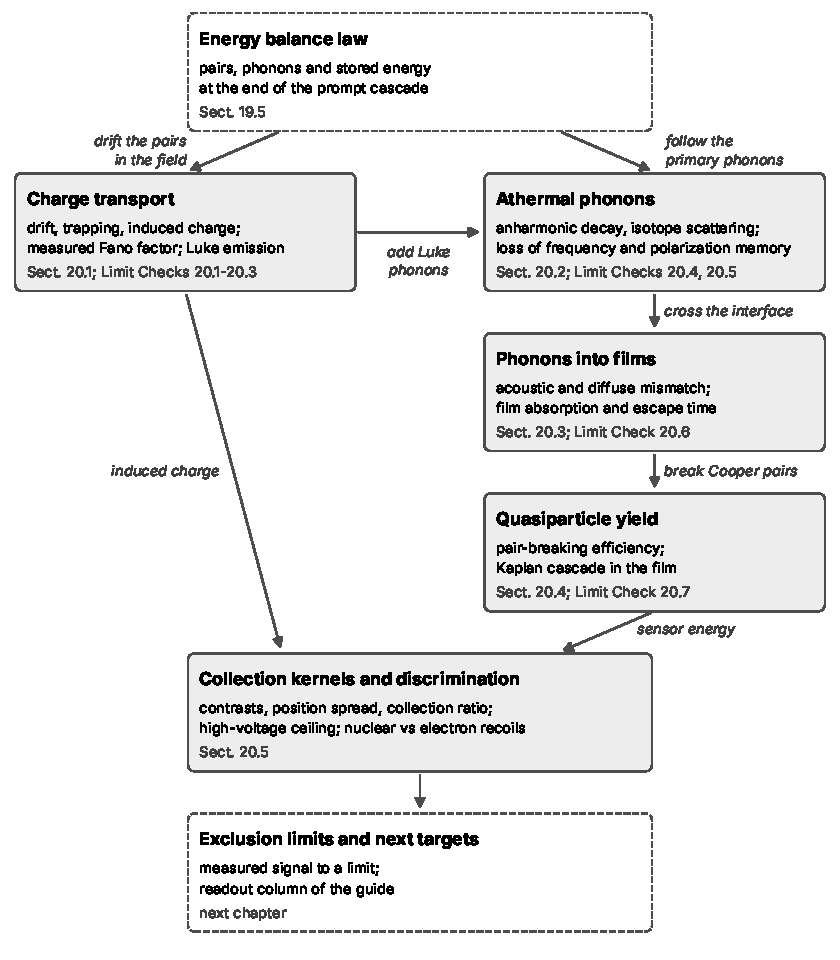
\includegraphics[width=0.85\linewidth]{figures/ch20/map20.pdf}
  \caption{Charge, phonon and quasiparticle readout, from the reservoirs of the energy balance law at the end of the prompt cascade (\cref{sec:19.5}) to the signals a detector records. Left: drift, trapping and the charge induced on the electrodes, with the measured Fano factor and the Luke phonons of the drifting carriers (\cref{sec:20.1}; \cref{lim:20.1a,lim:20.1b}). Right: the primary phonons and the Luke phonons decay and scatter in the substrate (\cref{sec:20.2}; \cref{lim:20.2a,lim:20.2b}), cross into the sensor films (\cref{sec:20.3}; \cref{lim:20.3a}) and break Cooper pairs there (\cref{sec:20.4}; \cref{lim:20.4a}). Both branches meet in the collection kernels, which decide whether phonon or charge readout separates nuclear from electron recoils (\cref{sec:20.5}).}
  \label{fig:20-map}
\end{figure}

\section{Charge transport and the measured charge}\label{sec:20.1}

The charge amplifier of a semiconductor detector integrates the current that flows into an electrode while the carriers move, and a carrier that is captured halfway across the crystal leaves half a charge in the integral and does half its share of Luke work. As a result, the charge we read is the pair number $N_{\mathrm{eh}}$ of \cref{sec:18.2} times a gain that depends on where the event happened and how far each carrier got, and the fluctuations of that gain add to the fluctuations of the cascade. At millikelvin temperatures the carriers drift in fields of a few V/cm, trapped charge does not escape thermally, and every drifting carrier radiates phonons. We will see that trapping lowers the read charge and the Luke heat by the same factor, but spreads the read charge in a way that no pair statistics removes.

\subsection{Induced charge and Ramo's theorem}\label{sec:20.1-ramo}

Consider electrodes $k$ held at potentials $V_k$ around a crystal with static dielectric constant $\varepsilon_0$ (a pure number in the Heaviside--Lorentz units of the book, \cref{sec:5.5}), and a point charge $q$ inside at $\vect{r}$. The charge on electrode $s$ is the sum of what the bias puts there and what $q$ induces, and in a linear medium the two add. The induced part follows from Green's reciprocity theorem. Compare two configurations of the same conductors. In the first, $q$ is at $\vect{r}$ and every electrode is grounded, and electrode $k$ carries the induced charge $Q_k^{\mathrm{ind}}$. In the second, there is no charge inside, electrode $s$ is held at unit potential and the others are grounded; the potential inside is then the \emph{weighting potential} $\varphi_s(\vect{r})$, the solution of $\nabla\cdot[\varepsilon_0(\vect{r})\nabla\varphi_s] = 0$ with $\varphi_s = 1$ on electrode $s$ and 0 on the others. Reciprocity states that the sum of the charges of one configuration times the corresponding potentials of the other is the same either way round. The first configuration has charges $Q_k^{\mathrm{ind}}$ on the electrodes and $q$ at $\vect{r}$; in the second the electrode potentials are $\delta_{ks}$ and the potential at $\vect{r}$ is $\varphi_s(\vect{r})$. The second configuration has charges only on the electrodes, and in the first all the electrodes are grounded. Hence $Q_s^{\mathrm{ind}} + q\varphi_s(\vect{r}) = 0$. When $q$ moves from $\vect{r}_1$ to $\vect{r}_2$, the external circuit must supply the change in induced charge, and the charge delivered to electrode $s$ is
\begin{equation}
  \Delta Q_s = -q\,\bigl[\varphi_s(\vect{r}_2) - \varphi_s(\vect{r}_1)\bigr] ,
  \label{eq:20.1-ramo}
\end{equation}
with the current $I_s = -q\,\vect{v}\cdot\nabla\varphi_s$ in its lead while the carrier moves at velocity $\vect{v}$. This is the Shockley--Ramo theorem~\cite{shockley1938currents,ramo1939currents}, \cite[Eq.~(2)]{lachish2017electron}. The weighting potential is a property of the electrode geometry alone. It is not the potential the carrier moves in. The applied bias, other carriers and trapped charges change the field and the trajectory, but by linearity they only add their own contributions to $Q_s$, and the charge induced by $q$ at a given point stays the same. \Cref{eq:20.1-ramo} is therefore exact in the presence of space charge.

For two planar electrodes at $z = 0$ and $z = d_{\mathrm{det}}$, the weighting potential of the electrode at $z = d_{\mathrm{det}}$ is $\varphi = z/d_{\mathrm{det}}$. Let the electrode at $z = d_{\mathrm{det}}$ collect electrons (the anode), so that holes drift toward the cathode at $z = 0$. Let a pair be born at depth $z$, and let its electron drift a path $s_e$ toward the anode and its hole a path $s_h$ toward the cathode. By \cref{eq:20.1-ramo} the pair delivers the charge $e\,\mathfrak{q}$ to the anode, with
\begin{equation}
  \mathfrak{q} = \frac{s_e + s_h}{d_{\mathrm{det}}} , \qquad 0 \le s_e \le d_{\mathrm{det}} - z, \quad 0 \le s_h \le z .
  \label{eq:20.1-qpair}
\end{equation}
A pair that is fully collected gives $\mathfrak{q} = 1$ wherever it was born, since its two carriers together cross the whole thickness $d_{\mathrm{det}}$. A pair born at the midplane gives $\frac12 + \frac16 = \frac23$ if its hole arrives at the cathode and its electron is captured a third of the way to the anode.

The same theorem gives the work of the bias. To hold electrode $k$ at $V_k$ while the charge it carries changes by $\Delta Q_k$, its source does the work $V_k\Delta Q_k$. Summing \cref{eq:20.1-ramo} over the electrodes gives the work done on a carrier that moves from $\vect{r}_1$ to $\vect{r}_2$, $-q\sum_kV_k[\varphi_k(\vect{r}_2) - \varphi_k(\vect{r}_1)]$. The sum $\varphi_{\mathrm{bias}}(\vect{r}) \equiv \sum_kV_k\varphi_k(\vect{r})$ is the potential the electrodes produce in the empty crystal, so that
\begin{equation}
  W_{\mathrm{bias}} = \sum_{\text{carriers}} q\,\bigl[\varphi_{\mathrm{bias}}(\vect{r}_{\mathrm{start}}) - \varphi_{\mathrm{bias}}(\vect{r}_{\mathrm{end}})\bigr] .
  \label{eq:20.1-work}
\end{equation}
The bias work is the carrier charge times the drop of $\varphi_{\mathrm{bias}}$ along the path, whatever space charge is present. Between two planes at $0$ and $V_{\mathrm{bias}}$, $\varphi_{\mathrm{bias}} = V_{\mathrm{bias}}z/d_{\mathrm{det}}$, and each pair contributes $eV_{\mathrm{bias}}\mathfrak{q}$: this is \cref{eq:19.5-Wbias}, $W_{\mathrm{bias}} = eV_{\mathrm{bias}}N_{\mathrm{ind}}$, with $N_{\mathrm{ind}} = \sum_i\mathfrak{q}_i$ the charge read on the anode in units of $e$. \Cref{app:D.45} shows that the Luke heat is $W_{\mathrm{bias}}$ minus the change $\Delta E_{\mathrm{es}}$ of the electrostatic energy. For a single trapped pair that change is negligible. Two charges \SI{10}{\micro m} apart in silicon have the Coulomb energy $\alpha/(\varepsilon_0r) = \SI{1.3e-5}{eV}$, with the liquid-helium value $\varepsilon_0 = 11.4$ (\cref{sec:7.4}), against the bias work $eV_{\mathrm{bias}}s/d_{\mathrm{det}} = \SI{4}{meV}$ done on a carrier over those \SI{10}{\micro m} in a \SI{1}{cm} crystal at \SI{4}{V}.

With more than two electrodes the read charge and the bias work weight a trajectory differently. The charge read on electrode $s$ follows $\varphi_s$ and the work follows $\varphi_{\mathrm{bias}}$, and the read charge and the bias work are proportional only where $\varphi_s \propto \varphi_{\mathrm{bias}}$, as for a pair of planar electrodes. Some detectors place interleaved electrodes on each face to tag events close to a surface. Near the interleaved electrodes the weighting potentials change over the electrode pitch, and a carrier that is trapped there adds to the read charge and to the bias work in proportions that differ from its share of the path. The reconstruction $E_R = E_\phi - E_QeV_{\mathrm{bias}}/\varepsilon_{\mathrm{eh}}$ of \cref{sec:19.5} subtracts the Luke heat through the read charge $E_Q$, and for carriers trapped near the faces it inherits the mismatch between the read charge and the bias work.

\subsection{Trapping and the Hecht relation}\label{sec:20.1-hecht}

A drifting carrier at millikelvin temperatures is lost when an ionized or neutral impurity captures it, with the cross-sections $\sigma_{\mathrm{cap},j}$ of \cref{sec:18.5}. If capture events are independent, the probability of surviving a further path $\dd s$ is $1 - \dd s/\lambda_{\mathrm{d}}$, and the probability of surviving a path $s$ is $\ee^{-s/\lambda_{\mathrm{d}}}$. The drift length is $\lambda_{\mathrm{d}} = 1/\sum_j\nd^{\mathrm{tr}}_j\sigma_{\mathrm{cap},j}$ for trap densities $\nd^{\mathrm{tr}}_j$ and cross-sections taken per unit path; with a trapping time $\tau_{\mathrm{tr}}$ instead, $\lambda_{\mathrm{d}} = v_{\mathrm{dr}}\tau_{\mathrm{tr}}$ with the drift velocity $v_{\mathrm{dr}}$. Electrons and holes have separate drift lengths, $\lambda_{\mathrm{d}}^e$ and $\lambda_{\mathrm{d}}^h$. For a path that is exponentially distributed but cut off at the distance $L$ to the electrode, the mean is $\langle\min(s, L)\rangle = \lambda_{\mathrm{d}}(1 - \ee^{-L/\lambda_{\mathrm{d}}})$.

The classic measurement of the drift length creates the charge at one face, with an alpha source or a short-range photon, so that one carrier type crosses the whole crystal and the other is collected at once. By \cref{eq:20.1-qpair} the mean collected fraction is then the mean path over $d_{\mathrm{det}}$,
\begin{equation}
  \frac{Q}{eN_{\mathrm{eh}}} = \frac{\lambda_{\mathrm{d}}}{d_{\mathrm{det}}}\bigl(1 - \ee^{-d_{\mathrm{det}}/\lambda_{\mathrm{d}}}\bigr) ,
  \label{eq:20.1-hecht}
\end{equation}
the Hecht relation~\cite{hecht1932mechanismus}, \cite[Eqs.~(1)--(4)]{lachish2017electron}. It is linear in $\lambda_{\mathrm{d}}$ for $\lambda_{\mathrm{d}} \ll d_{\mathrm{det}}$, where the carriers stop after a mean path $\lambda_{\mathrm{d}}$, and approaches $1 - d_{\mathrm{det}}/2\lambda_{\mathrm{d}}$ for $\lambda_{\mathrm{d}} \gg d_{\mathrm{det}}$. Dark-matter events happen anywhere in the bulk, and both carriers then drift. With the cut-off mean path for each carrier, a pair at depth $z$ induces on average
\begin{equation}
  \bar{\mathfrak{q}}(z) = \frac{\lambda_{\mathrm{d}}^e}{d_{\mathrm{det}}}\Bigl(1 - \ee^{-(d_{\mathrm{det}} - z)/\lambda_{\mathrm{d}}^e}\Bigr) + \frac{\lambda_{\mathrm{d}}^h}{d_{\mathrm{det}}}\Bigl(1 - \ee^{-z/\lambda_{\mathrm{d}}^h}\Bigr) ,
  \label{eq:20.1-hecht2}
\end{equation}
and averaging over a uniform depth,
\begin{equation}
  \langle\bar{\mathfrak{q}}\rangle = \sum_{c = e, h}\frac{\lambda_{\mathrm{d}}^c}{d_{\mathrm{det}}}\Bigl[1 - \frac{\lambda_{\mathrm{d}}^c}{d_{\mathrm{det}}}\bigl(1 - \ee^{-d_{\mathrm{det}}/\lambda_{\mathrm{d}}^c}\bigr)\Bigr] \simeq 1 - \frac{d_{\mathrm{det}}}{6\lambda_{\mathrm{d}}^e} - \frac{d_{\mathrm{det}}}{6\lambda_{\mathrm{d}}^h} .
  \label{eq:20.1-qavg}
\end{equation}
At second order in $d_{\mathrm{det}}/\lambda_{\mathrm{d}}$ each carrier adds $+d_{\mathrm{det}}^2/24\lambda_{\mathrm{d}}^2$, so the leading correction is accurate to a fraction $d_{\mathrm{det}}/4\lambda_{\mathrm{d}}$ of itself. Each carrier of a bulk event loses a third of what the carrier of a face event loses at the same drift length: for $\lambda_{\mathrm{d}} \gg d_{\mathrm{det}}$ the loss over a path $L$ is $L^2/2\lambda_{\mathrm{d}}d_{\mathrm{det}}$, and the mean square path to an electrode is $d_{\mathrm{det}}^2/3$. \Cref{fig:20-hecht} compares a face event, a uniform bulk event and an event at the midplane. At $\lambda_{\mathrm{d}} = d_{\mathrm{det}}$ the face event collects 0.632 of its charge, the uniform bulk event 0.736 and the midplane event 0.787; at $\lambda_{\mathrm{d}} = 10\,d_{\mathrm{det}}$ the face and bulk values are 0.952 and 0.968. The dependence of the induced charge on depth, \cref{fig:20-hecht}(b), turns trapping into a spread of the read charge (\cref{sec:20.1-fano}).

\begin{figure}[tbp]
  \centering
  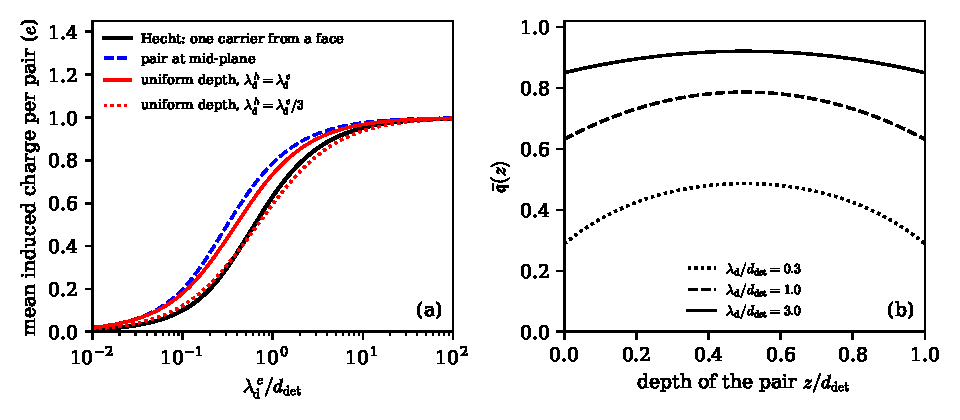
\includegraphics[width=\linewidth]{figures/ch20/fig20_1.pdf}
  \caption{Charge collection with exponential trapping in a planar detector of thickness $d_{\mathrm{det}}$. (a)~Mean induced charge per pair, in units of $e$, against the electron drift length: the Hecht relation \cref{eq:20.1-hecht} for one carrier crossing from a face (black), a pair at the midplane with equal drift lengths (blue dashed), and the depth average \cref{eq:20.1-qavg} for uniform events with $\lambda_{\mathrm{d}}^h = \lambda_{\mathrm{d}}^e$ (red) and $\lambda_{\mathrm{d}}^h = \lambda_{\mathrm{d}}^e/3$ (red dotted, an illustrative ratio). (b)~Mean induced charge of a pair against its depth, \cref{eq:20.1-hecht2} with equal drift lengths $0.3$, $1$ and $3\,d_{\mathrm{det}}$; the electron-collecting electrode is at $z = d_{\mathrm{det}}$.}
  \label{fig:20-hecht}
\end{figure}

Hecht wrote the drift length as $\lambda_{\mathrm{d}} = \mu_{\mathrm{mob}}\tau_{\mathrm{tr}}V_{\mathrm{bias}}/d_{\mathrm{det}}$, for a drift velocity proportional to the field, $v_{\mathrm{dr}} = \mu_{\mathrm{mob}}\mathcal{E}$ with mobility $\mu_{\mathrm{mob}}$, and a field-independent trapping time. The standard way to obtain the mobility--lifetime product is to measure $Q$ against the bias and fit \cref{eq:20.1-hecht} in this form. Neither the proportional drift velocity nor the field-independent trapping time enters the derivation above, which needs only exponential survival along the path. At millikelvin temperatures both assumptions fail. A carrier accelerates until it moves faster than sound and then sheds its energy into Luke phonons (\cref{sec:20.1-luke}); its speed stays within a few times the sound speed, and the largest momentum it reaches grows only as the cube root of the field~\cite[Eqs.~(24)--(25)]{leman2012invited}. If the capture cross-section per unit path does not depend on the carrier speed, $\lambda_{\mathrm{d}}$ is independent of the bias and the collected fraction does not change with the bias. If capture is a rate at fixed trapping time, $\lambda_{\mathrm{d}} = v_{\mathrm{dr}}\tau_{\mathrm{tr}}$ stops growing once the velocity saturates, and the collected fraction saturates below one.

\begin{limitbox}[Hecht collection][lim:20.1a]
For charge created at one face and drifting in a uniform field~\cite{hecht1932mechanismus}, \cite[Eqs.~(1)--(4)]{lachish2017electron}: $Q/eN_{\mathrm{eh}} = (\lambda_{\mathrm{d}}/d_{\mathrm{det}})(1 - \ee^{-d_{\mathrm{det}}/\lambda_{\mathrm{d}}})$ with $\lambda_{\mathrm{d}} = \mu_{\mathrm{mob}}\tau_{\mathrm{tr}}V_{\mathrm{bias}}/d_{\mathrm{det}}$.
\par\smallskip
{\centering
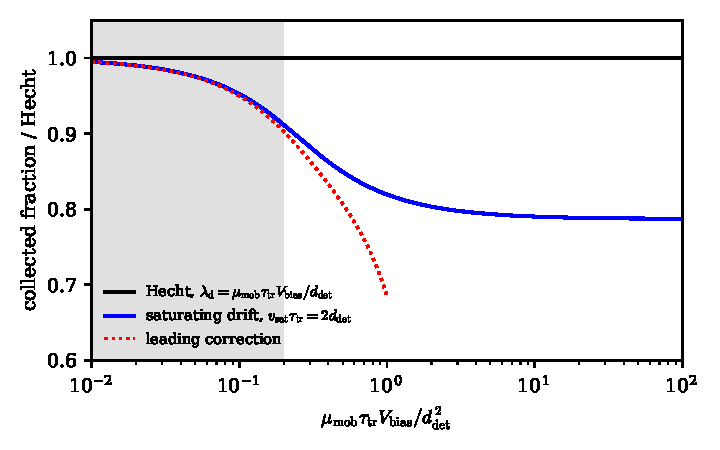
\includegraphics[width=\linewidth]{figures/ch20/limit20_1a.pdf}
\captionof{figure}{Collected fraction with a saturating drift velocity divided by the Hecht relation, against the bias in units of $d_{\mathrm{det}}^2/\mu_{\mathrm{mob}}\tau_{\mathrm{tr}}$. Blue: \cref{eq:20.1-hecht} with $\lambda_{\mathrm{d}} = v_{\mathrm{dr}}\tau_{\mathrm{tr}}$ and the interpolation $v_{\mathrm{dr}} = \mu_{\mathrm{mob}}\mathcal{E}/(1 + \mu_{\mathrm{mob}}\mathcal{E}/v_{\mathrm{sat}})$, at $v_{\mathrm{sat}}\tau_{\mathrm{tr}} = 2\,d_{\mathrm{det}}$ (an illustrative value). Red dotted: the leading correction, $\lambda_{\mathrm{d}} = \mu_{\mathrm{mob}}\tau_{\mathrm{tr}}\mathcal{E}(1 - \mu_{\mathrm{mob}}\mathcal{E}/v_{\mathrm{sat}})$. Gray: $\mu_{\mathrm{mob}}\mathcal{E} \le 0.1\,v_{\mathrm{sat}}$, where the deficit relative to the Hecht relation is at most \SI{8.9}{\percent}. At high bias the collected fraction saturates at 0.787 of the charge instead of approaching one.}\label{fig:20-limit-hecht}
\par}
\smallskip
Once the drift velocity no longer follows the field, the collected charge stops rising with the bias, and a fit of the Hecht form returns a mobility--lifetime product that depends on the bias range used.
\end{limitbox}

The deficit of the collected fraction relative to the Hecht relation is $\mu_{\mathrm{mob}}\mathcal{E}/v_{\mathrm{sat}}$ to first order, since the collection is linear in $\lambda_{\mathrm{d}}$ while $\lambda_{\mathrm{d}} \ll d_{\mathrm{det}}$. If the survival law is not exponential, as when the trap occupation changes during the drift, \cref{eq:20.1-hecht} itself changes.

\subsection{Bias work with trapping}\label{sec:20.1-work}

Trapping lowers the Luke heat with the read charge. On average over a uniform depth, \cref{eq:20.1-work} gives $W_{\mathrm{bias}} = eV_{\mathrm{bias}}N_{\mathrm{eh}}\langle\bar{\mathfrak{q}}\rangle$, and for an electron recoil that deposits $\omega$ the Luke phonon energy is $g_{\mathrm{Luke}}\langle\bar{\mathfrak{q}}\rangle\,\omega$, with the Luke gain $g_{\mathrm{Luke}} = eV_{\mathrm{bias}}/\varepsilon_{\mathrm{eh}}$ of \cref{sec:19.5}. The published phonon energy (\cref{lim:20.1b}) counts every pair as fully collected.

\begin{limitbox}[Bias work and the Luke phonon energy][lim:20.1b]
The phonon energy of $n_Q$ pairs drifted across the bias $V_{\mathrm{bias}}$ is $E_\phi = E_R + n_QeV_{\mathrm{bias}}$, with Luke part $n_QeV_{\mathrm{bias}}$~\cite[Eq.~(1)]{agnese2018nuclear}.
\par\smallskip
{\centering
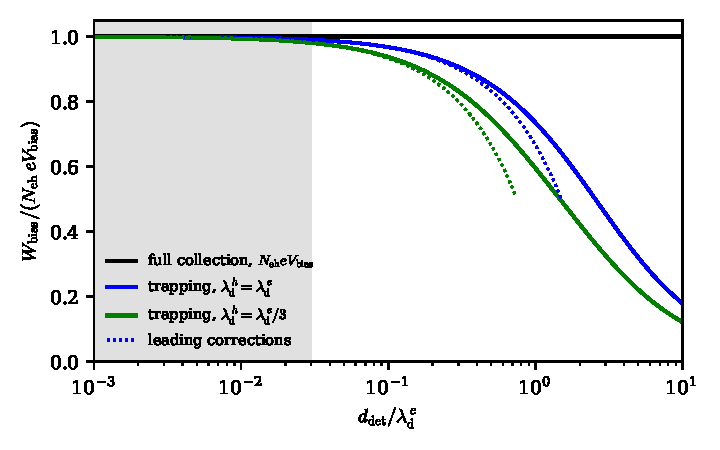
\includegraphics[width=\linewidth]{figures/ch20/limit20_1b.pdf}
\captionof{figure}{Bias work of uniformly distributed events with exponential trapping, \cref{eq:20.1-work} with the depth average \cref{eq:20.1-qavg}, over the full-collection value $N_{\mathrm{eh}}eV_{\mathrm{bias}}$, against the crystal thickness in units of the electron drift length. Blue: equal drift lengths; green: $\lambda_{\mathrm{d}}^h = \lambda_{\mathrm{d}}^e/3$ (an illustrative ratio). Dotted: the leading correction $1 - d_{\mathrm{det}}/6\lambda_{\mathrm{d}}^e - d_{\mathrm{det}}/6\lambda_{\mathrm{d}}^h$. Gray: $d_{\mathrm{det}} \le 0.030\,\lambda_{\mathrm{d}}$, where the work is within \SI{1}{\percent} of full collection for equal drift lengths ($d_{\mathrm{det}} \le 0.015\,\lambda_{\mathrm{d}}^e$ for the unequal pair).}\label{fig:20-limit-work}
\par}
\smallskip
When the drift length is no longer much longer than the crystal, the Luke heat falls below $N_{\mathrm{eh}}eV_{\mathrm{bias}}$ and depends on the depth of the event; it follows the read charge, not the pair number.
\end{limitbox}

Since the read charge of a planar detector carries the same factor $\bar{\mathfrak{q}}$ as the Luke heat, event by event, the subtraction $E_QeV_{\mathrm{bias}}/\varepsilon_{\mathrm{eh}}$ removes the Luke heat of partly collected pairs exactly. Trapping also changes the signal beyond the Luke heat. A trapped carrier keeps its share of the gap energy, which the balance law counts as missing energy (\cref{sec:19.5}), and a nuclear recoil has an ionized fraction $f_{\mathrm{ion}}$ below its ionization yield if its dense track traps more often.

\subsection{Fano factor of the measured charge}\label{sec:20.1-fano}

If each pair is either collected in full or lost, independently and with the same probability $f_{\mathrm{det}}$ everywhere, the read charge is the pair number thinned binomially, and its Fano factor is $f_{\mathrm{det}}F_{\mathrm{eh}} + 1 - f_{\mathrm{det}}$ by \cref{eq:C.11-thinfano}. Trapping does not thin the pair number binomially. A trapped carrier leaves a partial charge, and the mean collection depends on the depth of the event. Let the event be at $\vect{r}$, and let the induced charges $\mathfrak{q}_i$ of its pairs, \cref{eq:20.1-qpair}, be independent and identically distributed given $\vect{r}$, with mean $\bar{\mathfrak{q}}(\vect{r})$ and variance $\sigma_{\mathfrak{q}}^2(\vect{r})$, and independent of the pair number. These assumptions hold when the carriers drift independently after the prompt cascade; independent drift excludes recombination and screening inside a dense track. The read charge is $N_{\mathrm{ind}} = \sum_{i=1}^{N_{\mathrm{eh}}}\mathfrak{q}_i$. At fixed $\vect{r}$, a sum of a random number of independent terms has mean $\bar N_{\mathrm{eh}}\bar{\mathfrak{q}}$ and variance $\bar N_{\mathrm{eh}}\sigma_{\mathfrak{q}}^2 + \bar{\mathfrak{q}}^2\operatorname{Var}N_{\mathrm{eh}}$, with $\operatorname{Var}N_{\mathrm{eh}} = F_{\mathrm{eh}}\bar N_{\mathrm{eh}}$. Averaging over the position with the law of total variance gives $\operatorname{Var}N_{\mathrm{ind}} = \langle\operatorname{Var}(N_{\mathrm{ind}}|\vect{r})\rangle + \operatorname{Var}_{\vect{r}}(\bar N_{\mathrm{eh}}\bar{\mathfrak{q}})$, and dividing by the mean $\bar N_{\mathrm{eh}}\langle\bar{\mathfrak{q}}\rangle$ gives
\begin{equation}
  F_{\mathrm{meas}} = \underbrace{\frac{F_{\mathrm{eh}}\langle\bar{\mathfrak{q}}^2\rangle}{\langle\bar{\mathfrak{q}}\rangle}}_{\text{cascade}} + \underbrace{\frac{\langle\sigma_{\mathfrak{q}}^2\rangle}{\langle\bar{\mathfrak{q}}\rangle}}_{\text{partial charge}} + \underbrace{\bar N_{\mathrm{eh}}\,\frac{\operatorname{Var}_{\vect{r}}\bar{\mathfrak{q}}}{\langle\bar{\mathfrak{q}}\rangle}}_{\text{position}} ,
  \label{eq:20.1-Fpos}
\end{equation}
where $\langle\cdot\rangle$ and $\operatorname{Var}_{\vect{r}}$ are taken over the distribution of event positions.

For all-or-nothing collection with one probability, $\bar{\mathfrak{q}} = f_{\mathrm{det}}$, $\sigma_{\mathfrak{q}}^2 = f_{\mathrm{det}}(1 - f_{\mathrm{det}})$ and the position term vanishes; \cref{eq:20.1-Fpos} then returns the binomial result. The unsplit excitons of \cref{eq:18.5-Fmeas} are the same thinning with $f_{\mathrm{det}} = 1 - p_{\mathrm{ns}}$, and the values of $f_{\mathrm{det}}$ of losses that act independently on each pair multiply. The partial-charge term is never larger than in the binomial case. Since $0 \le \mathfrak{q} \le 1$, $\mathfrak{q}^2 \le \mathfrak{q}$, so $\langle\mathfrak{q}^2\rangle \le \bar{\mathfrak{q}}$ and $\sigma_{\mathfrak{q}}^2 \le \bar{\mathfrak{q}}(1 - \bar{\mathfrak{q}})$ at every position. At a fixed position, a loss shared as partial charges by many pairs fluctuates less than the same mean loss concentrated on a few pairs that are lost entirely. The position term grows with $\bar N_{\mathrm{eh}}$, and its contribution to the relative variance of the read charge, $\operatorname{Var}_{\vect{r}}\bar{\mathfrak{q}}/\langle\bar{\mathfrak{q}}\rangle^2$, does not fall with energy. The position term is a spread of the gain across the crystal, which no pair statistics removes, and it dominates at large deposits.

\begin{workedexample}{The measured Fano factor at 95 percent collection in silicon}\label{we:20-fano}
Take the cascade value $F_{\mathrm{eh}} = 0.114$ of \cref{sec:18.2} and a mean collected fraction of 0.95, and compare three ways of losing the missing \SI{5}{\percent}. (\Cref{sec:20.5} uses the measured value 0.119 for electron-recoil signals.)

\emph{All-or-nothing loss, uniform.} Binomial thinning gives $0.95 \times 0.114 + 0.05 = 0.158$.

\emph{Trapping, every pair at the midplane.} With equal drift lengths, \cref{eq:20.1-hecht2} at $z = d_{\mathrm{det}}/2$ is $2(\lambda_{\mathrm{d}}/d_{\mathrm{det}})(1 - \ee^{-d_{\mathrm{det}}/2\lambda_{\mathrm{d}}})$, which equals 0.95 at $\lambda_{\mathrm{d}} = 4.83\,d_{\mathrm{det}}$. Each carrier's path is exponential with mean $\lambda_{\mathrm{d}}$, cut at $d_{\mathrm{det}}/2$, and its second moment is $\langle\min(s, L)^2\rangle = 2\lambda_{\mathrm{d}}^2[1 - \ee^{-L/\lambda_{\mathrm{d}}}(1 + L/\lambda_{\mathrm{d}})]$. The two carriers give $\sigma_{\mathfrak{q}}^2 = 0.0156$, a third of the binomial $0.95 \times 0.05 = 0.0475$. \Cref{eq:20.1-Fpos} gives $F_{\mathrm{meas}} = (0.114 \times 0.9025 + 0.0156)/0.95 = 0.125$.

\emph{Trapping, uniform depth.} Now \cref{eq:20.1-qavg} equals 0.95 at $\lambda_{\mathrm{d}} = 6.41\,d_{\mathrm{det}}$. Integrating \cref{eq:20.1-hecht2} and the variance over depth gives $\langle\bar{\mathfrak{q}}^2\rangle = 0.9026$, $\langle\sigma_{\mathfrak{q}}^2\rangle = 0.0230$ and $\operatorname{Var}_z\bar{\mathfrak{q}} = 1.16\times10^{-4}$. The cascade and partial-charge terms give 0.1325. The position term is $1.22\times10^{-4}\,\bar N_{\mathrm{eh}}$: 0.003 for a \SI{100}{eV} recoil ($\bar N_{\mathrm{eh}} = 26.7$), 0.033 at \SI{1}{keV} and 0.19 at \SI{5.9}{keV}. It equals 0.01 at 82 pairs, about \SI{0.3}{keV}.

The same mean collection thus yields a measured Fano factor between 0.125 and 0.158 at \SI{100}{eV}, depending on how the charge is lost, and nearly three times the cascade value at \SI{5.9}{keV} if the loss depends on depth. A Fano factor measured at \SI{5.9}{keV} constrains $F_{\mathrm{eh}}$ to 0.01 only if $\operatorname{Var}_z\bar{\mathfrak{q}}$ is below $6\times10^{-6}$.
\end{workedexample}

\subsection{Space charge of trapped carriers}\label{sec:20.1-space}

At millikelvin temperatures a trapped carrier is not re-emitted thermally. A donor level \SI{45}{meV} below the conduction band carries the Boltzmann factor $\ee^{-1.04\times10^4}$ at \SI{50}{mK}. A field lowers the Coulomb barrier of a charged center: the potential energy $-\alpha/(\varepsilon_0r) - e\mathcal{E}r$ of the carrier along the field has its maximum at the field separation radius $r_{\mathcal{E}} = (\alpha/\varepsilon_0e\mathcal{E})^{1/2}$ of \cref{eq:18.5-rfield}, and the field thus lowers the barrier by the Poole--Frenkel amount $2e\mathcal{E}r_{\mathcal{E}}$. In silicon that is \SI{0.45}{meV} at \SI{4}{V/cm} and \SI{2.25}{meV} at \SI{100}{V/cm}, far below \SI{45}{meV}. Thermal and field-assisted emission are frozen, and trapped charge is released only by the phonons of later events, by drifting carriers that ionize the center on impact, or by infrared light. Detectors are therefore illuminated at intervals with infrared diodes, a practice called flashing~\cite[Sect.~2]{agnese2018nuclear}; the infrared light neutralizes the ionized trapping sites and keeps trapping low. Between flashes the trapped charge accumulates and changes the field.

In a planar detector at fixed bias the field change follows from Gauss's law and the constraint that the voltage across the crystal does not change. Let $\varrho_{\mathrm{tr}}(z)$ be the net trapped charge per unit volume, averaged over the transverse directions. The field change obeys $\dd\Delta\mathcal{E}/\dd z = \varrho_{\mathrm{tr}}/\varepsilon_0$, so $\Delta\mathcal{E}(z) = \Delta\mathcal{E}(0) + \varepsilon_0^{-1}\int_0^z\varrho_{\mathrm{tr}}\,\dd z'$, and fixed bias requires $\int_0^{d_{\mathrm{det}}}\Delta\mathcal{E}\,\dd z = 0$. Solving for $\Delta\mathcal{E}(0)$ and integrating by parts gives
\begin{equation}
  \Delta\mathcal{E}(z) = \frac{1}{\varepsilon_0}\left[\int_0^z\varrho_{\mathrm{tr}}(z')\,\dd z' - \frac{1}{d_{\mathrm{det}}}\int_0^{d_{\mathrm{det}}}(d_{\mathrm{det}} - z')\,\varrho_{\mathrm{tr}}(z')\,\dd z'\right] ,
  \label{eq:20.1-dE}
\end{equation}
in Heaviside--Lorentz units, with $\varepsilon_0$ the static dielectric constant; in SI units multiply $\varepsilon_0$ by the vacuum permittivity $\varepsilon_0^{\mathrm{SI}}$. A sheet of $\nd_{\mathrm{sh}}$ charges $e$ per unit area at depth $z_0$ makes the field jump by $e\nd_{\mathrm{sh}}/\varepsilon_0$ across it, with the change $-e\nd_{\mathrm{sh}}(d_{\mathrm{det}} - z_0)/\varepsilon_0d_{\mathrm{det}}$ below and $+e\nd_{\mathrm{sh}}z_0/\varepsilon_0d_{\mathrm{det}}$ above, so the largest change lies between one half and the whole jump. For any distribution of one sign with $\nd_{\mathrm{sh}}$ charges per unit area in all, both terms in the bracket of \cref{eq:20.1-dE} lie between 0 and $e\nd_{\mathrm{sh}}$, so their difference does not exceed $e\nd_{\mathrm{sh}}$. Hence the sheet bound
\begin{equation}
  \max_z|\Delta\mathcal{E}(z)| \le \frac{e\nd_{\mathrm{sh}}}{\varepsilon_0} ,
  \label{eq:20.1-sheet}
\end{equation}
which a sheet approaches as it nears a face. There, however, the whole change lies in the thin slab between the sheet and the nearer electrode, and the field in the rest of the crystal is unchanged: the charge only images onto that electrode. A sheet at depth $z_0$ changes the field on its far side by $e\nd_{\mathrm{sh}}z_0/\varepsilon_0d_{\mathrm{det}}$, so a distortion over a finite part of the drift region needs more charge than the sheet bound \cref{eq:20.1-sheet} implies, and a sheet at the midplane, which changes the field by half the jump over the whole crystal, needs twice the charge of the sheet bound. Charges of both signs give at most $e(\nd_{\mathrm{sh}}^+ + \nd_{\mathrm{sh}}^-)/\varepsilon_0$, and less where electrons and holes trapped at similar depths cancel.

We measure the distortion by $\xi_{\mathrm{SC}} \equiv \max_z|\Delta\mathcal{E}|/\mathcal{E}$. In silicon, with $\varepsilon_0 = 11.4$, one charge per square centimeter moves the field by \SI{1.59e-7}{V/cm}. A distortion $\xi_{\mathrm{SC}} = \SI{1}{\percent}$ at \SI{1}{V/cm} then needs at least \SI{6.3e4}{cm^{-2}}. A sheet next to a face reaches this sheet bound but distorts only a vanishing slab; a sheet at the midplane distorts the whole crystal by \SI{1}{\percent} at \SI{12.6e4}{cm^{-2}}. At the \SI{4}{V/cm} of the calibration of \cref{sec:19.5} both sheets need four times more charge. Between flashes the trapped density grows as $\nd_{\mathrm{sh}}(t) \approx R\bar N_{\mathrm{eh}}p_{\mathrm{tr}}t$, for $R$ events per unit area and time with $\bar N_{\mathrm{eh}}$ pairs each, of which a fraction $p_{\mathrm{tr}}$ leaves a trapped charge of the dominant sign. A trapping probability of \SI{12.7}{\percent} is the value used to model a silicon detector that resolves single charges~\cite{albakry2023first}. With it as $p_{\mathrm{tr}}$, \SI{100}{eV} events at \SI{1}{Hz} on \SI{1}{cm^2} reach a distortion of \SI{1}{\percent} at \SI{1}{V/cm} over the whole crystal in 10 hours (the near-face limit in 5), and a calibration at a thousand times that rate within a minute.

\Cref{eq:20.1-ramo,eq:20.1-work} stay exact; the distortion acts through the trajectories. It changes the drift velocity along the path and, where capture depends on the carrier speed, the drift length; in three dimensions it bends the field lines, and carriers near the sides of the crystal can end on bare surfaces instead of electrodes. The energy stored in the field of the trapped charge is part of the electrostatic term $\Delta E_{\mathrm{es}}$ that separates the Luke heat from the bias work (\cref{app:D.45}). The trapped populations, the field and the rate of delayed charge released by later events therefore all depend on the exposure since the last flash.

\subsection{Luke-phonon emission}\label{sec:20.1-luke}

A carrier that moves faster than the longitudinal sound speed $c_{\mathrm{LA}}$ can emit a longitudinal acoustic phonon and conserve both energy and momentum; a slower one cannot. This emission above the sound speed is the acoustic analogue of Cherenkov radiation, and the phonons emitted are the Luke phonons that carry the bias work. The emission rate follows from the golden rule with the deformation-potential vertex of \cref{eq:6.2-D}. Take a carrier of isotropic mass $m$, energy $k^2/2m$ and momentum $\vect{k}$, and an isotropic deformation potential $D^n$, which couples it to longitudinal phonons only. A phonon of wavevector $\vect{Q}$ then has the matrix element $|M_Q|^2 = (D^n)^2Q/(2\rho_T\Vol c_{\mathrm{LA}})$ in a crystal of volume $\Vol$ and mass density $\rho_T$, the vertex of \cref{sec:6.2} with the volume normalization. Luke phonons carry about a meV, more than ten kelvin. At detector temperatures absorption and stimulated emission are therefore negligible, and
\begin{equation*}
  \varGamma_{\mathrm{L}}(k) = 2\pi\sum_{\vect{Q}}|M_Q|^2\,\delta\Bigl(\frac{k^2}{2m} - \frac{(\vect{k} - \vect{Q})^2}{2m} - c_{\mathrm{LA}}Q\Bigr) .
\end{equation*}
With $\theta$ the angle between $\vect{Q}$ and $\vect{k}$, the argument of the delta function vanishes at $Q_* = 2(k\cos\theta - k_{\mathrm{s}})$, where $k_{\mathrm{s}} = mc_{\mathrm{LA}}$ is the momentum of a carrier moving at the sound speed, and the derivative of the argument with respect to $Q$ there has magnitude $Q_*/2m$. A positive root requires $\cos\theta > k_{\mathrm{s}}/k$, and so $k > k_{\mathrm{s}}$: the Cherenkov condition. With $\sum_{\vect{Q}} = V\int\dd^3Q/(2\pi)^3$, the azimuthal integral gives $2\pi$, so the prefactor is $2\pi\cdot2\pi/(2\pi)^3 = 1/2\pi$, and the radial integral $\int Q^2\dd Q\,Q\,\delta(\ldots)$ gives $Q_*^3\cdot2m/Q_*$. Hence
\begin{equation*}
  \varGamma_{\mathrm{L}}(k) = \frac{(D^n)^2m}{2\pi\rho_Tc_{\mathrm{LA}}}\int_{k_{\mathrm{s}}/k}^1 Q_*^2\,\dd\cos\theta = \frac{(D^n)^2m}{2\pi\rho_Tc_{\mathrm{LA}}}\,\frac{4k^2}{3}\Bigl(1 - \frac{k_{\mathrm{s}}}{k}\Bigr)^3 .
\end{equation*}
With the scattering length $l_0 = \pi\rho_T/(2m^3(D^n)^2)$, a length that collects the coupling and the carrier mass, the rate is
\begin{equation}
  \varGamma_{\mathrm{L}}(k) = \frac{c_{\mathrm{LA}}}{3l_0}\Bigl(\frac{k}{k_{\mathrm{s}}}\Bigr)^2\Bigl(1 - \frac{k_{\mathrm{s}}}{k}\Bigr)^3 \qquad (k > k_{\mathrm{s}}),
  \label{eq:20.1-luke}
\end{equation}
and the phonon is emitted at the polar angle $\theta$ with the probability density $\propto(\cos\theta - k_{\mathrm{s}}/k)^2\sin\theta$, up to $\cos\theta = k_{\mathrm{s}}/k$. Leman~\cite[Eq.~(22)]{leman2012invited} and the authors of the G4CMP (Geant4 Condensed Matter Physics) toolkit~\cite[Eq.~(9)]{kelsey2023g4cmp} print an angular law that integrates to \cref{eq:20.1-luke}, but the total rates printed beside that angular law~\cite[Eq.~(21)]{leman2012invited}, \cite[Eq.~(8)]{kelsey2023g4cmp} are lower by the factor $k_{\mathrm{s}}/k$.

The phonon energy is $c_{\mathrm{LA}}Q_* = 2c_{\mathrm{LA}}k(\cos\theta - k_{\mathrm{s}}/k)$. The average over the angular distribution, in which $u = \cos\theta - k_{\mathrm{s}}/k$ is weighted by $u^2$ on $[0, 1 - k_{\mathrm{s}}/k]$ and so has the mean $\frac34(1 - k_{\mathrm{s}}/k)$, gives
\begin{equation}
  \langle E_{\mathrm{L}}\rangle = \frac32\,mc_{\mathrm{LA}}^2\Bigl(\frac{k}{k_{\mathrm{s}}} - 1\Bigr), \qquad E_{\mathrm{L}}^{\max} = 2mc_{\mathrm{LA}}^2\Bigl(\frac{k}{k_{\mathrm{s}}} - 1\Bigr) .
  \label{eq:20.1-Eluke}
\end{equation}
The energy scale is set by the carrier mass and the sound speed. For silicon holes, with the isotropic mass $0.5\,m_e$, $D^n = \SI{5.0}{eV}$ and $c_{\mathrm{LA}} = \SI{9.0}{km/s}$ of the CDMS transport model~\cite[Table~II]{leman2012invited}, $mc_{\mathrm{LA}}^2 = \SI{0.230}{meV}$, $l_0 = \SI{7.5}{\micro m}$ and $c_{\mathrm{LA}}/3l_0 = \SI{4.0e8}{s^{-1}}$. A hole at twice the sound speed emits phonons at \SI{2.0e8}{s^{-1}}, with a mean energy of \SI{0.35}{meV} and at most \SI{0.46}{meV}.

A transport Monte Carlo of silicon electrons gives a mean Luke phonon energy of \SI{0.84}{meV} at \SI{1}{V/cm} (\cref{sec:20.5-meanfield}). Luke phonons are born at one to a few meV, between the pair-breaking energy $2\Delta_{\mathrm{BCS}} = \SI{0.36}{meV}$ of bulk aluminum (\cref{sec:1.5}) and the optical-phonon energies near \SI{60}{meV} at which the primary phonons start. Since the emitted energy is weighted by $u^3$, the fraction of it below an energy $E_{\mathrm{c}}$ is $(E_{\mathrm{c}}/E_{\mathrm{L}}^{\max})^4$ for a carrier at one speed. Transport decides whether the sensor films then absorb the Luke phonons as efficiently as the down-converted primaries, and so decides the sign of $\mathfrak{r}_{\mathrm{coll}} - 1$ in the calibration of \cref{sec:19.5} (\cref{sec:20.5}).

\subsection{Open problems}\label{sec:20.1-open}

The emission rates of trapped charge at millikelvin temperatures are not known, and so neither the release of trapped charge over a run nor the growth of the space-charge field between flashes is known. The emission rate of each trap class is the sum of the phonon flux times a phonon-ionization cross-section, the flux of drifting carriers times an impact-ionization cross-section, and a term from the infrared illumination. A neutral shallow donor needs a phonon above its binding energy, \SI{45}{meV} or \SI{10.9}{THz} for phosphorus in silicon, and phonons above \SI{45}{meV} decay within about a nanosecond (\cref{sec:20.2}), so they ionize only near the track of a later event. Luke phonons cannot ionize neutral centers but can ionize the over-charged states $\mathrm{D}^-$ and $\mathrm{A}^+$, which bind their extra carrier by a few meV and which flashing itself populates. No calculation gives the phonon-ionization or the impact-ionization cross-section of these centers at the carrier and phonon energies that matter. Without these cross-sections the trapped populations, the field distortion $\xi_{\mathrm{SC}}$ and the delayed charge cannot be followed through an exposure history.

The spectrum that the Luke rate \cref{eq:20.1-luke} produces is tested only indirectly. The rate keeps longitudinal phonons only, whereas the uniaxial deformation potential $\Xi_u$ couples the electrons of the silicon valleys to transverse phonons with the vertex $\Xi_u\sin\theta\cos\theta$ (\cref{sec:6.2}), and holes couple to them as well; transverse emission starts at the lower transverse sound speed and gives softer phonons. The Luke rate also assumes one isotropic deformation potential and a parabolic band, and treats the anisotropic electron valleys by a Herring--Vogt transformation that does not conserve the phonon momentum exactly. Transport models reproduce the measured drift velocity against field in germanium. The drift velocity tests the rate of momentum loss along the field, an angular moment of the emission, and not the energy spectrum of the Luke phonons, on which their collection depends. A rate with both acoustic branches and the valley-resolved deformation potentials, checked against a phonon signal measured at fixed field, would settle the question of the Luke spectrum.

A transport simulation of a detector must pass the tests of this section before its collection kernels are used. The tests are the Hecht relation at a known trap density, the charge sum (charge read on all electrodes plus the trapped charges weighted by their weighting potentials equals the charge created), the bias work \cref{eq:20.1-work} and the measured Fano factor \cref{eq:20.1-Fpos}. No validation of a transport engine against these tests has been published at the level of a few percent that the collection ratio of \cref{sec:19.5} requires.

\section{Athermal phonons in the substrate}\label{sec:20.2}

At the partition time of \cref{sec:19.1}, some \SI{100}{ps} after a \SI{100}{eV} electron recoil in silicon, about \SI{69}{eV} sits in phonons of tens of meV, some two thousand of them near the point of the event. A sensor film on the surface absorbs phonons microseconds later, after they have decayed several times and scattered off isotopes hundreds of times. The phonons of a nuclear recoil of the same energy start from a different spectrum. If that difference survived to the sensor, a phonon readout could tell the two recoils apart by what it absorbs, and the phonon collection of a nuclear recoil could differ from that of the electron recoil used to calibrate it (\cref{sec:19.5}). Two rates decide the question: anharmonic decay, which scales as the fifth power of the phonon energy, and isotope scattering, which scales as the fourth. Together they drive every hard spectrum toward one shape that depends on time only through a single energy scale, and they leave the energy born at low phonon energies as the difference that a linear readout can still see.

\subsection{Prompt phonons at the partition time}\label{sec:20.2-prompt}

The phonons that carry the prompt energy $E_{\mathrm{prompt}} = E_{\mathrm{phon}}(t_{\mathrm{pr}})$ of \cref{sec:19.5-law} are \emph{athermal}. Their energies $E_{\mathrm{ath}}$, from meV to tens of meV, exceed the thermal energy of \SI{0.86}{\micro eV} at \SI{10}{mK} by four orders of magnitude or more, and their population is far from equilibrium. It is also dilute: about 2300 phonons of \SI{30}{meV}, even if confined to a sphere of radius \SI{1}{\micro m}, share $6\times10^{11}$ modes, an occupation of $4\times10^{-9}$. They do not interact with each other. Each phonon interacts with the static crystal alone, scattering off the random isotope masses, and decays spontaneously through the cubic anharmonicity; at \SI{10}{mK} the Bose factors of \cref{eq:5.7-gamma} vanish, leaving spontaneous decay. The transport is linear in the deposit, and the birth spectrum is the initial condition of a linear evolution.

The two recoils make their phonons in different ways. In an electron recoil the hot carriers of \cref{chap:18} lose most of their energy by emitting optical and intervalley phonons (\cref{sec:18.1-ph}). An optical phonon lives \SI{3.7}{ps} (\cref{we:5-klemens}) and decays mostly into a longitudinal acoustic phonon near \SI{42}{meV} and a transverse one near \SI{22}{meV} (\cref{sec:5.7}). By $t_{\mathrm{pr}}$ the optical phonons are gone, and the population is acoustic and hard. Below the optical energy a carrier can emit only acoustic phonons, and momentum conservation caps their energy at $2c_{\mathrm{LA}}k$ for a carrier of momentum $k$. For a silicon electron with the density-of-states mass $0.32\,m_e$ of one valley, the cap is \SI{8.7}{meV} at a kinetic energy of \SI{64}{meV} and \SI{6.0}{meV} at \SI{30}{meV}. Suppose each carrier enters this regime with a kinetic energy spread uniformly below $\omega_{\mathrm{opt}}$. Each of the two carriers then has the mean kinetic energy $\omega_{\mathrm{opt}}/2$, so each pair sheds on average $\omega_{\mathrm{opt}}$ in phonons below about 6 to \SI{9}{meV}, and the soft fraction of the deposit is
\begin{equation}
  f_{\mathrm{s}} \simeq \frac{\omega_{\mathrm{opt}}}{\varepsilon_{\mathrm{eh}}} .
  \label{eq:20.2-fs}
\end{equation}
This estimate gives \SI{1.7}{\percent} in silicon, with the measured $\omega_{\mathrm{opt}} = \SI{64.1}{meV}$ (\cref{sec:5.2}) and $\varepsilon_{\mathrm{eh}} = \SI{3.75}{eV}$ (\cref{sec:18.2}), and \SI{1.3}{\percent} in germanium, with \SI{37.6}{meV} (\cref{tab:5-phonons}) and \SI{2.96}{eV}~\cite[Table~I]{leman2012invited}. The gap energy $N_{\mathrm{eh}}\Eg$, \SI{31}{\percent} of an electron recoil in silicon, is not part of the prompt population. It returns as phonons later, where and with which spectrum the release channel decides (\cref{sec:19.5,sec:20.5}).

In a nuclear recoil below the displacement threshold the whole deposit is heat (\cref{sec:19.1}). For small recoils the phonons that the nuclear response creates are the final state, with the energy-weighted phonon content of \cref{sec:11.3}. Above a few eV the created spectrum comes from the molecular dynamics of \cref{app:E.23}, which has not been tabulated. A recoil that thermalizes locally fills the modes in proportion to their density of states, and its spectrum is hard as well. Both populations are hard, between about 4 and \SI{15}{THz} in silicon, and they differ in branch content and in shape; only the electron recoil carries the soft fraction $f_{\mathrm{s}}$.

\subsection{Anharmonic down-conversion}\label{sec:20.2-anh}

The linewidth \cref{eq:5.7-gamma} at $T = 0$ gives the decay rate of any phonon. For an acoustic phonon of long wavelength it takes a simple form, because both of its ingredients, the vertex and the phase space, scale as powers of the frequency. Translation invariance makes the vertex small. By the sum rule \cref{eq:5.7-asr}, the third-order constants vanish when summed over the positions of any one atom. In \cref{eq:5.7-V3} the term of zeroth order in each wavevector cancels whenever the polarizations are those of a uniform translation, as they are for acoustic phonons at small $Q$. The first surviving term carries one power of each wavevector, $Q_1Q_2Q_3$, multiplied by the third-order elastic constants. With the prefactor $(\omega_1\omega_2\omega_3)^{-1/2}$ and the linear dispersion $\omega_i = c_iQ_i$, the vertex becomes
\begin{equation}
  V^{(3)}(1,2,3) = (\omega_1\omega_2\omega_3)^{1/2}\,v_3(\hat{\vect{Q}}_i, \nu_i) ,
  \label{eq:20.2-V3}
\end{equation}
with $v_3$ a function of the directions and branches alone. The squared vertex of a decay $\omega \to \omega_1 + \omega_2$ is then $\omega^3y(1 - y)|v_3|^2$, with $y = \omega_1/\omega$. The phase space is the sum over $\vect{Q}_1$ at fixed $\vect{Q}_2 = \vect{Q} - \vect{Q}_1$. In polar coordinates about $\vect{Q}$, the angle integral of the energy delta function is $\int\dd\cos\theta\,\delta(\omega - c_1Q_1 - c_2Q_2) = Q_2/(c_2QQ_1)$, since $\dd Q_2/\dd\cos\theta = -QQ_1/Q_2$. The remaining integral $(2\pi/c_2Q)\int\dd Q_1\,Q_1Q_2$ scales as $\omega^2$. The angles at which the decay happens are fixed by $y$ and the speeds, so $v_3$ contributes a function of $y$ only, and the rate scales as $\omega^3\times\omega^2$:
\begin{equation}
  \varGamma_{\mathrm{anh}} = A_{\mathrm{anh}}\Bigl(\frac{E_{\mathrm{ath}}}{h}\Bigr)^5 .
  \label{eq:20.2-anh}
\end{equation}
This is \cref{eq:E.12-anh}. The constant $A_{\mathrm{anh}}$ depends on the second- and third-order elastic constants and on the branch of the decaying phonon. The derivation needs normal processes ($\vect{G} = 0$) and frequencies low enough for linear dispersion, the same long-wavelength condition as for the Rayleigh law of isotope scattering below.

Not every branch decays. In the isotropic continuum a transverse phonon cannot decay at all. Its energy $c_{\mathrm{T}}Q$ would have to equal $c_1Q_1 + c_2Q_2$, with both speeds at least $c_{\mathrm{T}}$, the lowest speed, and with $Q_1 + Q_2 \ge Q$ by the triangle inequality. The only solutions are collinear decays into two transverse phonons, for which the isotropic vertex vanishes. A longitudinal phonon decays through the channels $\mathrm{L}\to\mathrm{L}'+\mathrm{T}'$ and $\mathrm{L}\to\mathrm{T}+\mathrm{T}$, with the daughter energies distributed as in \cref{app:E.12}. Anisotropy and dispersion open slow decays of transverse phonons in real crystals, which transport codes neglect~\cite[Sect.~2.2.2]{kelsey2023g4cmp}. In the isotropic continuum $A_{\mathrm{anh}}$ is a closed form in five elastic constants, the two Lamé constants and three third-order combinations~\cite[Eqs.~(1), (2)]{hernandez2025modeling}. For silicon, Tamura's calculation gives $A_{\mathrm{anh}} = \SI{7.41e-56}{s^4}$~\cite[Table~I]{leman2012invited}, and a recalculation from cryogenic elastic constants gives \SI{1.15e-55}{s^4}~\cite[Table~3]{hernandez2025modeling}. For germanium the published values spread over a factor of ten, from \SI{1.61e-55}{s^4}~\cite{hertel2012phonon} through \SI{6.8e-55}{s^4} in the recalculation to \SI{1.65e-54}{s^4}. Two of them are both attributed to Tamura's work yet disagree by a factor 2.6: \SI{6.43e-55}{s^4}~\cite[Table~I]{leman2012invited} and \SI{1.65e-54}{s^4}~\cite[Table~3]{hernandez2025modeling}. No direct measurement exists for either crystal, and we use the slowest germanium value, \SI{1.61e-55}{s^4}. A longitudinal phonon at the top of the silicon acoustic band, \SI{15}{THz}, decays in \SI{18}{ps}; one at \SI{1}{THz} lives \SI{14}{\micro s}.

The constants come from the elastic tensors. The second-order constants are measured or computed as in \cref{app:E.4}; the third-order ones follow from the same finite-strain calculations taken one order further, or from ultrasonic measurements under stress. \Cref{app:E.12} sets out how the two rates enter a transport Monte Carlo of a whole detector, together with the kinematics of the daughters and the focusing of the group velocities. \Cref{app:E.25} specifies how the created-phonon spectra of the two recoils are carried through it to the sensors.

\subsection{Isotope scattering}\label{sec:20.2-iso}

Natural silicon is \SI{92.2}{\percent} $^{28}$Si, \SI{4.7}{\percent} $^{29}$Si and \SI{3.1}{\percent} $^{30}$Si, and a phonon sees the random masses as point scatterers. Write the isotope on site $I$ as a mass defect $\delta^M_I = (\bar M - M_I)/\bar M$ about the mean mass $\bar M$, whose variance over the isotopes is the mass variance $g_{\mathrm{md}} = \sum_ix_i(\delta^M_i)^2$ of \cref{app:E.12}. To lowest order in $g_{\mathrm{md}}$, the self-energy of the mass disorder in \cref{sec:11.6} gives every phonon of frequency $\omega$ the same width,
\begin{equation}
  \varGamma_{\mathrm{iso}}(\omega) = \frac{\pi}{6}\,g_{\mathrm{md}}\,\omega^2\,g_{\mathrm{ph},\kappa}(\omega) ,
  \label{eq:20.2-isoborn}
\end{equation}
with $g_{\mathrm{ph},\kappa}$ the site-projected density of states normalized to three. The polarization of the initial phonon drops out because on a site of cubic symmetry, as in silicon, the polarization sum over final states is isotropic: cubic symmetry makes the tensor $N^{-1}\sum_{\vect{Q}'\nu'}e^{\beta}_{\kappa\nu'}e^{\gamma*}_{\kappa\nu'}\delta(\omega - \omega_{\vect{Q}'\nu'})$ proportional to $\delta_{\beta\gamma}$, and the normalization fixes the factor $g_{\mathrm{ph},\kappa}/3$. At low frequency the density of states takes its Debye form, $g_{\mathrm{ph},\kappa} = 3\Omega_{\mathrm{at}}\omega^2\langle c^{-3}\rangle/2\pi^2$, with $\Omega_{\mathrm{at}}$ the volume per atom and $\langle c^{-3}\rangle$ the average of $\frac13\sum_\nu c_\nu^{-3}$ over directions. \Cref{eq:20.2-isoborn} then becomes the Rayleigh law
\begin{equation}
  \varGamma_{\mathrm{iso}} = B_{\mathrm{iso}}\Bigl(\frac{E_{\mathrm{ath}}}{h}\Bigr)^4 , \qquad
  B_{\mathrm{iso}} = 4\pi^3g_{\mathrm{md}}\,\Omega_{\mathrm{at}}\langle c^{-3}\rangle ,
  \label{eq:20.2-rayleigh}
\end{equation}
which is \cref{eq:E.12-iso} and Tamura's result~\cite[Eq.~(4)]{hernandez2025modeling}. Isotope scattering conserves energy. In the isotropic continuum it also forgets the branch, since the final branch is drawn with a weight proportional to its density of states whatever the initial one. Repeated scattering holds the branches at their equilibrium shares, with a longitudinal share $f_{\mathrm{LA}}$ of \SI{9.3}{\percent} in silicon and \SI{9.8}{\percent} in germanium~\cite[Sect.~2.2.2]{kelsey2023g4cmp}, set by the density of states of the anisotropic crystal (the isotropic speeds of \cref{app:C.18} would give \SI{9.75}{\percent} in silicon).

\begin{workedexample}{The isotope rate of natural silicon at \SI{1}{THz}}\label{we:20-iso}
With the AME2020 masses and the natural abundances, $\bar M = \SI{28.0855}{u}$, and the three isotopes have the mass defects $\delta^M = +0.39$, $-3.17$ and $\SI{-6.72}{\percent}$~\cite{wang2021ame2020,meija2016isotopic}. Their contributions to $g_{\mathrm{md}}$ are $1.38\times10^{-5}$, $4.72\times10^{-5}$ and $1.40\times10^{-4}$, so $g_{\mathrm{md}} = 2.007\times10^{-4}$, and $^{30}$Si, the rarest isotope, carries \SI{70}{\percent} of it. The volume per atom is $a^3/8 = \SI{20.02}{\angstrom^3}$. Averaging $\frac13\sum_\nu c_\nu^{-3}$ over directions with the measured elastic tensor of \cref{app:C.18} gives $\langle c^{-3}\rangle = \SI{4.90e-12}{s^3.m^{-3}}$. The isotropic code speeds of \cref{app:E.12}, 9.0 and \SI{5.4}{km/s}, give \SI{4.69e-12}{s^3.m^{-3}}, \SI{4}{\percent} less, because they miss the slow transverse wave along $[110]$. Then
\begin{equation*}
  B_{\mathrm{iso}} = 124.0\times(2.007\times10^{-4})\times(\SI{2.002e-29}{m^3})\times(\SI{4.90e-12}{s^3.m^{-3}}) = \SI{2.44e-42}{s^3} .
\end{equation*}
This lies inside the range 2.42 to \SI{2.56e-42}{s^3} that Tamura, Shields, Ramsbey and Wolfe measured across the phonon polarizations~\cite[Table~4]{hernandez2025modeling}. At $E_{\mathrm{ath}}/h = \SI{1}{THz}$, or \SI{4.14}{meV}, the rate is $\varGamma_{\mathrm{iso}} = \SI{2.44e6}{s^{-1}}$: a lifetime of \SI{0.41}{\micro s}, and $3.9\times10^{-7}$ of the angular frequency. With the rms group speed of the mixed branches, \SI{5.85}{km/s} for the code speeds, the mean free path is \SI{2.4}{mm}, comparable with the thickness of a detector and some $4\times10^5$ transverse wavelengths. The full density of states raises the rate at \SI{1}{THz} by about \SI{5}{\percent} above the Rayleigh law (\cref{lim:20.2b}). Germanium has $g_{\mathrm{md}} = 5.87\times10^{-4}$ from the same tables and slower sound, and $B_{\mathrm{iso}} = \SI{3.67e-41}{s^3}$~\cite[Table~I]{leman2012invited}, fifteen times that of silicon.
\end{workedexample}

The Rayleigh law fails early in silicon. \Cref{lim:20.2b} compares it with \cref{eq:20.2-isoborn} evaluated with the density of states of the PBE force constants of \cref{sec:5.2}, integrated over the zone on rays from $\mathrm{\Gamma}$ so that small $Q$ is sampled finely. The ratio of the two rates is $g_{\mathrm{ph},\kappa}/g_{\mathrm{Debye}}$, independent of $g_{\mathrm{md}}$. For the comparison the Debye density uses the PBE sound speeds, whose $\langle c^{-3}\rangle$ is \SI{22}{\percent} above the measured one because PBE makes the transverse branches soft; the absolute rate is that of \cref{we:20-iso}. The transverse branches bend over well before the zone boundary. The density of states, and with it the rate, exceeds the Rayleigh law by \SI{10}{\percent} already at \SI{5.6}{meV}, or \SI{1.36}{THz}, a tenth of the Debye energy $\omega_{\mathrm{D}} = \SI{55.6}{meV}$.

\begin{limitbox}[Rayleigh law of isotope scattering][lim:20.2b]
The published rate is $\varGamma_{\mathrm{iso}} = B_{\mathrm{iso}}(E_{\mathrm{ath}}/h)^4$ with $B_{\mathrm{iso}} = 4\pi^3g_{\mathrm{md}}\Omega_{\mathrm{at}}/\langle c^{3}\rangle$, $\langle c^{3}\rangle$ the polarization-averaged cubed sound speed~\cite[Eq.~(4)]{hernandez2025modeling}. The book uses the average of the inverse cube, $\langle c^{-3}\rangle$, which is what the Debye density of states contains; the two forms agree when the three speeds are equal.
\par\smallskip
{\centering
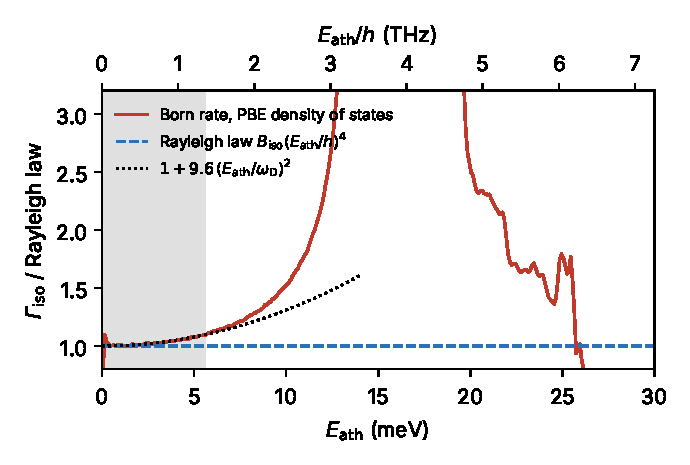
\includegraphics[width=0.75\linewidth]{figures/ch20/limit20_2b.pdf}
\captionof{figure}{Isotope scattering rate of silicon from the Born rate \cref{eq:20.2-isoborn} with the full density of states (red), divided by the Rayleigh law \cref{eq:20.2-rayleigh} (dashed, one), against the phonon energy (lower axis) and frequency (upper axis). The ratio is $g_{\mathrm{ph},\kappa}(\omega)/g_{\mathrm{Debye}}(\omega)$, independent of the mass variance. Density of states from the PBE force constants of \cref{sec:5.2}, integrated in spherical coordinates about $\mathrm{\Gamma}$ to the zone boundary (32 Gauss--Legendre polar points, 64 azimuths, 800 radial steps, \SI{0.1}{meV} bins, running mean over three bins); the Debye reference uses the PBE sound speeds. Dotted: the leading correction $1 + 9.6\,(E_{\mathrm{ath}}/\omega_{\mathrm{D}})^2$, fitted between 2 and \SI{6}{meV}, with $\omega_{\mathrm{D}} = \SI{55.6}{meV}$. Gray: within \SI{10}{\percent} of the Rayleigh law, $E_{\mathrm{ath}} \le \SI{5.6}{meV}$. The ratio peaks at 8.1 near \SI{17.6}{meV}, above the plotted range.}\label{fig:20-limit-iso}
\par}
\smallskip
Above \SI{1.4}{THz} the transverse branches of silicon are no longer linear, and the rate follows the density of states rather than the fourth power of the frequency.
\end{limitbox}

\subsection{The scaling spectrum}\label{sec:20.2-scaling}

The two rates set up a hierarchy. For a longitudinal phonon their ratio is $B_{\mathrm{iso}}/A_{\mathrm{anh}}$ divided by the frequency, and $B_{\mathrm{iso}}/A_{\mathrm{anh}}$ is \SI{33}{THz} in silicon and \SI{228}{THz} in germanium with its slowest decay. A phonon scatters off isotopes more often than it decays, by a factor 3.3 at \SI{10}{THz} in silicon and by more at lower frequency. Between two decays the branches stay close to their equilibrium shares, and a phonon of any branch spends the fraction $f_{\mathrm{LA}}$ of its time as a longitudinal phonon, the only branch that decays. The population decays at the mean rate $f_{\mathrm{LA}}\varGamma_{\mathrm{anh}}$, and isotope scattering, which conserves energy, drops out of the evolution of the energy spectrum. Let $\rho_E(E_{\mathrm{ath}}, t)$ be the energy per unit phonon energy, and $P_{\mathrm{d}}(y)$ the energy-weighted distribution of the fraction $y$ that a decay passes to a daughter, counting both daughters: with $p(y)$ the number density of one daughter, $P_{\mathrm{d}}(y) = 2y\,p(y)$, so that $\int_0^1P_{\mathrm{d}}(y)\,\dd y = 1$. Energy flows only downward:
\begin{equation}
  \frac{\partial\rho_E(E,t)}{\partial t} = -f_{\mathrm{LA}}\varGamma_{\mathrm{anh}}(E)\,\rho_E(E,t)
  + \int_E^\infty\frac{\dd E'}{E'}\,P_{\mathrm{d}}\Bigl(\frac{E}{E'}\Bigr)\,f_{\mathrm{LA}}\varGamma_{\mathrm{anh}}(E')\,\rho_E(E',t) .
  \label{eq:20.2-frag}
\end{equation}
In the isotropic continuum $P_{\mathrm{d}}$ depends on the energy ratio alone, as the distribution of \cref{app:E.12} does, since the kinematics of a decay contain no energy scale. The rate \cref{eq:20.2-anh} contains one scale, which combines with the time into
\begin{equation}
  E_*(t) = h\,(f_{\mathrm{LA}}A_{\mathrm{anh}}t)^{-1/5} , \qquad
  f_{\mathrm{LA}}\varGamma_{\mathrm{anh}}(E) = \frac{1}{t}\Bigl(\frac{E}{E_*(t)}\Bigr)^5 .
  \label{eq:20.2-Estar}
\end{equation}
A phonon above $E_*(t)$ has had time to decay, and one below it has not. Since $E_*$ is the only energy scale, we look for a solution that depends on the phonon energy only through $y = E/E_*(t)$ and conserves the total energy.
\begin{keyresult}[Scaling spectrum of down-conversion]
\begin{equation}
  \begin{gathered}
  \rho_E(E_{\mathrm{ath}}, t) = \frac{E_{\mathrm{prompt}}}{E_*(t)}\,\varphi_*\Bigl(\frac{E_{\mathrm{ath}}}{E_*(t)}\Bigr) , \\
  \frac15\,\frac{\dd}{\dd y}\bigl[y\varphi_*(y)\bigr] = -y^5\varphi_*(y) + \int_y^\infty\dd y'\,y'^4P_{\mathrm{d}}\Bigl(\frac{y}{y'}\Bigr)\varphi_*(y') ,
  \end{gathered}
  \label{eq:20.2-scaling}
\end{equation}
with $\int\varphi_*\,\dd y = 1$. The spectrum keeps its shape and slides to lower energy as $t^{-1/5}$, and every energy moment scales with $E_*(t)$.
\end{keyresult}
\noindent Inserting the form into \cref{eq:20.2-frag} gives the equation for $\varphi_*$. Since $\dd E_*/\dd t = -E_*/5t$, the time derivative of $\rho_E$ is $(E_{\mathrm{prompt}}/5tE_*)\,\dd(y\varphi_*)/\dd y$. The loss term is $(E_{\mathrm{prompt}}/tE_*)\,y^5\varphi_*$ by \cref{eq:20.2-Estar}, and the gain term becomes the integral after the substitution $E' = E_*y'$. Every term carries the factor $E_{\mathrm{prompt}}/tE_*$, so the time drops out. Integrating over $y$ checks the energy: the left side gives $[y\varphi_*]_0^\infty = 0$, and the two terms on the right cancel after the order of integration is exchanged, since $\int_0^{y'}P_{\mathrm{d}}(y/y')\,\dd y = y'$.

\Cref{eq:20.2-scaling} says what the spectrum looks like once it has settled, not when it settles. Settling needs a time long compared with the first decay of the hardest phonons, $1/(f_{\mathrm{LA}}A_{\mathrm{anh}}f_{\mathrm{top}}^5)$ for a band top $f_{\mathrm{top}}$. This is \SI{0.19}{ns} in silicon ($f_{\mathrm{top}} = \SI{15}{THz}$, $f_{\mathrm{LA}} = 0.093$) and \SI{1.3}{ns} in germanium ($f_{\mathrm{top}} = \SI{8.64}{THz}$, $f_{\mathrm{LA}} = 0.098$, $A_{\mathrm{anh}} = \SI{1.61e-55}{s^4}$). Settling also needs the hierarchy of rates, the fifth-power law, and no absorption or surface scattering in the meantime. In silicon the scale is $E_*(t) = 44.6$, 28.1, 17.7 and \SI{11.2}{meV} at 1, 10 and \SI{100}{ns} and \SI{1}{\micro s}, and in germanium 37.8, 23.8, 15.0 and \SI{9.5}{meV}. Since $E_* \propto A_{\mathrm{anh}}^{-1/5}$, the factor of ten among the germanium constants moves $E_*$ by a factor 0.63, and the factor 1.55 between the two silicon values moves it by 0.92.

We have no proof that every birth spectrum approaches $\varphi_*$, which is a question about the stability of \cref{eq:20.2-scaling}; we solve \cref{eq:20.2-frag} for representative births instead. For $P_{\mathrm{d}}$ we take a symmetric stand-in for the isotropic-continuum distribution: each daughter receives a fraction $y$ drawn from the beta distribution $30y^2(1 - y)^2$, which gives $P_{\mathrm{d}}(y) = 60\,y^3(1 - y)^2$. On a logarithmic energy grid of step 0.01, \cref{eq:20.2-frag} becomes a linear system whose exponential we compute exactly. The settled spectrum has its energy-weighted median at $0.66\,E_*$ and \SI{80}{\percent} of its energy between $0.36\,E_*$ and $0.97\,E_*$, and its mean is $\langle E_{\mathrm{ath}}\rangle = 0.667\,E_*(t)$. \Cref{lim:20.2a} follows the mean energy of three hard births in silicon: a line at the band top, a spectrum that grows as the cube of the energy up to the band top, and the acoustic pairs of optical decay. The cubic spectrum puts equal energy in every mode of the Debye model, the shape of a locally thermalized recoil. All three reach the scaling law within \SI{10}{\percent} after \SI{0.46}{ns}, a few first-decay times.

\begin{limitbox}[Down-conversion and the scaling spectrum][lim:20.2a]
The published rates are $\varGamma_{\mathrm{anh}} = A\nu^5$ for longitudinal phonons and $\varGamma_{\mathrm{iso}} = B\nu^4$ for all branches~\cite[Eqs.~(6), (8)]{leman2012invited}, with $A = \SI{7.41e-56}{s^4}$ and $B = \SI{2.43e-42}{s^3}$ for silicon~\cite[Table~I]{leman2012invited}. With the mode mixing of Kelsey et al.~\cite[Sect.~2.2.2]{kelsey2023g4cmp} they imply the scaling spectrum \cref{eq:20.2-scaling}, $E_* \propto t^{-1/5}$, and the mean energy $\langle E_{\mathrm{ath}}\rangle = 0.667\,E_*(t)$ for the daughter distribution used here.
\par\smallskip
{\centering
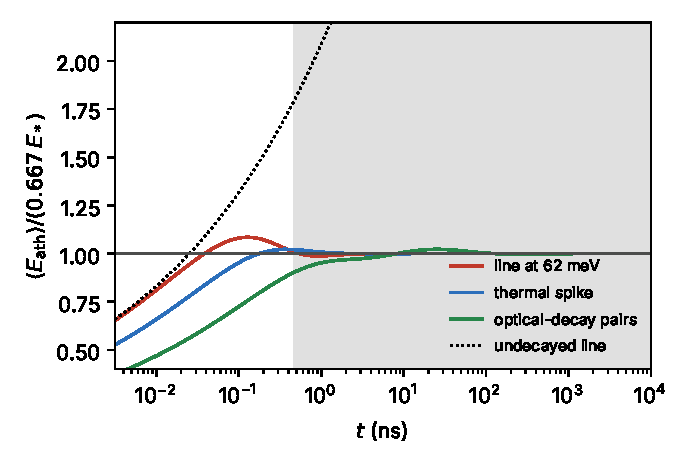
\includegraphics[width=0.75\linewidth]{figures/ch20/limit20_2a.pdf}
\captionof{figure}{Energy-weighted mean phonon energy in silicon divided by the scaling law $0.667\,E_*(t)$ of \cref{eq:20.2-Estar,eq:20.2-scaling}, against time, for three hard births (models): a line at the band top, \SI{62}{meV} (red); a spectrum growing as $E_{\mathrm{ath}}^3$ up to \SI{62}{meV} (blue); and the pairs of longitudinal (\SI{42}{meV}) and transverse (\SI{22}{meV}) phonons from optical decay, Gaussians of \SI{10}{\percent} relative width (green). Solution of \cref{eq:20.2-frag} with $f_{\mathrm{LA}} = 0.093$, $A_{\mathrm{anh}} = \SI{7.41e-56}{s^4}$, the daughter distribution $P_{\mathrm{d}}(y) = 60\,y^3(1 - y)^2$ and no surfaces, on a logarithmic grid of step 0.01 from 0.01 to \SI{18}{THz}, by the exact matrix exponential. Dotted: the leading correction at early times, the undecayed line, $(f_{\mathrm{LA}}A_{\mathrm{anh}}f_{\mathrm{top}}^5t)^{1/5}/0.667$. Gray: all three within \SI{10}{\percent}, $t \ge \SI{0.46}{ns}$.}\label{fig:20-limit-scaling}
\par}
\smallskip
Before the hardest phonons have decayed a few times the mean still depends on the birth spectrum; and where the continuum rates fail, above a few THz in silicon (\cref{lim:20.2b}), the time scale itself is an estimate.
\end{limitbox}

\subsection{Memory of the birth spectrum}\label{sec:20.2-memory}

How long does the birth spectrum leave a trace? We measure the trace by the total-variation distance between the normalized energy spectra that two births reach at time $t$, which is half the integral of their absolute difference. It bounds the difference of the energy that the two deliver into any part of the spectrum. Let $\Delta_{\mathrm{h}}(t)$ be its largest value over pairs of births above an energy $E_{\mathrm{mem}}$. By the scaling form $\Delta_{\mathrm{h}}$ depends on time only through $E_*(t)/E_{\mathrm{mem}}$, and the solutions of \cref{eq:20.2-frag} give the threshold: any two births above $E_{\mathrm{mem}}$ agree to $10^{-3}$ once $E_*(t)$ has fallen to between 0.51 and $0.53\,E_{\mathrm{mem}}$. A birth is forgotten when the scale has fallen to about half its energy, and since $E_* \propto t^{-1/5}$ the time this takes grows as the inverse fifth power of the birth energy. \Cref{fig:20-spectrum} shows the consequences for silicon.

\begin{figure}[tbp]
  \centering
  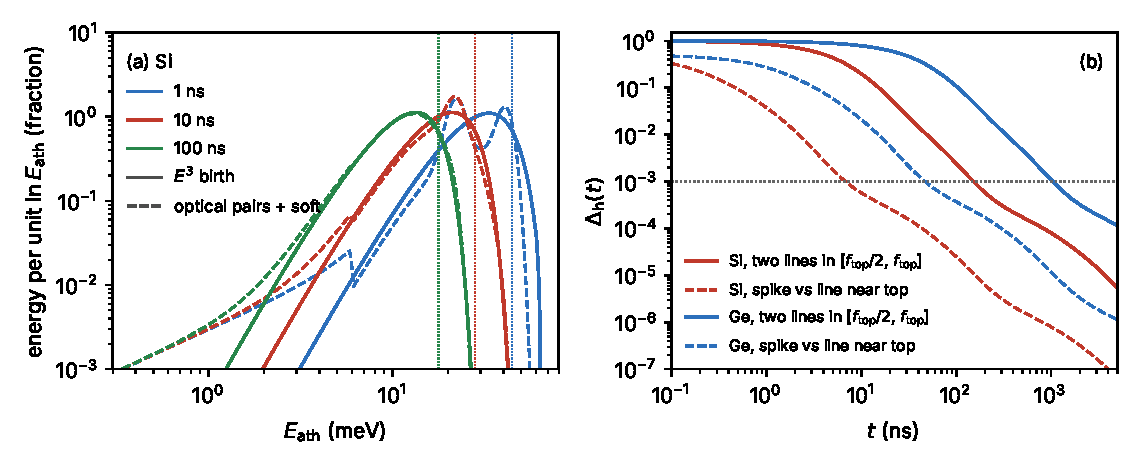
\includegraphics[width=\linewidth]{figures/ch20/fig20_2.pdf}
  \caption{Down-conversion of prompt phonons, from \cref{eq:20.2-frag} in the isotropic continuum with the mean decay rate $f_{\mathrm{LA}}A_{\mathrm{anh}}(E_{\mathrm{ath}}/h)^5$ for every phonon, the daughter distribution $P_{\mathrm{d}}(y) = 60\,y^3(1 - y)^2$ and no surfaces. (a) Energy spectrum of a silicon event, per unit $\ln E_{\mathrm{ath}}$ and normalized to the prompt energy, at 1, 10 and \SI{100}{ns} (colors), for two births (models). Solid: a spectrum growing as $E_{\mathrm{ath}}^3$ up to the band top, \SI{62}{meV}, standing for a locally thermalized nuclear recoil. Dashed: the longitudinal (\SI{42}{meV}) and transverse (\SI{22}{meV}) phonons of optical decay, Gaussians of \SI{10}{\percent} relative width with the energy shares 42:22 of the two phonons of an optical decay, plus the soft fraction $f_{\mathrm{s}} = \SI{1.7}{\percent}$ spread uniformly in energy over 0.2 to \SI{6}{meV}, standing for an electron recoil. Dotted verticals: $E_*(t)$. $A_{\mathrm{anh}} = \SI{7.41e-56}{s^4}$, $f_{\mathrm{LA}} = 0.093$. (b) Memory of the hard part, $\Delta_{\mathrm{h}}(t)$, for silicon (red) and germanium (blue; $A_{\mathrm{anh}} = \SI{1.61e-55}{s^4}$, $f_{\mathrm{LA}} = 0.098$, band top \SI{8.64}{THz}). Solid: the largest total-variation distance between two line births in the upper factor two of the band, $[f_{\mathrm{top}}/2, f_{\mathrm{top}}]$ (six lines). Dashed: one pair concentrated near the top, the $E_{\mathrm{ath}}^3$ spectrum against a Gaussian line at $0.95\,f_{\mathrm{top}}$ of width $0.05\,f_{\mathrm{top}}$. Dotted: $10^{-3}$, crossed by the dashed curves at \SI{6.8}{ns} (Si) and \SI{47}{ns} (Ge), and by the solid curves at \SI{0.15}{\micro s} (Si) and \SI{1.0}{\micro s} (Ge).}
  \label{fig:20-spectrum}
\end{figure}

The answer depends on how low the hard births reach. Take two births concentrated at the top of the band, the cubic spectrum and a line at \SI{95}{\percent} of the band top. They agree to $10^{-3}$ after \SI{6.8}{ns} in silicon and \SI{47}{ns} in germanium with its slowest decay constant (\cref{fig:20-spectrum}(b)), and the fastest germanium constant shortens the latter tenfold. Births spread over the upper factor two of the band take longer, \SI{0.15}{\micro s} in silicon and \SI{1.0}{\micro s} in germanium. The transverse phonons of optical decay, at \SI{22}{meV}, are forgotten only when $E_*$ has fallen to about \SI{11}{meV}, near \SI{1}{\micro s} in silicon. The two model births of \cref{fig:20-spectrum}(a) differ by a total-variation distance of 0.13 at \SI{10}{ns}, 0.026 at \SI{100}{ns}, 0.015 at \SI{300}{ns} and 0.012 at \SI{1}{\micro s}. At \SI{1}{\micro s} their parts above \SI{6}{meV} agree to $6\times10^{-4}$. What remains is the soft fraction: the electron recoil was born with \SI{1.7}{\percent} of its energy below \SI{6}{meV} and the cubic spectrum with \SI{0.01}{\percent}, and the decay of the hard parts has only begun to fill that region. All of these times rest on the continuum rates, which in silicon are applied at 5 to \SI{15}{THz}, above their range (\cref{lim:20.2b}), so they are estimates.

Polarization is forgotten much sooner. Along the scaling trajectory, the number of times a phonon has scattered off isotopes by the time $t$ is
\begin{equation}
  N_{\mathrm{mix}}(t) = \int_0^t\dd t'\,B_{\mathrm{iso}}\bigl[E_*(t')/h\bigr]^4 = 5B_{\mathrm{iso}}\,(f_{\mathrm{LA}}A_{\mathrm{anh}})^{-4/5}\,t^{1/5} ,
  \label{eq:20.2-Nmix}
\end{equation}
which is 164 at \SI{1}{ns} in silicon and 650 at \SI{1}{\micro s}; in germanium, with fifteen times the isotope constant, it is \num{1300} and \num{5100}. Each scattering redraws the branch from the equilibrium shares, so the fraction of phonons that still carry their birth branch is of order $\ee^{-N_{\mathrm{mix}}}$.

The phonons also spread out. Take the diffusion constant $v_{\mathrm{ph}}^2/3\varGamma_{\mathrm{iso}}$ of a gas with mean free time $1/\varGamma_{\mathrm{iso}}$ and rms group speed $v_{\mathrm{ph}}$, evaluated at $E_*(t)$. The mean squared distance from the event is then $6\int\dd t'\,v_{\mathrm{ph}}^2/3\varGamma_{\mathrm{iso}} = \frac{10}{9}v_{\mathrm{ph}}^2(f_{\mathrm{LA}}A_{\mathrm{anh}})^{4/5}t^{9/5}/B_{\mathrm{iso}}$. In silicon, with $v_{\mathrm{ph}} = \SI{5.85}{km/s}$, the rms distance is \SI{8.6}{\micro m} at \SI{10}{ns}, \SI{68}{\micro m} at \SI{100}{ns} and \SI{0.54}{mm} at \SI{1}{\micro s}. In germanium, with $v_{\mathrm{ph}} = \SI{3.52}{km/s}$, it is \SI{1.8}{\micro m}, \SI{15}{\micro m} and \SI{0.12}{mm}. This is the quasi-diffuse transport of athermal phonons~\cite[Sect.~2.2.2]{kelsey2023g4cmp}: the phonons random-walk while their mean free path grows with each decay, until it reaches the size of the crystal and they move ballistically. A phonon of \SI{45}{meV}, the binding energy of a phosphorus donor, belongs to a population that decays within \SI{0.95}{ns}, by which time it has spread over \SI{1.0}{\micro m}. An event closer to a sensor than the rms distance delivers part of its energy before its spectrum has settled, and there the birth is not forgotten. For a silicon detector \SI{4}{mm} thick with sensors on one face, such as that of Ren et al.~\cite{ren2021design}, that shell is \SI{0.21}{\percent} of the volume at \SI{10}{ns}, \SI{1.7}{\percent} at \SI{100}{ns} and \SI{13.5}{\percent} at \SI{1}{\micro s}. The memory times above decide how much of the volume counts as bulk.

Sapphire does not fit this picture. Its isotope constant is a hundred times smaller than that of silicon, $B_{\mathrm{iso}} = \SI{2.5e-44}{s^3}$ calculated and \SI{4e-44}{s^3} measured, while its decay constant lies between \num{1.88e-55} and \SI{1.27e-54}{s^4}. Hernandez et al.\ trace that spread to the anisotropy and to converting a published rate with the fifth power of a sound speed~\cite[Tables~3, 4]{hernandez2025modeling}. Compared to silicon, however, the hierarchy is reversed: mixing outpaces decay only below $B_{\mathrm{iso}}/A_{\mathrm{anh}} = 0.02$ to \SI{0.21}{THz}. Over the whole primary band a longitudinal phonon decays before it scatters, and the branches are not held at their equilibrium shares. A transverse phonon, which the isotropic continuum does not let decay, scatters $B_{\mathrm{iso}}(E_{\mathrm{ath}}/h)^4\times\SI{1}{\micro s} = 0.025$, 0.4 and 16 times in a microsecond at 1, 2 and \SI{5}{THz}. As a result, transverse phonons born below a few THz in sapphire keep their energy and their polarization for microseconds. The single rate $f_{\mathrm{LA}}\varGamma_{\mathrm{anh}}$ of \cref{eq:20.2-frag} does not exist, and the scaling argument fails at its first step. The fate of these phonons needs the decay rates of transverse phonons in an anisotropic crystal, which the isotropic continuum sets to zero.

\subsection{Transfer-kernel bound on observable differences}\label{sec:20.2-bound}

The memory of the spectrum matters through what a readout measures. Take an observable that is linear in the energies delivered to the sensors, with weights between zero and one: the fraction of the energy absorbed by one of two sensors, the fraction that arrives before a given time, or the collection efficiency of a population. Since the transport is linear, a birth spectrum $\hat\rho_0(E)$ normalized to unit energy gives $O = \int\dd E\,R_O(E)\,\hat\rho_0(E)$. Here $R_O(E)$, with $0 \le R_O \le 1$, is the value of the observable for unit energy born at $E$ at the event position, and \cref{sec:20.5} builds it from the collection kernels of a detector. Let $\Delta\hat\rho_0 = \hat\rho_0^{\mathrm{NR}} - \hat\rho_0^{\mathrm{ER}}$ be the difference of the birth spectra of the two recoils. Suppose that no sensor absorbs anything before a time $t_{\mathrm{mem}}$, and that births above $E_{\mathrm{mem}}$ have been forgotten by then, to the distance $\Delta_{\mathrm{h}}(t_{\mathrm{mem}})$ in energy, branch and position.
\begin{keyresult}[Transfer-kernel bound]
\begin{equation}
  |O^{\mathrm{NR}} - O^{\mathrm{ER}}| \le \int_0^{E_{\mathrm{mem}}}\dd E\,|\Delta\hat\rho_0(E)| + \Delta_{\mathrm{h}}(t_{\mathrm{mem}}) .
  \label{eq:20.2-bound}
\end{equation}
When $\Delta\hat\rho_0$ has one sign below $E_{\mathrm{mem}}$, the integral is $\Delta_{\mathrm{soft}} = |\int_0^{E_{\mathrm{mem}}}\Delta\hat\rho_0\,\dd E|$, the difference of the energy fractions born below $E_{\mathrm{mem}}$.
\end{keyresult}
\noindent The response to a birth above $E_{\mathrm{mem}}$ is the response to the state it has reached at $t_{\mathrm{mem}}$, and a weight between zero and one integrated against the difference of two normalized distributions is bounded by their total-variation distance. Two births $E_1$, $E_2$ above $E_{\mathrm{mem}}$ therefore have $|R_O(E_1) - R_O(E_2)| \le \Delta_{\mathrm{h}}$. Both birth spectra have unit energy, so $\int\Delta\hat\rho_0\,\dd E = 0$ and $O^{\mathrm{NR}} - O^{\mathrm{ER}} = \int(R_O - R_0)\,\Delta\hat\rho_0\,\dd E$ for any constant $R_0$. Choose $R_0$ midway between the largest and the smallest response above $E_{\mathrm{mem}}$. Then $|R_O - R_0| \le \Delta_{\mathrm{h}}/2$ above $E_{\mathrm{mem}}$, where $\int|\Delta\hat\rho_0| \le 2$, and $|R_O - R_0| \le 1$ below, which gives the two terms of \cref{eq:20.2-bound}. An observable that is a ratio of delivered energies, such as the share of one of two sensors, is linear to first order in the difference, and the range of its linearized weight replaces the factor one.

\Cref{eq:20.2-bound} names the one number that the created-phonon spectra of the two recoils must supply, the distance between their parts below $E_{\mathrm{mem}}$. The single-sign condition matters. Two births with the same energy below $E_{\mathrm{mem}}$ but different soft shapes, one just above the gap of a sensor film and one just below it, have $\Delta_{\mathrm{soft}} = 0$ and yet give different responses; the bound then needs the full $L^1$ distance. The branch content of a nuclear recoil above $E_{\mathrm{mem}}$ does not enter at all.

For the primary phonons the bound limits the spectral part of the collection offset of \cref{sec:19.5}. With the collection efficiency as the observable, $|\epsilon^{\mathrm{NR}}_{\mathrm{prim}} - \epsilon^{\mathrm{ER}}_{\mathrm{prim}}| \le \int_0^{E_{\mathrm{mem}}}|\Delta\hat\rho_0| + \Delta_{\mathrm{h}}$. If $E_{\mathrm{mem}}$ lies above the soft band and below every hard birth, and only the electron recoil carries a soft fraction, the integral is $f_{\mathrm{s}} = \SI{1.7}{\percent}$. The condition on $E_{\mathrm{mem}}$ is the weak point. For the model births of \cref{fig:20-spectrum}(a) at \SI{1}{\micro s}, the lowest energy above which births agree to $10^{-3}$, $E_{\mathrm{mem}} = \SI{21.6}{meV}$, cuts through the transverse daughters of optical decay, and the bound is 0.15, against an actual largest difference of 0.012. At \SI{3}{\micro s}, with $E_{\mathrm{mem}} = \SI{17.7}{meV}$, the bound has fallen to 0.026 against 0.009, but the near-face shell of a \SI{4}{mm} crystal is by then \SI{36}{\percent} of the volume. Within the bulk the spectral difference between the two recoils is set by the soft fraction and by how low the hard births reach; near an instrumented face this argument does not bound it.

\section{Phonons into films}\label{sec:20.3}

A phonon that has down-converted in silicon to about a terahertz (\cref{sec:20.2}) reaches an aluminum film \SI{60}{nm} thick on the crystal surface. Silicon and aluminum have almost the same acoustic impedance, and the normal-incidence law of \cref{app:C.18} lets \SI{99}{\percent} of a longitudinal flux through. A fit of measured pulses with a phonon simulation nevertheless returns a silicon-to-aluminum coefficient of 0.3 to 0.55 for such a film~\cite{martinez2019measurements}, and a phonon inside the film that reaches the interface crosses back into the silicon about once in three arrivals. These three numbers measure different things. The transmission of each polarization at every angle, and the reciprocity that ties the two directions together, explain all three, and from them follow the probability that a phonon entering the film is absorbed there and the time $t_l$ it spends in the film before escaping, which controls the quasiparticle yield of \cref{sec:20.4}.

\subsection{Acoustic mismatch at oblique incidence}\label{sec:20.3-amm}

The acoustic mismatch model treats the interface as a welded plane between two elastic continua: displacement and traction are continuous across it, and nothing else happens there~\cite{swartz1989thermal}. Silicon is cubic, with an anisotropy ratio $2C_{44}/(C_{11} - C_{12}) = 1.56$ (\cref{app:C.18}). Aluminum is nearly isotropic: its elastic constants extrapolated to zero temperature, $C_{11} = 114.3$, $C_{12} = 61.9$ and $C_{44} = \SI{31.6}{GPa}$~\cite[Table~2]{malica2020quasi}, give the ratio 1.21. We replace each crystal by an isotropic medium with the Voigt averages of its elastic constants, the bulk modulus $B$ of \cref{eq:C.18-bulk} and the shear modulus $(C_{11} - C_{12} + 3C_{44})/5$, which is also what transport codes do. Silicon then has the speeds $c_{\mathrm{LA}} = \SI{9.00}{km.s^{-1}}$ and $c_{\mathrm{T}} = \SI{5.40}{km.s^{-1}}$ at $\rho_T = \SI{2.33}{g.cm^{-3}}$, and aluminum $c_{\mathrm{LA}} = \SI{6.63}{km.s^{-1}}$ and $c_{\mathrm{T}} = \SI{3.30}{km.s^{-1}}$ at the room-temperature density \SI{2.70}{g.cm^{-3}}. A subscript 1 or 2 on a speed or density names the medium.

Put the interface at $z = 0$, with medium 1 below it. A plane wave of frequency $\omega$ that arrives from medium 1 at the angle $\theta_1$ to the normal has the wavevector component $Q_\parallel = \omega\sin\theta_1/c_{\mathrm{inc}}$ along the interface, where $c_{\mathrm{inc}}$ is its speed. Every reflected and transmitted wave it generates has the same $\omega$ and the same $Q_\parallel$, which is the acoustic Snell law \cref{eq:C.18-snell}. A wave of speed $c$ in either medium then has the normal component
\begin{equation}
  Q_z = \bigl(\omega^2/c^2 - Q_\parallel^2\bigr)^{1/2} ,
  \label{eq:20.3-Qz}
\end{equation}
taken positive. When $Q_\parallel > \omega/c$ the root is imaginary, we take it with a positive imaginary part, and the wave decays away from the interface and carries no energy flux. A wave can have three polarizations: longitudinal (L), transverse in the plane of incidence (SV), and transverse perpendicular to it (SH). The interface is invariant under reflection through the plane of incidence, so SH waves couple only to SH waves, while L and SV waves mix.

For SH waves the displacement $u_y$ and the traction $\sigma_{yz} = \rho_Tc_{\mathrm{T}}^2\,\partial_zu_y$ must be continuous. This is the algebra of the normal-incidence derivation in \cref{app:C.18}, with $Q_i\rho_ic_i^2$ there replaced by $\rho_ic_{\mathrm{T},i}^2Q_{z,i} = \omega Z^{\mathrm{T}}_{\mathrm{ac},i}\cos\theta_i$, where $Z^{\mathrm{T}}_{\mathrm{ac},i} = \rho_ic_{\mathrm{T},i}$ is the transverse impedance. The fraction of the incident energy flux that crosses is
\begin{equation}
  t_{\mathrm{SH}}(\theta_1) = \frac{4Z^{\mathrm{T}}_{\mathrm{ac},1}\cos\theta_1\,\Real\bigl(Z^{\mathrm{T}}_{\mathrm{ac},2}\cos\theta_2\bigr)}{\bigl|Z^{\mathrm{T}}_{\mathrm{ac},1}\cos\theta_1 + Z^{\mathrm{T}}_{\mathrm{ac},2}\cos\theta_2\bigr|^2} ,
  \qquad
  \cos\theta_2 = \Bigl(1 - \frac{c_{\mathrm{T},2}^2}{c_{\mathrm{T},1}^2}\sin^2\theta_1\Bigr)^{1/2} .
  \label{eq:20.3-SH}
\end{equation}
At normal incidence it is \cref{eq:C.18-transmission} with the transverse impedances. Beyond the critical angle $\sin\theta_1 = c_{\mathrm{T},1}/c_{\mathrm{T},2}$, which exists when medium 2 is the faster one, $\cos\theta_2$ is imaginary and $t_{\mathrm{SH}} = 0$: the wave is totally reflected.

For L and SV waves four conditions hold at $z = 0$: continuity of $u_x$, $u_z$, $\sigma_{zz} = \rho_T[c_{\mathrm{LA}}^2\partial_zu_z + (c_{\mathrm{LA}}^2 - 2c_{\mathrm{T}}^2)\partial_xu_x]$ and $\sigma_{xz} = \rho_Tc_{\mathrm{T}}^2(\partial_zu_x + \partial_xu_z)$, the last two being Hooke's law of \cref{app:C.18} for an isotropic medium. Each wave is $u = a\,\hat{\vect{e}}\,\ee^{\ii(Q_\parallel x \pm Q_zz - \omega t)}$ with amplitude $a$ and the sign $+$ for a wave moving toward medium 2 and $-$ for one moving back into medium 1, and unit polarization $\hat{\vect{e}} = (c/\omega)(Q_\parallel, 0, \pm Q_z)$ for L and $(c/\omega)(\pm Q_z, 0, -Q_\parallel)$ for SV. Collect for each wave the four quantities that must match,
\begin{equation}
  \vect{b} = \Bigl(\hat e_x,\ \hat e_z,\ \frac{\rho_T}{\omega}\bigl[c_{\mathrm{LA}}^2(\pm Q_z)\hat e_z + (c_{\mathrm{LA}}^2 - 2c_{\mathrm{T}}^2)Q_\parallel\hat e_x\bigr],\ \frac{\rho_Tc_{\mathrm{T}}^2}{\omega}\bigl[(\pm Q_z)\hat e_x + Q_\parallel\hat e_z\bigr]\Bigr) ,
  \label{eq:20.3-b}
\end{equation}
which are the displacement and $\sigma_{zz}/\ii\omega$, $\sigma_{xz}/\ii\omega$ per unit amplitude. With unit incident amplitude the boundary conditions read $\vect{b}_{\mathrm{inc}} + a_{\mathrm{rL}}\vect{b}_{\mathrm{rL}} + a_{\mathrm{rS}}\vect{b}_{\mathrm{rS}} = a_{\mathrm{tL}}\vect{b}_{\mathrm{tL}} + a_{\mathrm{tS}}\vect{b}_{\mathrm{tS}}$, four linear equations for the amplitudes of the reflected (r) and transmitted (t) L and SV waves. A propagating plane wave carries the time-averaged energy flux $\frac12\rho_T\omega^2|a|^2c$ along its direction (\cref{app:C.18}), whose normal component is this times $\cos\theta = cQ_z/\omega$. The fraction of the incident flux carried away by the outgoing wave $j$ is therefore
\begin{equation}
  t_j = \frac{\rho_jc_j^2\,\Real Q_{z,j}\,|a_j|^2}{\rho_1c_{\mathrm{inc}}^2\,Q_{z,\mathrm{inc}}} ,
  \label{eq:20.3-flux}
\end{equation}
and the transmission of an incident L or SV wave is the sum of the two transmitted fractions. We solve the four equations numerically at each angle.

\Cref{fig:20-amm} shows the result for silicon and aluminum. From the silicon side, a longitudinal phonon crosses with 0.99 at normal incidence and with more than 0.98 out to \SI{70}{\degree}, falling below 0.9 only beyond \SI{78}{\degree}. At oblique incidence part of the transmitted flux is converted to SV, \num{0.031} at \SI{30}{\degree} and at most 0.17, near \SI{76}{\degree}. Transverse phonons cross with 0.97 at normal incidence. The one critical angle that limits transmission from silicon is \SI{54.6}{\degree}, beyond which an incident SV wave can no longer produce a longitudinal wave in aluminum. From the aluminum side, however, every wave is slower than every wave in silicon, and the critical angles cut transmission off. Transverse phonons beyond $\arcsin(c_{\mathrm{T,Al}}/c_{\mathrm{T,Si}}) = \SI{37.7}{\degree}$ find no propagating wave in silicon and are totally reflected. Longitudinal phonons lose the longitudinal channel beyond \SI{47.5}{\degree} and keep only the conversion into silicon transverse waves, which carries 0.28 at that angle and vanishes at grazing incidence.

\begin{figure}[tbp]
  \centering
  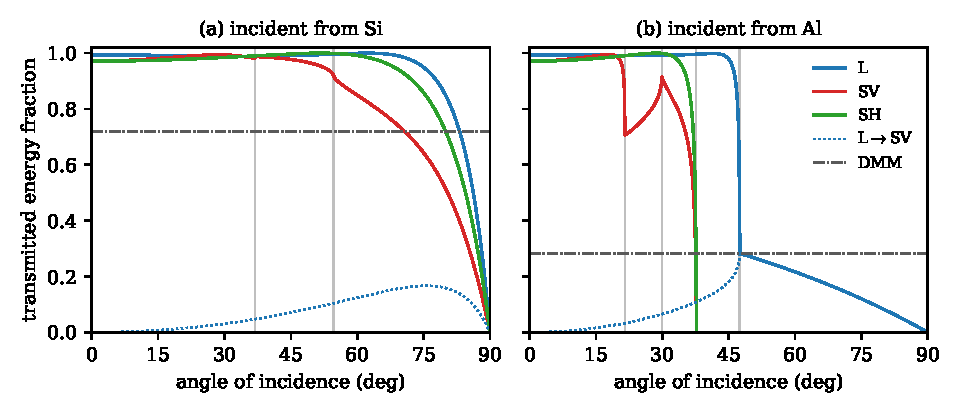
\includegraphics[width=\linewidth]{figures/ch20/fig20_3.pdf}
  \caption{Acoustic-mismatch transmission of a welded silicon/aluminum interface against the angle of incidence, for phonons incident (a) from silicon and (b) from aluminum. Solid: fraction of the incident energy flux transmitted into all modes of the other side, for incident longitudinal (L, blue), SV (red) and SH (green) phonons; dotted: the part of the incident longitudinal flux transmitted as SV. Dash-dot: the diffuse-mismatch value $\mathfrak{n}_2/(\mathfrak{n}_1 + \mathfrak{n}_2)$, 0.718 in (a) and 0.282 in (b). Gray lines: critical angles, \SI{36.9}{\degree} and \SI{54.6}{\degree} in (a); \SI{21.5}{\degree}, \SI{29.9}{\degree}, \SI{37.7}{\degree} and \SI{47.5}{\degree} in (b). Both media isotropic, with the Voigt averages of the elastic constants: silicon (\cref{app:C.18}) $c_{\mathrm{LA}} = 9.00$, $c_{\mathrm{T}} = \SI{5.40}{km.s^{-1}}$, $\rho_T = \SI{2.33}{g.cm^{-3}}$; aluminum, zero-temperature elastic constants at the room-temperature density, 6.63, \SI{3.30}{km.s^{-1}}, \SI{2.70}{g.cm^{-3}}. The curves do not depend on frequency.}
  \label{fig:20-amm}
\end{figure}

Frequency drops out of \cref{eq:20.3-SH,eq:20.3-flux}, because $Q_\parallel$ and $Q_z$ both scale with $\omega$. The transmissions are frequency independent as long as the wavelength is long compared with the lattice spacing, so that the continuum holds, and short compared with the film thickness, so that the film acts as a half-space. In the simulation of the \SI{60}{nm} films the absorbed phonons peak between 0.7 and \SI{0.9}{THz}~\cite[Sect.~V]{martinez2019measurements}. At \SI{0.8}{THz} the wavelengths in aluminum are \SI{8.3}{nm} for longitudinal and \SI{4.1}{nm} for transverse phonons, so both conditions hold. The longitudinal wavelength equals the thickness at \SI{0.110}{THz}, close to the pair-breaking threshold $2\Delta_{\mathrm{BCS}} = \SI{0.36}{meV}$, or \SI{0.087}{THz}, of bulk aluminum (\cref{sec:7.2}); below it the film reflects as a layer, with interference between its two faces.

\subsection{Angle averages, reciprocity and diffuse mismatch}\label{sec:20.3-recip}

A sensor film collects phonons arriving from all directions, so its transmission is the average over an isotropic population. Count the energy flux that such a population sends onto unit area of the interface. A branch has $\dd^3Q/(2\pi)^3$ modes in $\dd^3Q$, each with occupation $n(\omega)$, energy $\omega$ and normal group velocity $\partial\omega/\partial Q_z$. Since $\dd Q_z\,\partial\omega/\partial Q_z = \dd\omega$, the flux is
\begin{equation}
  \int_{Q_z > 0}\frac{\dd^3Q}{(2\pi)^3}\,\omega\,n(\omega)\,\frac{\partial\omega}{\partial Q_z} = \int\dd\omega\,\omega\,n(\omega)\int\frac{\dd^2Q_\parallel}{(2\pi)^3} .
  \label{eq:20.3-count}
\end{equation}
At a given frequency, every patch $\dd^2Q_\parallel$ of every branch, in either medium, brings the same flux. In an isotropic medium $\dd^2Q_\parallel = 2\pi Q_\parallel\dd Q_\parallel = (2\pi\omega^2/c_\nu^2)\sin\theta\cos\theta\,\dd\theta$, so the angles enter with the weight $2\sin\theta\cos\theta$ and the branch $\nu$ with the weight $c_\nu^{-2}$. The mean transmission of an isotropic population from medium 1 into medium 2 is
\begin{equation}
  \bar t_{12} = \frac{1}{\mathfrak{n}_1}\sum_\nu c_{1\nu}^{-2}\int_0^{\pi/2}t_{12,\nu}(\theta)\,2\sin\theta\cos\theta\,\dd\theta ,
  \qquad
  \mathfrak{n}_1 = c_{\mathrm{LA},1}^{-2} + 2c_{\mathrm{T},1}^{-2} ,
  \label{eq:20.3-avg}
\end{equation}
where $\nu$ runs over L, SV and SH and $t_{12,\nu}(\theta)$ is the transmission of \cref{eq:20.3-SH} or \cref{eq:20.3-flux}. The interface-weighted density $\mathfrak{n}_1$ is proportional to the rate at which phonons of a given frequency strike unit area from medium 1.

Reciprocity ties the two directions together. Fix $\omega$ and $Q_\parallel$. The interface then scatters $N_1$ incoming channels from medium 1, the branches of medium 1 that propagate at this $Q_\parallel$, and $N_2$ from medium 2, into the same number of outgoing ones. Normalize each amplitude so that its squared modulus is the energy flux, as in \cref{eq:20.3-flux}. The matrix $\mathsf{S}$ that maps incoming onto outgoing amplitudes is then unitary, because the welded interface neither stores nor dissipates energy. Write it in blocks,
\begin{equation*}
  \mathsf{S} = \begin{pmatrix} \mathsf{r} & \mathsf{t}' \\ \mathsf{t} & \mathsf{r}' \end{pmatrix} ,
\end{equation*}
with $\mathsf{t}$ the $N_2\times N_1$ block of transmission from medium 1 into medium 2 and $\mathsf{t}'$ the reverse. The upper-left block of $\mathsf{S}^\dagger\mathsf{S} = 1$ gives $\mathsf{r}^\dagger\mathsf{r} + \mathsf{t}^\dagger\mathsf{t} = 1$, and that of $\mathsf{S}\mathsf{S}^\dagger = 1$ gives $\mathsf{r}\mathsf{r}^\dagger + \mathsf{t}'\mathsf{t}'^\dagger = 1$, both in the $N_1$-dimensional space of medium 1. Taking traces, $\Tr\mathsf{t}^\dagger\mathsf{t} = N_1 - \Tr\mathsf{r}^\dagger\mathsf{r} = \Tr\mathsf{t}'\mathsf{t}'^\dagger$. The left side is the sum of the transmissions of all channels incident from medium 1, the right side that of all channels incident from medium 2. Integrated over $Q_\parallel$ with the weight of \cref{eq:20.3-count}, this equality becomes a statement about the averages \cref{eq:20.3-avg}.
\begin{keyresult}[Reciprocity of interface transmission]
For any flat interface that conserves energy, the mean transmissions of isotropic populations in the two directions satisfy
\begin{equation}
  \mathfrak{n}_1\,\bar t_{12} = \mathfrak{n}_2\,\bar t_{21} .
  \label{eq:20.3-recip}
\end{equation}
\end{keyresult}
The derivation uses the conservation of $Q_\parallel$ and the conservation of energy, nothing about isotropy or the number of layers. For anisotropic media or a layered interface \cref{eq:20.3-recip} holds at each frequency, with $\mathfrak{n}_i$ replaced by the area that the branches of medium $i$ cover in the $Q_\parallel$ plane. Evanescent waves are not channels and drop out. In thermal equilibrium the relation is detailed balance: equal temperatures on the two sides give no net flux. It holds, however, for any population, since it is a property of $\mathsf{S}$.

For silicon and aluminum $\mathfrak{n}_{\mathrm{Si}} = 0.0808$ and $\mathfrak{n}_{\mathrm{Al}} = \SI{0.206}{s^2.km^{-2}}$, a ratio of 0.392. We find $\bar t_{\mathrm{Si\to Al}} = 0.938$ and $\bar t_{\mathrm{Al\to Si}} = 0.368$. Transmission out of the film is 2.5 times weaker than into it because the slower phonons of aluminum have 2.55 times more modes per unit area of $Q_\parallel$, and most of those modes lie outside the disk that silicon can carry. The transverse phonons beyond \SI{37.7}{\degree} are the fraction $1 - (c_{\mathrm{T,Al}}/c_{\mathrm{T,Si}})^2 = 0.627$ of the transverse flux and, since transverse phonons carry 0.890 of the flux in aluminum, 0.557 of all phonon flux in the film. They never reach silicon. The impedance mismatch plays almost no part. In the direction into the film the interface hardly distinguishes polarizations: the averages are 0.979 for longitudinal, 0.899 for SV and 0.962 for SH phonons, so longitudinal phonons cross 1.05 times as readily as transverse ones.

The diffuse mismatch model makes the opposite assumption: a phonon arriving at the interface loses its direction and polarization there~\cite{swartz1989thermal}. A phonon leaving the interface then carries no memory of the side it came from, and the probability of ending in medium 2 is the same for a phonon from medium 1, $t_{12}$, as for a phonon from medium 2, $1 - t_{21}$. With \cref{eq:20.3-recip},
\begin{equation}
  t^{\mathrm{DMM}}_{12} = \frac{\mathfrak{n}_2}{\mathfrak{n}_1 + \mathfrak{n}_2} ,
  \label{eq:20.3-dmm}
\end{equation}
which is 0.718 from silicon into aluminum and 0.282 back. The two models serve below as the range of the escape probability.

The normal-incidence impedance law is often taken as the transmission of an interface. \Cref{lim:20.3a} compares it with the angle- and mode-averaged result.
\begin{limitbox}[Impedance law and the averaged transmission][lim:20.3a]
The acoustic-mismatch transmission at normal incidence~\cite{swartz1989thermal}, \cref{eq:C.18-transmission}: $t_{12}(0) = 4Z_{\mathrm{ac},1}Z_{\mathrm{ac},2}/(Z_{\mathrm{ac},1} + Z_{\mathrm{ac},2})^2$, the same in both directions.
\par\smallskip
{\centering
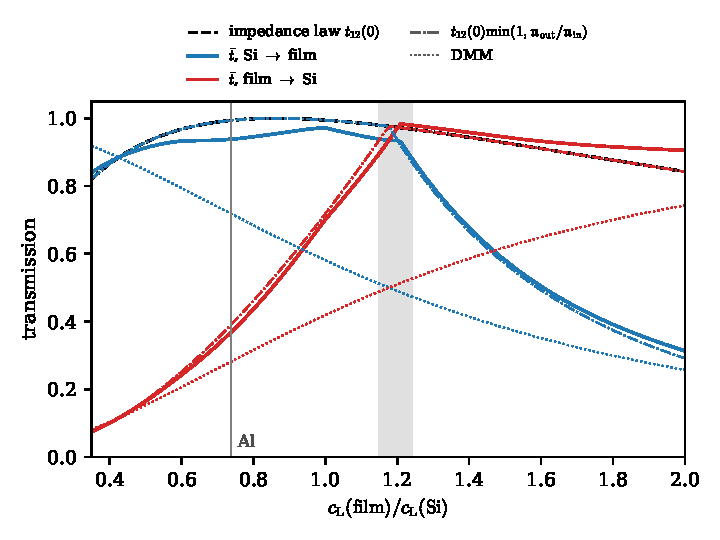
\includegraphics[width=\linewidth]{figures/ch20/limit20_3a.pdf}
\captionof{figure}{Transmission between isotropic silicon and a family of aluminum-like films against the ratio of their longitudinal speeds; the film keeps the density \SI{2.70}{g.cm^{-3}} and the aluminum ratio $c_{\mathrm{T}}/c_{\mathrm{LA}} = 0.498$, and $c_{\mathrm{LA}}(\mathrm{film})/c_{\mathrm{LA}}(\mathrm{Si}) = 0.737$ is aluminum (vertical line). Dashed: the impedance law. Solid: the averages \cref{eq:20.3-avg} from silicon into the film (blue) and back (red). Dash-dot: the leading correction, reciprocity \cref{eq:20.3-recip} applied to the impedance law on the slower side, $t_{12}(0)\min(1, \mathfrak{n}_{\mathrm{out}}/\mathfrak{n}_{\mathrm{in}})$, within \SI{6.9}{\percent} of the averages over the whole range. Dotted: the diffuse mismatch \cref{eq:20.3-dmm}. Gray: speed ratios 1.146 to 1.242, where the impedance law lies within \SI{10}{\percent} of the averages in both directions. In that range $\mathfrak{n}_{\mathrm{film}} \approx \mathfrak{n}_{\mathrm{Si}}$.}\label{fig:20-limit-amm}
\par}
\smallskip
Away from equal interface densities the critical angles of the slower medium's phonons, which the impedance law ignores, remove most of the flux in one direction: for aluminum on silicon the law overstates the escape from the film by a factor 2.70, while reciprocity applied to it, $t_{12}(0)\,\mathfrak{n}_{\mathrm{Si}}/\mathfrak{n}_{\mathrm{Al}} = 0.390$, comes within \SI{6}{\percent} of 0.368.
\end{limitbox}

\subsection{Film absorption and escape time}\label{sec:20.3-escape}

Inside a superconducting film a phonon of energy $E_{\mathrm{ath}}$ above $2\Delta_{\mathrm{BCS}}$ breaks a Cooper pair after a mean free path $\mathfrak{l}_{\mathrm{f}}(E_{\mathrm{ath}})$ (\cref{app:E.12}). Take a film of thickness $d_{\mathrm{f}}$ with a free top face and the substrate below. A phonon that moves at the angle $\theta$ to the normal travels $2d_{\mathrm{f}}/\cos\theta$ between two arrivals at the interface, where it escapes with probability $t_{\mathrm{esc}}$. If it keeps its angle, each round trip is survived with probability $\ee^{-y_{\mathrm{f}}/\cos\theta}$ and ends with an escape with probability $t_{\mathrm{esc}}$. Summing the geometric series of round trips, the probability that the phonon is absorbed before escaping is
\begin{equation}
  P_{\mathrm{abs}}(\theta) = \frac{1 - \ee^{-y_{\mathrm{f}}/\cos\theta}}{1 - (1 - t_{\mathrm{esc}})\,\ee^{-y_{\mathrm{f}}/\cos\theta}} ,
  \qquad y_{\mathrm{f}} = \frac{2d_{\mathrm{f}}}{\mathfrak{l}_{\mathrm{f}}} .
  \label{eq:20.3-pabs-theta}
\end{equation}
A polycrystalline film with a rough top face changes the direction of a phonon at every pass. Each round trip then starts from the flux distribution $2\sin\theta\cos\theta$ of \cref{eq:20.3-avg}, and with $\mu = \cos\theta$ the mean survival over one round trip is
\begin{equation*}
  \int_0^1 2\mu\,\ee^{-y_{\mathrm{f}}/\mu}\,\dd\mu = 2\int_1^\infty\frac{\ee^{-y_{\mathrm{f}}s}}{s^3}\,\dd s = 2E_3(y_{\mathrm{f}}) ,
\end{equation*}
with $s = 1/\mu$ and $E_3$ the exponential integral of order three. The escape probability becomes the average $\bar t_{\mathrm{esc}} = \bar t_{\mathrm{f\to sub}}$ of \cref{eq:20.3-avg}, and the absorption probability per entry is
\begin{equation}
  P_{\mathrm{abs}} = \frac{1 - 2E_3(y_{\mathrm{f}})}{1 - (1 - \bar t_{\mathrm{esc}})\,2E_3(y_{\mathrm{f}})} .
  \label{eq:20.3-pabs}
\end{equation}
For a thin film, $2E_3(y_{\mathrm{f}}) = 1 - 2y_{\mathrm{f}} + O(y_{\mathrm{f}}^2\ln y_{\mathrm{f}})$ and $P_{\mathrm{abs}} \simeq 4d_{\mathrm{f}}/(\mathfrak{l}_{\mathrm{f}}\bar t_{\mathrm{esc}})$: the phonon makes on average $1/\bar t_{\mathrm{esc}}$ round trips of mean length $4d_{\mathrm{f}}$ before it escapes.

The same counting in time gives the escape time. Let the film hold $N_\nu$ phonons of branch $\nu$ per unit volume, distributed isotropically. They strike unit area of the interface at the rate $N_\nu c_\nu/4$, of which the fraction $\langle t_\nu\rangle$, the angle integral in \cref{eq:20.3-avg}, escapes. The film holds $d_{\mathrm{f}}\sum_\nu N_\nu$ phonons per unit area. Let the branches be populated as in equilibrium at a fixed frequency, $N_\nu \propto c_\nu^{-3}$ by \cref{eq:5.2-dosac}. The escape rate is then
\begin{equation*}
  \frac{1}{t_l} = \frac{\sum_\nu N_\nu c_\nu\langle t_\nu\rangle}{4d_{\mathrm{f}}\sum_\nu N_\nu} = \frac{\mathfrak{n}_{\mathrm{f}}\,\bar t_{\mathrm{esc}}}{4d_{\mathrm{f}}\sum_\nu c_\nu^{-3}} .
\end{equation*}
\begin{keyresult}[Film escape time]
A phonon population that is isotropic and mixed among branches leaves a film of thickness $d_{\mathrm{f}}$ at the rate $1/t_l$, with
\begin{equation}
  t_l = \frac{4d_{\mathrm{f}}}{v_s\,\bar t_{\mathrm{esc}}} , \qquad v_s = \frac{\sum_\nu c_\nu^{-2}}{\sum_\nu c_\nu^{-3}} ,
  \label{eq:20.3-tl}
\end{equation}
where $v_s$ is the mean speed of the film's phonons weighted by their density of states and $\bar t_{\mathrm{esc}}$ the mean transmission into the substrate, \cref{eq:20.3-avg}.
\end{keyresult}
\Cref{eq:20.3-tl} assumes that the population is randomized in direction and branch faster than it escapes, that the transmissions are frequency independent, that the top face loses nothing, and that $\bar t_{\mathrm{esc}}$ is the transmission of a clean welded interface, or whatever replaces it. Without the mixing, the \SI{56}{\percent} of the flux beyond the transverse critical angle would never leave, and frequency independence needs wavelengths below $d_{\mathrm{f}}$. With the pair-breaking time $t_{\mathrm{pb}} = \mathfrak{l}_{\mathrm{f}}/v_s$, the thin-film limit of \cref{eq:20.3-pabs} reads $P_{\mathrm{abs}} \simeq t_l/t_{\mathrm{pb}}$, the first term of the competition $t_l/(t_l + t_{\mathrm{pb}})$ between escape and pair breaking.

\begin{workedexample}{Escape from a \SI{60}{nm} aluminum film on silicon}\label{we:20-escape}
The film phonons have $c_{\mathrm{LA}} = 6.63$ and $c_{\mathrm{T}} = \SI{3.30}{km.s^{-1}}$. The sums in \cref{eq:20.3-tl} are $\sum_\nu c_\nu^{-2} = \mathfrak{n}_{\mathrm{Al}} = \SI{0.2062}{s^2.km^{-2}}$ and $\sum_\nu c_\nu^{-3} = \SI{0.0590}{s^3.km^{-3}}$, so $v_s = \SI{3.50}{km.s^{-1}}$, close to the transverse speed because transverse modes dominate the density of states.

The escape probability is the average from aluminum into silicon. The acoustic mismatch model gives $\bar t_{\mathrm{esc}} = 0.368$, from 0.624 for longitudinal, 0.313 for SV and 0.359 for SH phonons; the diffuse mismatch model gives 0.282. With $d_{\mathrm{f}} = \SI{60}{nm}$,
\begin{equation*}
  t_l = \frac{4\times\SI{60}{nm}}{\SI{3.50}{km.s^{-1}}\times0.368} = \SI{0.187}{ns} \quad\text{(acoustic)}, \qquad \SI{0.244}{ns} \quad\text{(diffuse)},
\end{equation*}
a factor 1.31 between the two models. Near $2\Delta_{\mathrm{BCS}}$ a phonon in aluminum breaks a pair in the time $t_0 \approx \SI{0.26}{ns}$, the characteristic phonon lifetime of Kaplan and coworkers~\cite{kaplan1976quasiparticle}, \cite[p.~2]{guruswamy2014quasiparticle}, which \cref{sec:20.4} defines as the pair-breaking time at threshold. Hence $t_l/t_0 = 0.72$ (acoustic) or 0.94 (diffuse). A \SI{60}{nm} film loses its phonons about as fast as they break pairs, which is the regime in which \cref{sec:20.4} finds the quasiparticle yield sensitive to $t_l/t_0$. If the mean free path were $\mathfrak{l}_{\mathrm{f}} = v_st_0 = \SI{0.909}{\micro m}$, then $y_{\mathrm{f}} = 0.132$ and \cref{eq:20.3-pabs} would give $P_{\mathrm{abs}} = 0.422$, against $t_l/(t_l + t_0) = 0.418$.
\end{workedexample}

\subsection{The fitted silicon-to-aluminum coefficient}\label{sec:20.3-fit}

Martinez and coworkers illuminated the back of silicon wafers 300 to \SI{380}{\micro m} thick, \SI{2}{cm} square, that carried \SI{60}{nm} aluminum resonators. They compared the measured phonon pulses with a Monte Carlo simulation using specular reflection, and the silicon-to-aluminum coefficient that reproduced the data lay between 0.30 and 0.55~\cite[Sect.~V]{martinez2019measurements}. Their simulation does not propagate phonons inside the aluminum. A phonon that crosses produces a signal with the pair-breaking efficiency or is removed, and the fitted coefficient's complement includes phonons that enter the film and come back~\cite[Sect.~IV]{martinez2019measurements}. The fitted coefficient is therefore the probability that a phonon arriving from silicon is absorbed in the film,
\begin{equation}
  T_{\mathrm{fit}} = \bar t_{\mathrm{Si\to Al}}\,P_{\mathrm{abs}} .
  \label{eq:20.3-Tfit}
\end{equation}
With the acoustic-mismatch value 0.938, the fit gives $P_{\mathrm{abs}} = 0.320$ to 0.586. Inverting \cref{eq:20.3-pabs} with $\bar t_{\mathrm{esc}} = 0.368$ gives $\mathfrak{l}_{\mathrm{f}}/d_{\mathrm{f}} = 23.1$ to 8.3, or $\mathfrak{l}_{\mathrm{f}} = 1.39$ to \SI{0.50}{\micro m}, and $t_{\mathrm{pb}} = \mathfrak{l}_{\mathrm{f}}/v_s = 0.40$ to \SI{0.14}{ns}, the same order as $t_0$. Keeping the angle of each phonon instead, \cref{eq:20.3-pabs-theta} averaged with $t_{\mathrm{esc}} = \bar t_{\mathrm{esc}}$ gives 1.29 to \SI{0.46}{\micro m}; the diffuse-mismatch pair, 0.718 and 0.282, gives 1.19 to \SI{0.31}{\micro m}. The fit thus constrains the pair-breaking length over the thickness, $\mathfrak{l}_{\mathrm{f}}/d_{\mathrm{f}} \approx 5$ to 23 across both models, and says little about the interface. In the thin-film limit $T_{\mathrm{fit}} \to (\mathfrak{n}_{\mathrm{Al}}/\mathfrak{n}_{\mathrm{Si}})\,4d_{\mathrm{f}}/\mathfrak{l}_{\mathrm{f}}$ for any interface that conserves energy, by reciprocity (\cref{eq:20.3-pabs,eq:20.3-recip}), and the interface model enters only through the finite-thickness corrections. Read as a transmission, the fit would put the escape probability at $(\mathfrak{n}_{\mathrm{Si}}/\mathfrak{n}_{\mathrm{Al}})\times(0.30$ to $0.55) = 0.118$ to 0.216 by \cref{eq:20.3-recip}, below both models. The inferred lengths are estimates: they inherit the specular, mode-conserving simulation of the fit and the isotropic averages of this section. An earlier silicon detector model matched its data with a \SI{33}{\percent} probability for a phonon to be absorbed at an amorphous-silicon/aluminum interface, the rest scattering back diffusely~\cite[Sect.~III\,G]{leman2012invited}; that coefficient is an absorption probability of the same kind.

\subsection{Anisotropy and interlayers}\label{sec:20.3-aniso}

The isotropic averages hide the anisotropy of silicon, whose longitudinal speed ranges from 8.43 to \SI{9.35}{km.s^{-1}} and whose transverse speeds from 4.67 to \SI{5.84}{km.s^{-1}} (\cref{eq:C.18-cubic}). Giving the isotropic silicon its $[100]$ speeds, 8.43 and \SI{5.84}{km.s^{-1}}, or its $[111]$ speeds, 9.35 and \SI{5.09}{km.s^{-1}}, moves $\bar t_{\mathrm{esc}}$ from 0.368 to 0.327 and 0.405, and $t_l$ for \SI{60}{nm} from 0.187 to 0.210 and \SI{0.169}{ns}; $\bar t_{\mathrm{Si\to Al}}$ moves only between 0.927 and 0.943. These are sensitivities, not bounds. The texture of the film matters less, since it changes the longitudinal speed of aluminum by at most \SI{3}{\percent} (\cref{app:C.18}). In the anisotropic problem the critical angles depend on the direction in the interface plane, the group velocity is not parallel to $\vect{Q}$, and the plane waves on each side follow from the Christoffel equation \cref{eq:C.18-christoffel}; the boundary problem becomes six by six. The reciprocity \cref{eq:20.3-recip} holds there unchanged.

Real interfaces carry a native oxide or a deposited amorphous layer a few nanometers thick. A flat layer that does not dissipate cannot change which waves propagate in silicon, since $Q_\parallel$ is conserved through every layer: the critical angles and the \SI{56}{\percent} of trapped film flux stay as they are. The layer changes the transmission inside the cone. At normal incidence take a layer of impedance $Z_{\mathrm{ac},3}$, speed $c_3$ and thickness $h$. At the quarter-wave frequency $c_3/4h$ the wave crosses it with the phase $\pi/2$, and the layer maps the particle velocity $\dot u$ and the force $-\sigma_{zz}$ at its far face onto $\ii(-\sigma_{zz})/Z_{\mathrm{ac},3}$ and $\ii Z_{\mathrm{ac},3}\dot u$ at its near face. A medium of impedance $Z_{\mathrm{ac},2}$ behind it then looks like one of impedance $Z_{\mathrm{ac},3}^2/Z_{\mathrm{ac},2}$, and \cref{eq:C.18-transmission} with this replacement gives the lowest transmission,
\begin{equation*}
  t_{\min} = \frac{4Z_{\mathrm{ac},1}Z_{\mathrm{ac},2}Z_{\mathrm{ac},3}^2}{\bigl(Z_{\mathrm{ac},1}Z_{\mathrm{ac},2} + Z_{\mathrm{ac},3}^2\bigr)^2} ,
\end{equation*}
since the transmission oscillates between this value and the bare $t_{12}(0)$ as the frequency varies. Amorphous SiO$_2$, with $\rho_T = \SI{2.2}{g.cm^{-3}}$ and $\rho_Tc_{\mathrm{LA}}^2 = \SI{7.40e10}{Pa}$ (\cref{sec:16.7}), has $c_{\mathrm{LA}} = \SI{5.80}{km.s^{-1}}$ and $Z_{\mathrm{ac}} = \SI{12.8e6}{kg.m^{-2}.s^{-1}}$. Between silicon and aluminum it gives $t_{\min} = 0.844$, against 0.994 without the layer, at \SI{0.72}{THz} for a \SI{2}{nm} layer; a \SI{1}{nm} layer transmits 0.901 at \SI{0.8}{THz}. A rough or disordered layer scatters diffusely instead, does not conserve $Q_\parallel$, and can release trapped modes; the diffuse mismatch model is the limit of complete randomization. Until the escape probability of a real film is measured, the spread from 0.282 to 0.368, a factor 1.31 in $t_l$, is the uncertainty to carry.

\section{Quasiparticle yield in superconductors}\label{sec:20.4}

A phonon of \SI{0.59}{THz}, at the soft end of what a silicon crystal delivers to its sensors after down-conversion (\cref{sec:20.5-meanfield}), carries \SI{2.45}{meV} into an aluminum film, 13.6 times the gap $\Delta_{\mathrm{BCS}} = \SI{0.18}{meV}$ of \cref{sec:7.2}. The sensor counts quasiparticles, and each of them, once it has relaxed to the gap edge, holds $\Delta_{\mathrm{BCS}}$. Were all of the phonon's energy spent on breaking pairs, it would make 13.6 quasiparticles. In a film thick enough to keep every phonon it makes about eight, and in a thin film on a substrate fewer than five. The fraction of the phonon energy that ends up in quasiparticles, the quasiparticle or pair-breaking efficiency $Y_{\mathrm{qp}}$, multiplies every phonon collection efficiency $\epsilon$ of \cref{sec:19.5}, and it depends on the phonon energy. We will derive it exactly below four gaps and write the cascade of phonons and quasiparticles that sets it above. Above four gaps it falls with the time $t_l$ that a phonon spends in the film before escaping, which \cref{sec:20.3} relates to the film thickness and the interface.

\subsection{Pair breaking below four gaps}\label{sec:20.4-below}

Let a phonon of energy $E_{\mathrm{ath}} \ge 2\Delta_{\mathrm{BCS}}$ break a pair in a film at a temperature far below $T_c$, where thermal quasiparticles are absent (\cref{eq:7.2-threshold}). Within 0.1 to \SI{10}{ns}~\cite[p.~1]{guruswamy2014quasiparticle} every quasiparticle it has produced has relaxed to the gap edge, and the rest of its energy has left as phonons that can no longer break pairs. If $N_{\mathrm{qp}}$ quasiparticles are left, the yield of the event is
\begin{equation}
  Y_{\mathrm{qp}}(E_{\mathrm{ath}}) \equiv \frac{\Delta_{\mathrm{BCS}}\langle N_{\mathrm{qp}}\rangle}{E_{\mathrm{ath}}}
  = 1 - \frac{\langle E_{\mathrm{sub}} + E_{\mathrm{leak}}\rangle}{E_{\mathrm{ath}}} ,
  \label{eq:20.4-Y}
\end{equation}
where $E_{\mathrm{sub}}$ is the energy carried off by phonons below $2\Delta_{\mathrm{BCS}}$ and $E_{\mathrm{leak}}$ that of phonons above $2\Delta_{\mathrm{BCS}}$ that leave the film before they break a pair. The second form is the energy balance $E_{\mathrm{ath}} = \Delta_{\mathrm{BCS}}N_{\mathrm{qp}} + E_{\mathrm{sub}} + E_{\mathrm{leak}}$, event by event. We count the yield for a phonon that has broken its first pair. Whether an arriving phonon is absorbed at all is the absorption probability of \cref{sec:20.3}, and a sensor efficiency is the product of the two.

The split of the pair energy, the pair-breaking rate and the emission rate of a hot quasiparticle all follow from the golden rule with the coherence factors of \cref{eq:7.2-cohE}. The phonon couples to the electron density, so its absorption is case~I. Its momentum is $E_{\mathrm{ath}}$ divided by the sound speed. Since the longitudinal sound speed of aluminum, \SI{6.63}{km/s} (\cref{sec:20.3}), is 305 times below $v_{\mathrm{F}} = \num{6.75e-3}$, or \SI{2.0e6}{m/s} (\cref{sec:7.2}), the condition $v_{\mathrm{F}}q \ge E_{\mathrm{ath}}$ of \cref{eq:7.2-pairspec} holds with a wide margin. The energies $\xi$ and $\xi'$ of the two electrons are then independent, the terms odd in them average out, and the creation factor is $\frac12(1 + \Delta_{\mathrm{BCS}}^2/EE')$. Each final quasiparticle is weighted with its density of states \cref{eq:7.2-dos}. The probability that one of the two receives the energy $E$, and the other $E_{\mathrm{ath}} - E$, is then
\begin{equation}
  P_{\mathrm{pb}}(E\,|\,E_{\mathrm{ath}}) = \frac{1}{E_{\mathrm{ath}}\mathfrak{g}_{\mathrm{I}}(E_{\mathrm{ath}}/\Delta_{\mathrm{BCS}})}\,
  \frac{E(E_{\mathrm{ath}} - E) + \Delta_{\mathrm{BCS}}^2}{\sqrt{E^2 - \Delta_{\mathrm{BCS}}^2}\,\sqrt{(E_{\mathrm{ath}} - E)^2 - \Delta_{\mathrm{BCS}}^2}} ,
  \label{eq:20.4-split}
\end{equation}
for $\Delta_{\mathrm{BCS}} \le E \le E_{\mathrm{ath}} - \Delta_{\mathrm{BCS}}$. The normalization is the case-I ratio $\mathfrak{g}_{\mathrm{I}} = S_{\mathrm{I}}/S_{\mathrm{n}}$ of \cref{eq:7.2-pairspec,eq:15.1-gI}: the integral of the numerator over the denominator is $E_{\mathrm{ath}}\mathfrak{g}_{\mathrm{I}}$. The split is symmetric about $E_{\mathrm{ath}}/2$ and peaked at both ends, where the density of states diverges. A photon couples through the current, which is case~II, and its split has $-\Delta_{\mathrm{BCS}}^2$ in the numerator~\cite[Eq.~(1)]{guruswamy2014quasiparticle}.

The same ratio fixes how fast the phonon breaks a pair. In the normal metal a phonon decays into an electron--hole pair at the rate given by Allen's formula \cref{eq:6.4-allen}. The superconductor changes only the phase space of the pair and its coherence factor, which together multiply the normal rate by $\mathfrak{g}_{\mathrm{I}}$. At low energies the Eliashberg function of a metal grows as $\alpha^2F = b_\alpha E_{\mathrm{ath}}^2$, the form behind the factor quadratic in the phonon energy in the spectrum of emitted phonons given by Leman~\cite[Sect.~IV]{leman2012invited}. With a phonon density of states $\propto E_{\mathrm{ath}}^2$, this $\alpha^2F$ gives a normal-state width linear in $E_{\mathrm{ath}}$ (\cref{eq:6.4-lambda}). Measuring the pair-breaking time $t_{\mathrm{pb}}$ in units of its value $t_0$ at threshold, where $\mathfrak{g}_{\mathrm{I}} = \pi/2$, we find
\begin{equation}
  \frac{1}{t_{\mathrm{pb}}(E_{\mathrm{ath}})} = \frac{E_{\mathrm{ath}}\,\mathfrak{g}_{\mathrm{I}}(E_{\mathrm{ath}}/\Delta_{\mathrm{BCS}})}{\pi\Delta_{\mathrm{BCS}}\,t_0} ,
  \label{eq:20.4-tpb}
\end{equation}
the zero-temperature pair-breaking rate. Since $\mathfrak{g}_{\mathrm{I}}$ falls from $\pi/2$ to one, the rate rises linearly with energy at large $E_{\mathrm{ath}}$, the approximate scaling $t_{\mathrm{pb}} \propto 1/E_{\mathrm{ath}}$ of Kaplan et al.~\cite{kaplan1976quasiparticle} as quoted by Guruswamy et al.~\cite[p.~5]{guruswamy2014quasiparticle}, and a phonon of $10\Delta_{\mathrm{BCS}}$ breaks a pair in $0.30\,t_0$. For aluminum, Guruswamy et al.\ take $t_0 = \SI{0.26}{ns}$~\cite[p.~3]{guruswamy2014quasiparticle}. The conserving correction of \cref{sec:7.2} plays no role here: it is controlled by $\Delta_{\mathrm{BCS}}/v_{\mathrm{F}}q$, at most \num{1.6e-3} for a phonon above the threshold.

A quasiparticle of energy $E$ relaxes by emitting a phonon of energy $E_{\mathrm{ath}}$ and dropping to $E - E_{\mathrm{ath}}$. This is quasiparticle scattering, with the case-I factor $\frac12(1 - \Delta_{\mathrm{BCS}}^2/EE')$ after the same average, and the rate per unit phonon energy is
\begin{equation}
  \varGamma_{\mathrm{qp,em}}(E_{\mathrm{ath}}\,|\,E) \propto \alpha^2F(E_{\mathrm{ath}})\,\frac{E - E_{\mathrm{ath}}}{\sqrt{(E - E_{\mathrm{ath}})^2 - \Delta_{\mathrm{BCS}}^2}}\Bigl[1 - \frac{\Delta_{\mathrm{BCS}}^2}{E(E - E_{\mathrm{ath}})}\Bigr] ,
  \label{eq:20.4-emit}
\end{equation}
for $0 \le E_{\mathrm{ath}} \le E - \Delta_{\mathrm{BCS}}$, again a rate first given by Kaplan et al.~\cite{kaplan1976quasiparticle}; with $\alpha^2F \propto E_{\mathrm{ath}}^2$ it is the phonon distribution quoted by Leman~\cite[Sect.~IV]{leman2012invited}. The middle factor is the density of final quasiparticle states, \cref{eq:7.2-dos} over its normal value. The overall scale, set by the electron--phonon coupling and expressed as a characteristic time of \SI{438}{ns} for aluminum~\cite[p.~3]{guruswamy2014quasiparticle}, does not affect the yield, because a quasiparticle stays in the film whatever time it takes to relax. At zero temperature it can only lose energy, and it does so until it reaches the gap edge.

\begin{keyresult}[Pair-breaking efficiency below four gaps]
A phonon of energy $E_{\mathrm{ath}}$ that breaks a pair in a superconductor at $T \ll T_c$ leaves exactly two quasiparticles if $E_{\mathrm{ath}} < 4\Delta_{\mathrm{BCS}}$, and
\begin{equation}
  Y_{\mathrm{qp}}(E_{\mathrm{ath}}) = \frac{2\Delta_{\mathrm{BCS}}}{E_{\mathrm{ath}}} , \qquad 2\Delta_{\mathrm{BCS}} \le E_{\mathrm{ath}} < 4\Delta_{\mathrm{BCS}} ,
  \label{eq:20.4-below}
\end{equation}
whatever the film thickness, the shape of $\alpha^2F$ and the split \cref{eq:20.4-split}.
\end{keyresult}
\noindent The proof is kinematic. A quasiparticle at $E$ can emit a phonon that breaks a further pair only if the phonon has at least $2\Delta_{\mathrm{BCS}}$ and the quasiparticle is left with at least $\Delta_{\mathrm{BCS}}$, that is, only if $E \ge 3\Delta_{\mathrm{BCS}}$. The hotter of the two quasiparticles from the first pair has at most $E_{\mathrm{ath}} - \Delta_{\mathrm{BCS}}$, since its partner has at least $\Delta_{\mathrm{BCS}}$. A third quasiparticle therefore requires $E_{\mathrm{ath}} \ge 4\Delta_{\mathrm{BCS}}$. Below that energy each quasiparticle relaxes by emitting phonons of less than $2\Delta_{\mathrm{BCS}}$, which cannot break pairs, and $E_{\mathrm{ath}} - 2\Delta_{\mathrm{BCS}}$ leaves as $E_{\mathrm{sub}}$, while $E_{\mathrm{leak}} = 0$. Escape cannot compete, because no phonon of the event other than the first is able to break a pair. Guruswamy et al.\ find the same result in the kinetic equations, a yield that ``reduces monotonically and is independent of the phonon loss time'' between two and four gaps~\cite[p.~5]{guruswamy2014quasiparticle}. The argument uses only the threshold \cref{eq:7.2-threshold} and the loss of energy by quasiparticles, so it holds for a photon and for a dark-matter particle that deposits $\omega$ in an aluminum target (\cref{sec:15.1}) as well. Each phonon and each photon of the band from $2\Delta_{\mathrm{BCS}}$ to $4\Delta_{\mathrm{BCS}}$, 87 to \SI{174}{GHz} in aluminum, makes exactly two quasiparticles, and a sensor that counts them has no fluctuation from the film at all.

\begin{workedexample}{The yield of a $3\Delta_{\mathrm{BCS}}$ phonon in aluminum}\label{we:20-al3}
With $\Delta_{\mathrm{BCS}} = \SI{0.18}{meV}$ a phonon of $3\Delta_{\mathrm{BCS}}$ has \SI{0.54}{meV}, or \SI{131}{GHz}. It lies above the pair-breaking threshold $2\Delta_{\mathrm{BCS}} = \SI{0.36}{meV}$ (\SI{87.0}{GHz}). From \cref{eq:20.4-tpb} with $\mathfrak{g}_{\mathrm{I}}(3) = 1.322$ (\cref{sec:15.1}), it breaks a pair after $t_{\mathrm{pb}} = \pi t_0/(3 \times 1.322) = 0.792\,t_0 = \SI{0.206}{ns}$ on average, with $t_0 = \SI{0.26}{ns}$. By \cref{eq:20.4-split} one quasiparticle receives an energy $E$ between $\Delta_{\mathrm{BCS}}$ and $2\Delta_{\mathrm{BCS}}$ and the other $3\Delta_{\mathrm{BCS}} - E$, with both ends of that interval favored. The hotter one has at most $2\Delta_{\mathrm{BCS}}$, less than the $3\Delta_{\mathrm{BCS}}$ it would need to emit a pair-breaking phonon. Each quasiparticle relaxes by \cref{eq:20.4-emit}, emitting phonons of at most $E - \Delta_{\mathrm{BCS}} \le \Delta_{\mathrm{BCS}}$, that is below \SI{43.5}{GHz}. The event ends with $N_{\mathrm{qp}} = 2$ every time, and
\begin{equation*}
  Y_{\mathrm{qp}}(3\Delta_{\mathrm{BCS}}) = \frac{2}{3} , \qquad E_{\mathrm{sub}} = \Delta_{\mathrm{BCS}} = \SI{0.18}{meV} , \qquad E_{\mathrm{leak}} = 0 .
\end{equation*}
The film thickness enters only through the chance that the phonon is absorbed before it escapes, the absorption probability of \cref{sec:20.3}. Once it is absorbed, a film of \SI{30}{nm} and one of \SI{1}{\micro m} give the same two quasiparticles. The \SI{2.45}{meV} phonon of the opening, at $13.6\,\Delta_{\mathrm{BCS}}$, already has a yield between 0.31 and 0.59 depending on the film (\cref{sec:20.4-film}).
\end{workedexample}

\subsection{The Kaplan cascade}\label{sec:20.4-cascade}

Above $4\Delta_{\mathrm{BCS}}$ the hot quasiparticles emit phonons that break further pairs, those pairs yield further hot quasiparticles, and the energy comes down in generations, with phonons and quasiparticles alternating. Detector physicists call this the Kaplan cascade, after the rates of Kaplan et al.~\cite{kaplan1976quasiparticle}. Every phonon above $2\Delta_{\mathrm{BCS}}$ now either breaks a pair after $t_{\mathrm{pb}}$ or leaves the film after the escape time $t_l = 4d_{\mathrm{f}}/(v_s\bar t_{\mathrm{esc}})$ of \cref{sec:20.3}. In the lumped-film model the film is one object: it holds a phonon for an exponentially distributed time of mean $t_l$, whatever the phonon's energy and position~\cite[p.~2]{guruswamy2014quasiparticle}. The two processes compete as independent decays, and a phonon breaks a pair with the probability
\begin{equation}
  p_{\mathrm{pb}}(E_{\mathrm{ath}}) = \frac{1}{1 + t_{\mathrm{pb}}(E_{\mathrm{ath}})/t_l}
  = \frac{E_{\mathrm{ath}}\mathfrak{g}_{\mathrm{I}}}{E_{\mathrm{ath}}\mathfrak{g}_{\mathrm{I}} + \pi\Delta_{\mathrm{BCS}}\,t_0/t_l} .
  \label{eq:20.4-ppb}
\end{equation}
Hard phonons break pairs before they escape, since $t_{\mathrm{pb}}$ falls as $1/E_{\mathrm{ath}}$. The losses, however, concentrate on the phonons a few gaps above threshold, and every cascade passes through them.

In the lumped film a quasiparticle never leaves, so the only times that compete are $t_{\mathrm{pb}}$ and $t_l$, and the yield depends on the film through $t_l/t_0$ alone. Since the quasiparticles are dilute during the cascade and the temperature is far below $T_c$, every particle develops independently of the others. The cascade is then a branching process of the kind treated in \cref{sec:18.1}, and its mean obeys linear equations. Let $\bar N_{\mathrm{qp}}(E)$ be the mean number of quasiparticles that end at the gap edge from one quasiparticle of energy $E$, itself included, and $\bar N_{\mathrm{ph}}(E_{\mathrm{ath}})$ the same number for one phonon. Averaging over the first step of each,
\begin{equation}
  \begin{aligned}
  \bar N_{\mathrm{qp}}(E) &= \int_0^{E - \Delta_{\mathrm{BCS}}}\dd E_{\mathrm{ath}}\,w(E_{\mathrm{ath}}\,|\,E)\,\bigl[\bar N_{\mathrm{qp}}(E - E_{\mathrm{ath}}) + \bar N_{\mathrm{ph}}(E_{\mathrm{ath}})\bigr] ,\\
  \bar N_{\mathrm{ph}}(E_{\mathrm{ath}}) &= p_{\mathrm{pb}}(E_{\mathrm{ath}})\int\dd E\,P_{\mathrm{pb}}(E\,|\,E_{\mathrm{ath}})\,\bigl[\bar N_{\mathrm{qp}}(E) + \bar N_{\mathrm{qp}}(E_{\mathrm{ath}} - E)\bigr]
  \end{aligned} ,
  \label{eq:20.4-cascade}
\end{equation}
the first for $E \ge 3\Delta_{\mathrm{BCS}}$ and the second for $E_{\mathrm{ath}} \ge 2\Delta_{\mathrm{BCS}}$, with $\bar N_{\mathrm{qp}} = 1$ below $3\Delta_{\mathrm{BCS}}$ and $\bar N_{\mathrm{ph}} = 0$ below $2\Delta_{\mathrm{BCS}}$. Here $w = \varGamma_{\mathrm{qp,em}}/\int\varGamma_{\mathrm{qp,em}}$ is the normalized spectrum of the emitted phonon from \cref{eq:20.4-emit}. The yield of a phonon that has broken its first pair is $Y_{\mathrm{qp}} = \Delta_{\mathrm{BCS}}\bar N_{\mathrm{ph}}(E_{\mathrm{ath}})/[p_{\mathrm{pb}}(E_{\mathrm{ath}})E_{\mathrm{ath}}]$. The equations close on themselves from below: $\bar N_{\mathrm{ph}}$ at $E_{\mathrm{ath}}$ needs $\bar N_{\mathrm{qp}}$ only up to $E_{\mathrm{ath}} - \Delta_{\mathrm{BCS}}$, and $\bar N_{\mathrm{qp}}$ at $E$ needs $\bar N_{\mathrm{ph}}$ up to $E - \Delta_{\mathrm{BCS}}$. Below $4\Delta_{\mathrm{BCS}}$ they return \cref{eq:20.4-below} at once, since $\bar N_{\mathrm{qp}} = 1$ for both quasiparticles of the first pair. The only material inputs are the shape of $\alpha^2F$ below $E_{\mathrm{ath}}$ and the ratio $t_l/t_0$; the coupling strength $b_\alpha$ cancels.

We solve \cref{eq:20.4-cascade} on an energy grid of step $0.01\Delta_{\mathrm{BCS}}$ with $\alpha^2F = b_\alpha E_{\mathrm{ath}}^2$. Substituting $E = \Delta_{\mathrm{BCS}} + (E_{\mathrm{ath}} - 2\Delta_{\mathrm{BCS}})\sin^2\theta$ in the split, and a quadratic map onto the edge in the emission integral, removes the inverse-square-root edges of the densities of states, and we iterate from $\bar N_{\mathrm{qp}} = 1$ to convergence. An event-by-event simulation with the same kernels agrees with the solution within 1.2 standard errors, about 0.001. The low-frequency form of $\alpha^2F$ restricts the result to phonon energies well below the transverse peak of the aluminum Eliashberg function at \SI{23}{meV} (\cref{sec:6.4}), and we stop at $60\Delta_{\mathrm{BCS}} = \SI{10.8}{meV}$. In practice the cascade is run inside detector simulations (\cref{app:E.12}).

In the limit $t_l \to \infty$ nothing escapes. The yield then rises from 0.5 at $4\Delta_{\mathrm{BCS}}$ to a maximum of 0.600 at $5.46\,\Delta_{\mathrm{BCS}}$ and settles at 0.590, between 0.5901 and 0.5905 over the whole range from 10 to $60\Delta_{\mathrm{BCS}}$. This is the infinite-volume value that earlier calculations found for aluminum, niobium and tin, 0.57 to 0.6~\cite[p.~2]{guruswamy2014quasiparticle}. About \SI{41}{\percent} of a hard phonon's energy is therefore lost even without escape. The loss goes into the sub-gap phonons that every quasiparticle emits on its last steps to the edge, and into the quasiparticles that end between $\Delta_{\mathrm{BCS}}$ and $3\Delta_{\mathrm{BCS}}$ and have to shed their excess without breaking a pair. The asymptote is independent of energy because the cascade is self-similar while $E \gg \Delta_{\mathrm{BCS}}$. A quasiparticle far above the gap emits phonons with the spectrum $E_{\mathrm{ath}}^2$ on $[0, E]$, which has the mean $3E/4$, and every generation passes energy down in the same proportions until the last few generations near the gap, which set the loss. The split \cref{eq:20.4-split} of the first pair matters only near threshold. Without escape, a phonon seed and a photon seed differ by 0.007 at $5\Delta_{\mathrm{BCS}}$ and by less than 0.001 at $10\Delta_{\mathrm{BCS}}$.

\subsection{Thin films and the Chang--Scalapino equations}\label{sec:20.4-film}

In a film the ratio $t_l/t_0$ decides how much more is lost. \Cref{fig:20-yield}(a) shows the yield from \cref{eq:20.4-cascade} for $t_l/t_0$ from 0.5 to 8 and in the infinite-volume limit. For $t_l/t_0 = 4$, a phonon breaks a pair before it escapes with the probability \cref{eq:20.4-ppb} of 0.84 at $3\Delta_{\mathrm{BCS}}$ and 0.93 at $10\Delta_{\mathrm{BCS}}$, and these losses compound over the generations. Above $4\Delta_{\mathrm{BCS}}$ the yield first rises a little, to 0.560 at $5.2\,\Delta_{\mathrm{BCS}}$ for $t_l/t_0 = 4$, and then falls: at $10\Delta_{\mathrm{BCS}}$ it is 0.349, 0.415, 0.477, 0.524 and 0.554 for $t_l/t_0 = 0.5$, 1, 2, 4 and 8, against 0.590 without escape. For $t_l/t_0 = 0.5$ the rise has disappeared, and the yield falls from the start, to 0.238 at $60\Delta_{\mathrm{BCS}}$. The \SI{60}{nm} film of \cref{we:20-escape}, at $t_l/t_0 = 0.72$ to 0.94, has 0.383 to 0.409 at $10\Delta_{\mathrm{BCS}}$. Two effects compete above four gaps. A hotter phonon can make more pairs, which raises the yield, but its energy passes through more generations of phonons, each of which can escape. The second effect wins at all energies above about $5\Delta_{\mathrm{BCS}}$ for every finite $t_l$.

\begin{figure}[tbp]
  \centering
  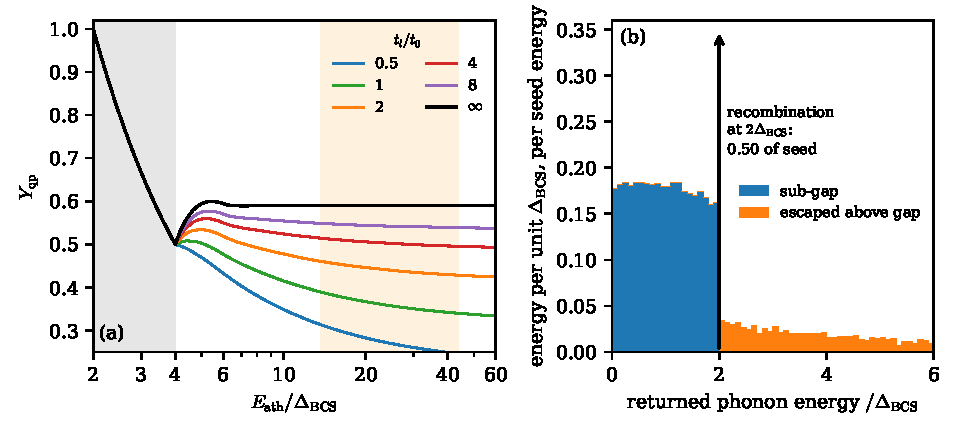
\includegraphics[width=\linewidth]{figures/ch20/fig20_4.pdf}
  \caption{Quasiparticle yield of an aluminum film from the Kaplan cascade in a lumped film at zero temperature, \cref{eq:20.4-cascade}, with $\alpha^2F \propto E_{\mathrm{ath}}^2$ and the pair-breaking time \cref{eq:20.4-tpb}. (a) Yield $Y_{\mathrm{qp}} = \Delta_{\mathrm{BCS}}\langle N_{\mathrm{qp}}\rangle/E_{\mathrm{ath}}$ of a phonon that has broken its first pair, against its energy in units of the gap, for six ratios of the film escape time to the pair-breaking time at threshold, $t_l/t_0$. Gray: below $4\Delta_{\mathrm{BCS}}$, where $Y_{\mathrm{qp}} = 2\Delta_{\mathrm{BCS}}/E_{\mathrm{ath}}$ exactly for every film. Tan: 2.45 to \SI{7.88}{meV}, or 13.6 to $43.8\,\Delta_{\mathrm{BCS}}$ at $\Delta_{\mathrm{BCS}} = \SI{0.18}{meV}$ (0.59 to \SI{1.91}{THz}), the band that holds the middle \SI{80}{\percent} of the primary-phonon energy absorbed in the mean-field silicon detector of \cref{sec:20.5-meanfield}. (b) Energy spectrum of the phonons that a thick film ($t_l/t_0 = 4$) returns to the substrate when a phonon of $40\Delta_{\mathrm{BCS}}$ cascades in it, per unit energy and per unit seed energy (event simulation, 4000 events). Blue: sub-gap relaxation phonons; orange: phonons above $2\Delta_{\mathrm{BCS}}$ that escape before breaking a pair. Arrow: the share 0.50 held by quasiparticles, which comes back later as recombination phonons of $2\Delta_{\mathrm{BCS}}$.}
  \label{fig:20-yield}
\end{figure}

Kinetic equations follow the same physics with fewer approximations. Chang and Scalapino wrote coupled Boltzmann equations for the quasiparticle distribution $f(E)$ and the phonon distribution $n(E_{\mathrm{ath}})$ of a superconductor, with the full energy dependence of the rates at finite temperature and the recombination of quasiparticles into $2\Delta_{\mathrm{BCS}}$ phonons~\cite{chang1977kinetic,chang1978nonequilibrium}. Guruswamy et al.\ solved them in steady state, with the phonon loss time $t_l$, for an aluminum film driven by photons of 2 to $10\Delta_{\mathrm{BCS}}$. They used the measured Eliashberg function, $T/T_c = 0.1$ and a weak microwave probe of the kind that reads out a resonator~\cite[Fig.~4]{guruswamy2014quasiparticle}. The cascade \cref{eq:20.4-cascade} is their equations linearized about the empty superconductor at zero temperature, with $\alpha^2F$ replaced by its low-frequency form, and the difference between the two measures what the linearization and the low-frequency $\alpha^2F$ leave out. \Cref{lim:20.4a} compares them for a photon seed, so that like is compared with like. For $t_l/t_0 \le 4$ the kinetic equations lie above the cascade by 0.001 to 0.011 at every energy from 5 to $10\Delta_{\mathrm{BCS}}$. For $t_l/t_0 = 8$ the offset is 0.036 to 0.041, nearly constant in energy, and the kinetic equations return 0.59 to 0.61 there, close to the infinite-volume value. The probe itself raises the yield by about \SI{2}{\percent}~\cite[Sect.~V]{guruswamy2014quasiparticle}. Counting the excess energy of the quasiparticles above the gap, rather than $\Delta_{\mathrm{BCS}}$ for each, would raise it by about \SI{4}{\percent}~\cite[Sect.~V]{guruswamy2014quasiparticle}; \cref{eq:20.4-Y} uses the gap-edge count, as they do.

\begin{limitbox}[Pair-breaking efficiency][lim:20.4a]
A pair-breaking quantum of energy $E_{\mathrm{ath}}$ between $2\Delta_{\mathrm{BCS}}$ and $4\Delta_{\mathrm{BCS}}$ yields $Y_{\mathrm{qp}} = 2\Delta_{\mathrm{BCS}}/E_{\mathrm{ath}}$, independent of the film; the infinite-volume yield at high energy is 0.57 to 0.6~\cite[pp.~2, 5]{guruswamy2014quasiparticle}.
\par\smallskip
{\centering
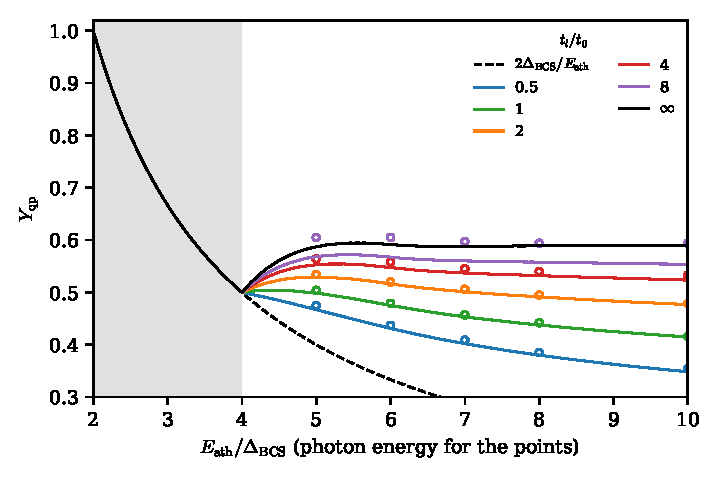
\includegraphics[width=\linewidth]{figures/ch20/limit20_4a.pdf}
\captionof{figure}{Yield of an aluminum film against the energy of the pair-breaking quantum in units of the gap. Dashed: $2\Delta_{\mathrm{BCS}}/E_{\mathrm{ath}}$, \cref{eq:20.4-below}. Lines: the Kaplan cascade \cref{eq:20.4-cascade} in a lumped film at zero temperature with $\alpha^2F \propto E_{\mathrm{ath}}^2$, for a photon seed (case-II split), at the ratios $t_l/t_0$ of the escape time to the pair-breaking time at threshold given in the legend. Circles: the coupled kinetic equations of Chang and Scalapino with the measured $\alpha^2F$ of aluminum at $T/T_c = 0.1$ with a microwave probe, read off~\cite[Fig.~4]{guruswamy2014quasiparticle} at the same $t_l/t_0$ (colors; digitized to $\pm0.005$). Gray: $E_{\mathrm{ath}} < 4\Delta_{\mathrm{BCS}}$, where the formula is exact. For $t_l/t_0 \le 4$ the cascade lies below the circles by at most 0.011; for $t_l/t_0 = 8$, by 0.036 to 0.041.}\label{fig:20-limit-qp}
\par}
\smallskip
Above $4\Delta_{\mathrm{BCS}}$ pair-breaking emission sets in, and the yield depends on $t_l/t_0$ with no closed form.
\end{limitbox}

For detector phonons the energy dependence matters more than any single value. In the mean-field silicon detector of \cref{sec:20.5-meanfield} the middle \SI{80}{\percent} of the absorbed primary energy arrives between 2.45 and \SI{7.88}{meV}, or 13.6 to $43.8\,\Delta_{\mathrm{BCS}}$ in aluminum, the tan band of \cref{fig:20-yield}(a). Across that band the yield falls by \SI{21.5}{\percent} for $t_l/t_0 = 0.5$, by \SI{7.0}{\percent} for $t_l/t_0 = 2$ and by \SI{1.9}{\percent} for $t_l/t_0 = 8$, and it is flat without escape. Luke phonons, which reach the film softer, are read with the yield near and below four gaps, and primary phonons with the yield of the band. This is the film's contribution to the collection ratio $\mathfrak{r}_{\mathrm{coll}}$ of \cref{sec:19.5}, and \cref{sec:20.5} combines it with transport in the crystal. For the thin, clean aluminum films of resonator measurements, Guruswamy et al.\ estimate $t_l/t_0 \approx 0.5$~\cite[p.~3]{guruswamy2014quasiparticle}. There the film costs \SI{41}{\percent} of the infinite-volume yield at $10\Delta_{\mathrm{BCS}}$, the top of the range they computed, and 47 to \SI{58}{\percent} across the band. The \SI{60}{nm} film of \cref{we:20-escape} loses 35 to \SI{50}{\percent} there, and a thicker film loses less, since $t_l \propto d_{\mathrm{f}}$ (\cref{sec:20.3}).

\subsection{Recombination phonons from the electrodes}\label{sec:20.4-electrode}

A carrier that reaches an aluminum electrode gives up its energy relative to the Fermi level of the electrode as phonons at the contact (\cref{sec:19.5}). For a Fermi level near midgap this is about half the band gap of the crystal plus the kinetic energy of the carrier. The CDMS~II analysis calls these phonons recombination phonons~\cite[Sect.~2]{agnese2018nuclear}. In a germanium detector at \SI{3}{V} they carry \SI{13}{\percent} of the phonon signal of an electron recoil, ``in a low frequency, ballistic regime that is used to provide a surface-event discriminator''~\cite[p.~17]{leman2012invited}. The Kaplan cascade explains why they are soft.

The energy enters the aluminum as a hot electron, far above the Debye energy. It relaxes within the metal by emitting phonons, which break pairs in a fraction of $t_0$ by \cref{eq:20.4-tpb}, and the cascade carries the energy down to the gap before much of it can escape. What leaves the film is of three kinds. Sub-gap phonons, below $2\Delta_{\mathrm{BCS}}$, are emitted by every quasiparticle on its way to the edge. Phonons above $2\Delta_{\mathrm{BCS}}$ escape before they break a pair, mostly within a few gaps of threshold, where $t_{\mathrm{pb}}$ is longest. Last, quasiparticles at the edge recombine much later, two at a time, into phonons of $2\Delta_{\mathrm{BCS}}$. In a thick film these may break pairs again and be re-emitted, but every re-emitted phonon still has $2\Delta_{\mathrm{BCS}}$. \Cref{fig:20-yield}(b) shows the spectrum for a seed of $40\Delta_{\mathrm{BCS}}$ and $t_l/t_0 = 4$. Counting the quasiparticle energy as recombination phonons at $2\Delta_{\mathrm{BCS}}$, \SI{85}{\percent} of the returned energy lies at or below $2\Delta_{\mathrm{BCS}}$ and \SI{96}{\percent} below $10\Delta_{\mathrm{BCS}}$. For $t_l/t_0 = 8$ the fractions are 92 and \SI{98}{\percent}. A seed of $20\Delta_{\mathrm{BCS}}$ changes them by less than 0.02. The hot-electron stage above the seed adds almost nothing to what leaves: by \cref{eq:20.4-ppb}, a phonon of $200\Delta_{\mathrm{BCS}}$, near the Debye energy of aluminum, escapes unabsorbed with a probability of \SI{0.4}{\percent} at $t_l/t_0 = 4$.

The scale is set by the gap of the electrode, not by the crystal. $2\Delta_{\mathrm{BCS}}$ of aluminum is \SI{0.36}{meV} or \SI{87}{GHz}, against the top of the germanium acoustic band, \SI{35.7}{meV} or \SI{8.64}{THz}~\cite[Table~I]{leman2012invited}, which sets the scale of its prompt phonons: a factor of 99. In the crystal such a phonon scatters on isotopes at the rate $B_{\mathrm{iso}}(E_{\mathrm{ath}}/h)^4$ of \cref{app:E.12}. With the constants of silicon and germanium~\cite[Table~I]{leman2012invited} this is \SI{140}{s^{-1}} and \SI{2.1e3}{s^{-1}}, mean free paths of \SI{39}{m} and \SI{1.5}{m} at the transverse sound speeds, while three-phonon decay of a longitudinal phonon, at $A_{\mathrm{anh}}(E_{\mathrm{ath}}/h)^5$, takes 0.1 to \SI{1}{s} in germanium for the spread of constants of \cref{sec:20.2-anh}, and longer in silicon. A recombination phonon therefore crosses a centimeter crystal ballistically and is absorbed only at surfaces, on a time set by the geometry and the coverage of the films. Its collection efficiency need not equal that of the hard primaries. This is the physical content of the ratio $\rho_g$ of \cref{sec:19.5}, the collection efficiency of the recombination phonons over that of the hard primaries, and it enters \cref{sec:20.5} as the contrast $\varpi_{\mathrm{gap}}$ of release at an electrode.

\subsection{Open problems}\label{sec:20.4-open}

The yield above four gaps rests on the lumped film. A phonon in a real film has a position and a direction, it is absorbed after a path that depends on its energy, and the quasiparticles diffuse. The thick-film offset of 0.04 between the cascade and the kinetic equations is not traced to one of the differences between them: finite temperature, the measured Eliashberg function, recombination and reabsorption of $2\Delta_{\mathrm{BCS}}$ phonons, or the probe. A transport simulation of the film that follows phonons and quasiparticles through its depth, at the temperature and with the $\alpha^2F$ of aluminum, would settle it, and no measurement of $Y_{\mathrm{qp}}$ at a fixed phonon energy in a film exists to test either calculation. The lumped film also loses every phonon that escapes; in a detector those phonons return to the crystal and can be absorbed again, which \cref{sec:20.5-sign} shows to cancel the effect of escape on the collection ratio. The yield of the electrode phonons depends on the same film model, and their share that is absorbed in the electrode itself, rather than returned, has not been measured.

\section{Collection kernels and recoil discrimination}\label{sec:20.5}

A silicon nucleus recoiling with \SI{100}{eV} makes 2.7 electron--hole pairs on average, at the measured yield $Y_q = 0.102$ and the \SI{3.8}{eV} per pair of the measurement~\cite[Eq.~(1), Table~II]{albakry2023first}; an electron recoil of the same energy makes 27. The rest of each deposit becomes phonons, and the phonon sensors see three populations: the primary phonons of the recoil, the Luke phonons of the drifting carriers, and the phonons that return the gap energy of the pairs (\cref{sec:19.5}). Charge readout separates the two recoils by the pair number, and 2.7 against 27 pairs is a separation of many standard deviations. Can a phonon readout do the same, either through the pair number, which sets the size of the Luke and gap-energy populations, or through a difference in the primary phonons themselves? Both routes depend on one object, the collection kernel of each sensor. From the kernels follows what fixes the sign of the collection ratio $\mathfrak{r}_{\mathrm{coll}} - 1$, which \cref{sec:19.5} left open, and the ceiling of a readout at high bias.

\subsection{Collection kernels}\label{sec:20.5-kernels}

Since the transport of \cref{sec:20.2,sec:20.3,sec:20.4} is linear in the birth spectrum (\cref{sec:20.2-prompt}), let a population $X \in \{\mathrm{prim}, \mathrm{Luke}, \mathrm{gap}\}$ be born at the event position $\vect{r}_{\mathrm{ev}}$ with the spectral energy density $u_X(E_{\mathrm{ath}})$ and the total energy $E_X = \int\dd E_{\mathrm{ath}}\,u_X$. Linearity then fixes the energy that sensor $s$ turns into quasiparticles as
\begin{equation}
  E_{s,X}(\vect{r}_{\mathrm{ev}}) = \int\dd E_{\mathrm{ath}}\;\mathfrak{C}_s(E_{\mathrm{ath}};\vect{r}_{\mathrm{ev}})\,u_X(E_{\mathrm{ath}}) ,
  \label{eq:20.5-kernel}
\end{equation}
where the collection kernel $\mathfrak{C}_s(E_{\mathrm{ath}};\vect{r}_{\mathrm{ev}})$ is the fraction of the energy of phonons born with energy $E_{\mathrm{ath}}$ at $\vect{r}_{\mathrm{ev}}$ that ends as quasiparticles in sensor $s$. It contains everything between birth and signal: down-conversion and isotope scattering in the substrate, transmission into the film and back with probabilities $\bar t_{12}$ and $\bar t_{\mathrm{esc}}$, pair breaking with the yield $Y_{\mathrm{qp}}$, and loss on bare faces and holders. A phonon below $2\Delta_{\mathrm{BCS}}$ of the film cannot break a pair there and returns to the crystal, and its energy stays in the kernel's bookkeeping until another surface takes it.

The kernels belong to the detector; the two recoils differ only in how much energy they put into each population and, possibly, in the spectrum of the primaries. Every readout quantity of \cref{sec:19.5} and of this section is a linear functional of the kernels. A detector with two sensor channels (two films, or the fast and slow parts of one pulse) has the channel fraction $a_X(\vect{r}_{\mathrm{ev}}) = E_{2,X}/(E_{1,X} + E_{2,X})$ for each population, where channel 2 is the one that favors soft phonons, and the efficiency $\epsilon_X = (E_{1,X} + E_{2,X})/E_X$.
\begin{keyresult}[Readout functionals of the collection kernels]
With the channel fractions $a_X$ and efficiencies $\epsilon_X$ built from \cref{eq:20.5-kernel},
\begin{gather}
  \varpi_O = \bigl\langle a_{\mathrm{Luke}} - a_{\mathrm{prim}}\bigr\rangle_{\vect{r}} , \qquad
  \varpi_{\mathrm{gap}} = \bigl\langle a_{\mathrm{gap}} - a_{\mathrm{prim}}\bigr\rangle_{\vect{r}} , \nonumber\\
  \sigma_{\mathrm{pos}}^2 = \operatorname{Var}_{\vect{r}}\bigl[a_{\mathrm{prim}}(\vect{r}_{\mathrm{ev}}) - \hat a(\hat{\vect{r}}_{\mathrm{ev}})\bigr] , \qquad
  \mathfrak{r}_{\mathrm{coll}} = \frac{\epsilon_{\mathrm{Luke}}}{\epsilon^{\mathrm{ER}}_{\mathrm{prim}}} ,
  \label{eq:20.5-functionals}
\end{gather}
where $\langle\cdot\rangle_{\vect{r}}$ and $\operatorname{Var}_{\vect{r}}$ average over the event positions of the calibration, and $\hat a(\hat{\vect{r}}_{\mathrm{ev}})$ is the channel fraction predicted from the position $\hat{\vect{r}}_{\mathrm{ev}}$ reconstructed from the pulses. The collection contrasts $\varpi_O$ and $\varpi_{\mathrm{gap}}$ say how differently a channel sees Luke and gap-energy phonons from primaries; the position spread $\sigma_{\mathrm{pos}}$ is the part of the primary channel fraction that the position correction leaves.
\end{keyresult}
\noindent A detector is therefore characterized for every population and every recoil by two kernels on the plane $(E_{\mathrm{ath}}, \vect{r}_{\mathrm{ev}})$. The collection ratio of \cref{sec:19.5} compares two populations of the same detector, so its sign depends only on how the kernels weigh soft Luke phonons against the hard primaries that arrive after down-conversion.

The kernels of a real detector are a transport calculation. A transport Monte Carlo follows phonons launched as monochromatic sources on a grid of energies and positions, which is what turns the tallies into kernels, and \cref{app:E.25} specifies the grids, the two geometries, the acceptance tests and the pitfalls. Two of the pitfalls decide the result. Luke birth spectra must come from the carrier transport at each field, and the fate of phonons below $2\Delta_{\mathrm{BCS}}$ must be stated with every result. No kernel of a real detector has been computed, and transport codes are not yet validated against the relations of this chapter (\cref{sec:20.1-open}).

\subsection{Mean-field kernels}\label{sec:20.5-meanfield}

One limit reduces the kernels to a linear equation in energy alone. If phonons cross the crystal many times before a surface absorbs them, the population forgets where it was born, and the kernels lose their dependence on $\vect{r}_{\mathrm{ev}}$. This holds when the diffusion time across the crystal is short compared with the absorption time, and when the faces scatter diffusely, so that every phonon of energy $E_{\mathrm{ath}}$ hits them at the same rate. In a slab of thickness $d$ an isotropic phonon with speed $v$ hits one of the two faces at the rate $v/2d$, since the mean of $|v_z|$ is $v/2$. Let a fraction $c_s$ of the face area carry film $s$, with transmission $\bar t$ into it and pair-breaking threshold $2\Delta_s$, and let a phonon that hits a bare face be lost with probability $\ell_{\mathrm{bare}}$. The absorption rate per phonon is then
\begin{equation}
  \varGamma_{\mathrm{abs}}(E_{\mathrm{ath}}) = \frac{\bar v}{2d}\Bigl[\sum_s c_s\,\bar t\,\Theta(E_{\mathrm{ath}} - 2\Delta_s) + \Bigl(1 - \sum_s c_s\Bigr)\ell_{\mathrm{bare}}\Bigr] ,
  \label{eq:20.5-Gabs}
\end{equation}
with $\bar v$ the number-weighted mean speed of the mixed population and $\Theta$ the step function. Down-conversion acts at the mean rate $f_{\mathrm{LA}}\varGamma_{\mathrm{anh}}(E_{\mathrm{ath}})$ of \cref{sec:20.2-scaling}, since only longitudinal phonons decay and isotope scattering keeps their share at $f_{\mathrm{LA}}$, and a decay at $E'$ passes the energy fraction $y$ to its daughters with the energy-weighted distribution $P_{\mathrm{d}}(y)$ of \cref{eq:20.2-frag}. The number of daughters in $\dd E$ is then $P_{\mathrm{d}}(E/E')\,\dd E/E$, and the time-integrated number spectrum $\mathcal{N}(E_{\mathrm{ath}})$ of a population with birth number spectrum $n_0$ obeys
\begin{equation}
  \bigl[\varGamma_{\mathrm{abs}}(E) + f_{\mathrm{LA}}\varGamma_{\mathrm{anh}}(E)\bigr]\mathcal{N}(E) = n_0(E) + \int_E^\infty\frac{\dd E'}{E}\,P_{\mathrm{d}}\Bigl(\frac{E}{E'}\Bigr)f_{\mathrm{LA}}\varGamma_{\mathrm{anh}}(E')\,\mathcal{N}(E') ,
  \label{eq:20.5-meanfield}
\end{equation}
with $E \equiv E_{\mathrm{ath}}$. Integrating the time-dependent equation for the number spectrum from zero to infinity gives \cref{eq:20.5-meanfield}, since every phonon is eventually absorbed or lost. The equation is triangular, because daughters are softer than their parent, and it is solved from the top energy down. Sensor $s$ receives $\int\dd E\,E\,\varGamma_s(E)\mathcal{N}(E)\,Y_{\mathrm{qp},s}(E)$, where $\varGamma_s$ is its term in \cref{eq:20.5-Gabs}. The mean-field kernel is this quantity for a monochromatic source, divided by its energy.

For an estimate we take a silicon slab \SI{4}{mm} thick, the thickness of a gram-scale detector with an eV-scale threshold~\cite[Sect.~IV]{ren2021design}. The isotropic sound speeds $c_{\mathrm{LA}} = \SI{9.00}{km/s}$ and $c_{\mathrm{T}} = \SI{5.40}{km/s}$ of \cref{app:C.18} give $\bar v = \SI{5.75}{km/s}$; we take $f_{\mathrm{LA}} = 0.093$ and $A_{\mathrm{anh}} = \SI{7.41e-56}{s^4}$, the silicon values of \cref{sec:20.2}, and the stand-in $P_{\mathrm{d}}(y) = 60\,y^3(1 - y)^2$. Two films cover \SI{5}{\percent} of the face area each: one with the niobium-like threshold $2\Delta_s = \SI{3.0}{meV}$, one of aluminum with \SI{0.36}{meV}. We take $\bar t = 0.9$, close to the acoustic-mismatch average 0.938 for silicon into aluminum (\cref{sec:20.3}), and $\ell_{\mathrm{bare}} = 10^{-3}$, the loss per surface bounce measured in CDMS detectors~\cite[Sect.~III\,G]{leman2012invited}. The film yield is the Kaplan cascade of \cref{sec:20.4} in units of each film's gap, run to $120\Delta_s$ and held there above, which affects \SI{0.1}{\percent} of the primary energy in aluminum. In a film from which phonons escape, with the ratio $t_l/t_0$ of \cref{sec:20.3}, $\bar t$ is multiplied by the probability $p_{\mathrm{pb}}$ of \cref{eq:20.4-ppb} that an entering phonon breaks a pair before it leaves, and the yield is that of \cref{fig:20-yield}. A phonon that escapes unbroken re-enters the crystal unchanged, and so do the phonons a film emits after its first pair break, its relaxation phonons and the hot phonons that escape: they return to the crystal with the spectrum the cascade gives them and can be absorbed again, so that energy is conserved. Only returned phonons below $2\Delta_{\mathrm{BCS}}$ of aluminum, which no film absorbs, end on the bare faces. The primaries are born at the top of the acoustic band, \SI{62}{meV}, since their spectrum is forgotten long before they are absorbed (\cref{sec:20.2}).

The primaries come out nearly balanced between the two films. They are absorbed within \SI{15}{\micro s}, by then down-converted to a mean energy of \SI{5.0}{meV} weighted by the absorbed energy (\SI{4.0}{meV} weighted by number), and on first absorption the niobium-like film takes \SI{40.7}{\percent} of their energy, aluminum \SI{58.2}{\percent}, and the bare faces \SI{1.2}{\percent}. Aluminum gets more because \SI{18}{\percent} of the absorbed energy arrives below \SI{3}{meV}, where only aluminum absorbs. The middle \SI{80}{\percent} of it arrives between 2.45 and \SI{7.88}{meV}, the band of \cref{fig:20-yield}(a). The relaxation phonons of the niobium-like film lie below its \SI{3}{meV} threshold but mostly above that of aluminum, and the aluminum film collects them on their return. In thick films the primaries therefore have the channel fraction $a_{\mathrm{prim}} = 0.610$ and the efficiency $\epsilon_{\mathrm{prim}} = 0.684$; deleting those phonons, as a lumped film does, would give 0.563 and 0.610.

The Luke phonons are softer, and their spectrum is the open input. For a carrier at one speed, \cref{sec:20.1-luke} gives an emitted energy weighted as $E_{\mathrm{ath}}^3$ up to $E_{\mathrm{L}}^{\max} = \frac43\langle E_{\mathrm{L}}\rangle$, so that the fraction $(x/E_{\mathrm{L}}^{\max})^4$ of it lies below any $x$. A transport Monte Carlo gives $\langle E_{\mathrm{L}}\rangle = \SI{0.84}{meV}$ for silicon electrons at \SI{1}{V/cm}, and 0.84 to \SI{4.6}{meV} over 1 to \SI{100}{V/cm}. We scan 0.75 to \SI{4.7}{meV}, a range that also covers germanium electrons at low field. Real carriers do not drift at one speed: they accelerate in the field, emit, and accelerate again, and transverse phonons, which the one-branch rate leaves out, are emitted softer. Both put more energy at low $E_{\mathrm{ath}}$. We therefore use two shapes, labeled by $\langle E_{\mathrm{L}}\rangle$: the one-speed spectrum, and a flat number spectrum up to $2\langle E_{\mathrm{L}}\rangle$ for a spread of speeds, which puts the fraction $(x/2\langle E_{\mathrm{L}}\rangle)^2$ of the energy below $x$. Which shape and which mean a drifting carrier produces at a given field is still open (\cref{sec:20.1-open}). As a reference, in the strong near-surface fields of germanium detectors the Luke phonons have about \SI{300}{GHz} for electrons and \SI{700}{GHz} for holes~\cite[Sect.~1]{hertel2012phonon}, 1.2 and \SI{2.9}{meV}, and in the low bulk field they are softer.

\begin{figure}[tbp]
  \centering
  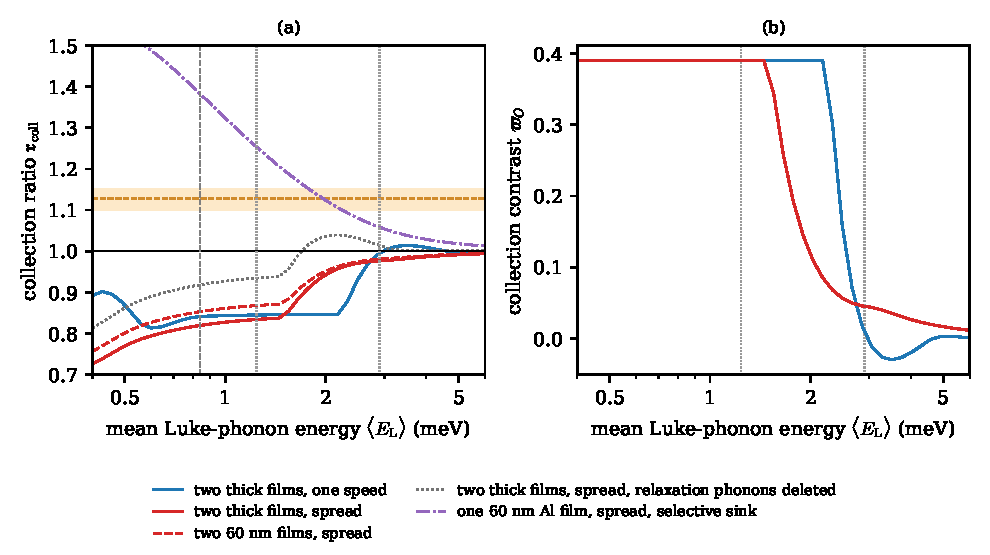
\includegraphics[width=\linewidth]{figures/ch20/fig20_rcoll.pdf}
  \caption{Mean-field collection of Luke phonons in a silicon slab \SI{4}{mm} thick, against the mean Luke-phonon energy. (a) Collection ratio $\mathfrak{r}_{\mathrm{coll}}$ of \cref{eq:20.5-functionals}. Solid: two thick films ($2\Delta_s = 3.0$ and \SI{0.36}{meV}, each on \SI{5}{\percent} of the face area) with the Kaplan-cascade yield of \cref{sec:20.4}, every phonon a film emits returned to the crystal, for the Luke spectrum of a carrier at one speed (blue, number density $\propto E_{\mathrm{ath}}^2$) and for a spread of speeds (red, flat number density up to $2\langle E_{\mathrm{L}}\rangle$). Red dashed: two \SI{60}{nm} films ($t_l/t_0 = 0.72$), spread, phonons returned. Gray dotted: two thick films, spread, with the phonons a film emits after its first pair break deleted. Purple dash-dotted: one \SI{60}{nm} aluminum film on \SI{10}{\percent} of the face area, spread, with the same deletion, a selective sink that the model does not identify in a detector (upper envelope). In all curves phonons below $2\Delta_{\mathrm{BCS}} = \SI{0.36}{meV}$ are reflected by the films and eventually lost. Tan band and dashed line: 1.099 to 1.152 and 1.128, the collection ratio that explains the silicon phonon-yield ratio of \cref{sec:19.5} with no stored energy. Vertical dashed line: \SI{0.84}{meV}, silicon electrons at \SI{1}{V/cm}; dotted: 1.24 and \SI{2.9}{meV}, the near-surface Luke energies of germanium~\cite{hertel2012phonon}. (b) Collection contrast $\varpi_O$ of the two thick films with phonons returned (channel 2 is the aluminum film), same colors. Model: transmission 0.9 into each film, bare-face loss $10^{-3}$ per hit, $\bar v = \SI{5.75}{km/s}$, $f_{\mathrm{LA}} = 0.093$, $A_{\mathrm{anh}} = \SI{7.41e-56}{s^4}$, $P_{\mathrm{d}}(y) = 60\,y^3(1 - y)^2$; primaries born at \SI{62}{meV}, absorbed in the two thick films with $\epsilon_{\mathrm{prim}} = 0.684$, $a_{\mathrm{prim}} = 0.610$.}
  \label{fig:20-rcoll}
\end{figure}

\Cref{fig:20-rcoll}(b) shows the contrast this geometry gives. While the whole Luke spectrum lies below the \SI{3}{meV} threshold of the niobium-like film, only aluminum absorbs Luke phonons, $a_{\mathrm{Luke}} = 1$, and $\varpi_O = 1 - a_{\mathrm{prim}} = 0.39$. As the mean energy rises, the Luke spectrum reaches above \SI{3}{meV} and the contrast falls: for the spread of speeds it is 0.12 at \SI{2}{meV}, 0.045 at \SI{2.9}{meV} and 0.019 at \SI{4.7}{meV}. In the mean-field limit the position spread vanishes by construction, so it is the first number a computed kernel adds.

\subsection{The sign of the collection ratio}\label{sec:20.5-sign}

The collection ratio differs from one through the part of the Luke spectrum within a few gaps of the aluminum threshold, since the primaries arrive at several meV. Luke energy below $2\Delta_{\mathrm{BCS}}$ of aluminum breaks no pairs; it is lost unless a tungsten sensor or another film absorbs it. Luke energy between $2\Delta_{\mathrm{BCS}}$ and $4\Delta_{\mathrm{BCS}}$ is converted with $Y_{\mathrm{qp}} = 2\Delta_{\mathrm{BCS}}/E_{\mathrm{ath}}$ in every film, above 0.59 below \SI{0.61}{meV} and down to 0.5 at $4\Delta_{\mathrm{BCS}}$ (\cref{sec:20.4}). Above four gaps a thick film converts with 0.59 to 0.60; a film from which phonons escape converts the primaries, at 14 to $44\,\Delta_{\mathrm{BCS}}$, with less than the soft Luke phonons on first absorption, but the phonons it lets out return to the crystal. And a phonon that only one film absorbs bounces longer before it is absorbed, and loses more on the bare faces.

The first two effects act alone in a detector with a single film type. Let $s_{\mathrm{sub}}$ be the share of Luke energy born below $2\Delta_{\mathrm{BCS}}$. Let sub-gap phonons be absorbed at the same rate as the others and converted with the weight $\kappa_{\mathrm{sub}}\bar Y_{\mathrm{prim}}$, where $\bar Y_{\mathrm{prim}}$ is the mean yield of the primaries as they are absorbed, and $\kappa_{\mathrm{sub}} = 0$ if they are lost and 1 if they are absorbed like hard phonons. Define the near-gap gain
\begin{equation*}
  s_{\mathrm{ng}} = \frac{1}{E_{\mathrm{Luke}}}\int_{2\Delta_{\mathrm{BCS}}}^\infty\dd E_{\mathrm{ath}}\;u_{\mathrm{Luke}}(E_{\mathrm{ath}})\Bigl[\frac{Y_{\mathrm{qp}}(E_{\mathrm{ath}})}{\bar Y_{\mathrm{prim}}} - 1\Bigr] .
\end{equation*}
If every phonon above the threshold reaches the film with the same probability per bounce, whatever its energy, the absorbed fraction is common to both populations and cancels in the ratio. The primaries are converted with $\bar Y_{\mathrm{prim}}$, the Luke phonons with $Y_{\mathrm{qp}}(E_{\mathrm{ath}})$ above the threshold and with $\kappa_{\mathrm{sub}}\bar Y_{\mathrm{prim}}$ below it, and
\begin{equation}
  \mathfrak{r}_{\mathrm{coll}} - 1 = s_{\mathrm{ng}} - (1 - \kappa_{\mathrm{sub}})\,s_{\mathrm{sub}} \qquad \text{(one film type)} .
  \label{eq:20.5-sign}
\end{equation}

The sub-gap share is fixed by the Luke spectrum alone. For the one-speed spectrum it is $s_{\mathrm{sub}} = 0.085$ at $\langle E_{\mathrm{L}}\rangle = \SI{0.5}{meV}$, 0.017 at \SI{0.75}{meV}, 0.011 at \SI{0.84}{meV} and $5\times10^{-3}$ at \SI{1}{meV}; for the spread of speeds 0.13, 0.058, 0.046 and 0.032, and still 0.008 at \SI{2}{meV}. In a thick film $\bar Y_{\mathrm{prim}} = 0.590$, and the near-gap gain is small: $+0.002$ for the one-speed spectrum and $+0.018$ for the spread of speeds at \SI{0.75}{meV}, since the cascade yield lies above 0.59 between 5 and $8\Delta_{\mathrm{BCS}}$ and below it near $4\Delta_{\mathrm{BCS}}$. With sub-gap phonons lost, one thick aluminum film then has $\mathfrak{r}_{\mathrm{coll}} = 0.985$ and 0.960 at \SI{0.75}{meV} and 0.994 and 0.968 at \SI{0.84}{meV}, below one by about $s_{\mathrm{sub}}$. If the sensor absorbs the sub-gap phonons, that term vanishes, and $\mathfrak{r}_{\mathrm{coll}} = 1.002$ to 1.018 between 0.75 and \SI{1}{meV}.

Escape does not change this when the phonons a film lets out return to the crystal. A returned phonon reaches a film again and continues the same cascade, so escape followed by return only delays it. For one aluminum film the solve gives the thick-film values within 0.002 at every $t_l/t_0$ down to the \SI{60}{nm} of \cref{we:20-escape}, 0.995 and 0.969 at \SI{0.84}{meV}. This is a numerical result, not an identity: bare-face loss and decay on the return path break it, and it holds at the bare-face loss of $10^{-3}$. A sink without signal that takes every phonon, modeled by raising the bare-face loss to 0.3 per hit, lowers $\epsilon_{\mathrm{prim}}$ to 0.08 and moves $\mathfrak{r}_{\mathrm{coll}}$ of the \SI{60}{nm} film only to 1.023 and 0.988. A large rise needs a selective sink, one that removes the phonons a film emits after its first pair break and leaves those that have not yet entered a film. The lumped film of \cref{sec:20.4} makes exactly that assumption. With it, the primaries are read at the yield of the band, about 0.50 at $t_l/t_0 = 4$ and 0.32 at 0.72, while the soft Luke energy keeps $2\Delta_{\mathrm{BCS}}/E_{\mathrm{ath}}$; the near-gap gain at \SI{0.75}{meV} becomes $+0.13$ and $+0.11$ at $t_l/t_0 = 4$ and $+0.61$ and $+0.49$ at 0.72, and one aluminum film at \SI{0.84}{meV} reaches 1.05 to 1.10 at $t_l/t_0 = 4$, about \SI{300}{nm}, and 1.30 to 1.53 at \SI{60}{nm}. These values are an upper envelope of the lumped-film assumption; the estimate does not identify a physical sink in a detector that would realize it.

The two-film geometry adds the third effect. Luke phonons below \SI{3}{meV} reach only the aluminum film, so they stay \SI{30}{\micro s} in the crystal against \SI{15}{\micro s} for phonons that both films absorb, and they lose twice as much on the bare faces, \SI{2.0}{\percent} against \SI{1.0}{\percent}. With a flat yield of 0.59 above each threshold and sub-gap phonons absorbed by the aluminum sensor, this alone gives $\mathfrak{r}_{\mathrm{coll}} = 0.992$, and with sub-gap phonons lost 0.935 at \SI{0.75}{meV} to 0.998 at \SI{4.7}{meV} for the spread of speeds. The film cascade with its returned phonons lowers these values further. The primaries reach the niobium-like film in large part, and its relaxation phonons, below \SI{3}{meV}, return and are collected by the aluminum film, which raises $\epsilon_{\mathrm{prim}}$ to 0.684; Luke phonons below \SI{3}{meV} gain nothing of the kind. Two thick films then give 0.83 and 0.81 at \SI{0.75}{meV} (one speed and spread), 0.84 and 0.82 at \SI{0.84}{meV}, and rise to 1.01 near \SI{3.5}{meV} for one speed, once the Luke spectrum itself reaches the niobium-like threshold. Two \SI{60}{nm} films give 0.85 to 1.01 over 0.75 to \SI{4.7}{meV}.

With every phonon a film emits returned to the crystal and energy conserved, the mean-field estimate lies between 0.81 and 1.02 over 0.75 to \SI{4.7}{meV}, one or two films, any film thickness from \SI{60}{nm} up, sub-gap phonons lost or absorbed, and between 0.82 and 1.01 at the \SI{0.84}{meV} of silicon electrons at \SI{1}{V/cm}. A signal-free sink acting on all phonons keeps it below 1.03. The collection ratio 1.128, with its band 1.099 to 1.152, that would explain the CDMS~II silicon phonon-yield ratio with no stored energy (\cref{sec:19.5}) therefore lies above the transport estimate; only the selective sink of the lumped film reaches it. Only computed kernels for real detector geometries can exclude collection as the whole explanation, and the two-bias measurement of \cref{sec:19.5} decides between collection and stored energy.

\subsection{Phonon signatures of the recoil type}\label{sec:20.5-routes}

A phonon readout separates the two recoils through an observable $O_{\mathrm{obs}}$ of each event, such as the channel fraction $E_2/(E_1 + E_2)$ or the share of the pulse in a fast window. At equal total phonon energy, the separation
\begin{equation}
  \mathcal{S}_{\mathrm{sep}} = \frac{\bigl|\langle O_{\mathrm{obs}}\rangle_{\mathrm{NR}} - \langle O_{\mathrm{obs}}\rangle_{\mathrm{ER}}\bigr|}{\bigl[\tfrac12\bigl(\sigma_{\mathrm{NR}}^2 + \sigma_{\mathrm{ER}}^2\bigr)\bigr]^{1/2}} ,
  \label{eq:20.5-sep}
\end{equation}
measures the distance between the two distributions in units of their spreads, and we call a route useful where $\mathcal{S}_{\mathrm{sep}} \ge 2$. For two Gaussians of equal width cut at the midpoint, $\mathcal{S}_{\mathrm{sep}} = 2$ accepts \SI{84}{\percent} of one population and rejects \SI{84}{\percent} of the other, and a leakage of $10^{-3}$ needs $\mathcal{S}_{\mathrm{sep}} = 6.2$, so ``useful'' is far from background-free. Let $\varphi_X$ be the share of population $X$ in the signal. Since the shares sum to one, the channel fraction is $O_{\mathrm{obs}} = \sum_Xa_X\varphi_X = a_{\mathrm{prim}} + \varpi_O\,\varphi_{\mathrm{Luke}} + \varpi_{\mathrm{gap}}\,\varphi_{\mathrm{gap}}$ after the average over positions, and another observable linear in the delivered energies has the same form to first order in the contrasts. There is one route for each population.

\paragraph{Primary phonons.} The prompt phonons forget their polarization within a nanosecond, and a hard birth once $E_*(t)$ has fallen to about half its energy (\cref{sec:20.2-memory}). The soft energy remains. It is the share $f_{\mathrm{s}} = \SI{1.7}{\percent}$ of an electron recoil that its carriers shed below the optical phonon energy, \cref{eq:20.2-fs}. A nuclear recoil has $Y_q$ times as many pairs, and its lattice share is born near the optical and zone-boundary energies (\cref{sec:19.1}). If $E_{\mathrm{mem}}$ lies above the soft band and below every hard birth, \cref{eq:20.2-bound} then gives
\begin{equation}
  \bigl|\langle O_{\mathrm{obs}}\rangle_{\mathrm{NR}} - \langle O_{\mathrm{obs}}\rangle_{\mathrm{ER}}\bigr| \simeq \varpi_{\mathrm{soft}}\,\Delta_{\mathrm{soft}} , \qquad \Delta_{\mathrm{soft}} = (1 - Y_q)\,f_{\mathrm{s}} ,
  \label{eq:20.5-primary}
\end{equation}
with $\varpi_{\mathrm{soft}}$ the contrast of the channel between soft primaries and hard ones. This is an estimate, not a bound (\cref{sec:20.2-bound}). At \SI{100}{eV}, $\Delta_{\mathrm{soft}} = 0.015$. The spread includes the position spread, so $\mathcal{S}_{\mathrm{sep}} \le \varpi_{\mathrm{soft}}\Delta_{\mathrm{soft}}/\sigma_{\mathrm{pos}}$, and any $\sigma_{\mathrm{pos}}$ above $\Delta_{\mathrm{soft}}/2 = 0.008$ excludes a useful separation at every energy, even with a perfect selector, $\varpi_{\mathrm{soft}} = 1$. The selector is far from perfect: the soft births have a few meV, and the mean-field estimate of \cref{sec:20.5-meanfield} puts the energy of the hard primaries at a mean of \SI{5.0}{meV} when they are absorbed, so no film threshold separates the two bands. The pulse shapes of CDMS detectors depend strongly on how close the event lies to each instrumented face~\cite[Sect.~2]{hertel2012phonon}, and a position correction must reach the percent level before this route opens. Phonons born within the memory-loss distance of an instrumented face keep some memory, but they mark a position class, not a recoil type (\cref{sec:20.2-memory}). None of this holds for sapphire, where isotope mixing is slower than decay and the memory argument of \cref{sec:20.2} fails.

\paragraph{Gap energy at zero field.} Each pair carries $\Eg$ until it recombines, so an electron recoil holds $\Eg/\varepsilon_{\mathrm{eh}} = 0.312$ of its energy in pairs, a nuclear recoil $Y_q$ times as much (\cref{sec:19.5}). If this energy comes back later than the primaries, a sensor with two read windows $t_1 < t_2$, with all gap energy returned by $t_2$, sees the ratio $O_b = E_{\mathrm{sig}}(t_1)/E_{\mathrm{sig}}(t_2)$. With $f_{\mathrm{ret}}(t)$ the returned fraction of \cref{eq:19.5-release}, no stored energy and equal collection,
\begin{equation}
  \Delta O_b = \frac{\Eg}{\varepsilon_{\mathrm{eh}}}\Bigl\{\bigl[1 - f^{\mathrm{ER}}_{\mathrm{ret}}(t_1)\bigr] - Y_q\bigl[1 - f^{\mathrm{NR}}_{\mathrm{ret}}(t_1)\bigr]\Bigr\} .
  \label{eq:20.5-gap}
\end{equation}
For equal release laws this is $(1 - Y_q)(\Eg/\varepsilon_{\mathrm{eh}})(1 - f_{\mathrm{ret}}) = 0.28\,(1 - f_{\mathrm{ret}})$ at \SI{100}{eV}, twenty times the primary estimate. The route is a timing reading of the pair number, and its size and sign are set by kinetics that are not known at millikelvin. In the dense track of a nuclear recoil, exciton annihilation gives $1 - f^{\mathrm{NR}}_{\mathrm{ret}} = 1/(1 + t/t_{\mathrm{rel}})$, with $t_{\mathrm{rel}}$ the time scale set by the initial track density (\cref{eq:19.5-bimol}). Against an exponential release $\ee^{-t/t_{\mathrm{rel}}}$ of the electron recoil on the same time scale, $\Delta O_b$ changes sign at the root of $\ee^{-x}(1 + x) = Y_q$, which is $t_1 = 3.87\,t_{\mathrm{rel}}$ at $Y_q = 0.102$. The site matters as much as the time. Release in the bulk produces hard phonons that lose their memory, and contributes nothing to $\varpi_{\mathrm{gap}}$. Release at a surface or an electrode produces soft phonons that travel ballistically, like the recombination phonons that carry \SI{13}{\percent} of the phonon signal of germanium detectors at \SI{3}{V} (\cref{sec:20.4-electrode}). The zero-field gap-energy channel is therefore unresolved.

\paragraph{Luke phonons at low bias.} With a bias the Luke share differs between the recoils because the pair number does. Let all pairs be drifted, with $g = f_{\mathrm{det}}\,g_{\mathrm{Luke}}$. An electron recoil then has $\varphi_{\mathrm{Luke}} = g/(1 + g)$ and a nuclear recoil $Y_qg/(1 + Y_qg)$. The gap shares differ in the same way, so
\begin{equation}
  \Delta O_{\mathrm{obs}} = \frac{(1 - Y_q)\,\bigl(\varpi_O\,g + \varpi_{\mathrm{gap}}\Eg/\varepsilon_{\mathrm{eh}}\bigr)}{(1 + g)(1 + Y_qg)} .
  \label{eq:20.5-lowbias}
\end{equation}
The Luke term is largest at $g = Y_q^{-1/2}$, where it equals $\varpi_O(1 - Y_q^{1/2})/(1 + Y_q^{1/2})$: at \SI{100}{eV}, $0.516\,\varpi_O$ at $g = 3.1$, or \SI{13.4}{V} across a silicon crystal at $f_{\mathrm{det}} = 0.873$. Whether the contrast suffices depends on the spreads. We compare the two recoils at the same recoil energy, \SI{100}{eV}, with the pair numbers of the measured yield in pairs of $\varepsilon_{\mathrm{eh}}$, $Y'_q$ of \cref{sec:20.5-hv}. The spread of $O_{\mathrm{obs}}$ for each recoil is the position spread, the baseline $\sigma_{\mathrm{ph}} = \SI{2.65}{eV}$ of the gram-scale detector~\cite{ren2021design} divided by that recoil's $E_{\mathrm{ph}}$, and the fluctuation of its detected pair number, $\varpi_O(eV_{\mathrm{bias}}/E_{\mathrm{ph}})(F_{\mathrm{meas}}N_{\mathrm{det}})^{1/2}$, added in quadrature. The binomial form of the measured-charge Fano factor, $F_{\mathrm{meas}} = f_{\mathrm{det}}F + 1 - f_{\mathrm{det}}$ (\cref{sec:20.1-fano}), uses the measured $F_{\mathrm{eh}} = 0.119$ for electron recoils, the measured $F_{\mathrm{NR}} = 0.9$ at \SI{100}{eV}~\cite[Table~II]{albakry2023first}, and $f_{\mathrm{det}} = 0.873$, the complement of the \SI{12.7}{\percent} trapping probability in the detector model of the same measurement. With $\varpi_{\mathrm{gap}} = 0$, the smallest contrast that reaches $\mathcal{S}_{\mathrm{sep}} = 2$ at \SI{100}{eV} is $\varpi_O = 0.11$, 0.22 and 0.43 for $\sigma_{\mathrm{pos}} = 0.02$, 0.05 and 0.10, at biases of 10 to \SI{12}{V}. The mean-field contrast of about 0.4 for Luke spectra below \SI{1.5}{meV} is within reach of this requirement, but it is a model, not a measurement. The route reads the pair number with phonons. Its ceiling, with $\varpi_O = 1$ and no other spread, is reached as the bias goes to zero, and it is that of the charge yield itself, 10.8 at \SI{100}{eV}: the route carries no information beyond the charge yield.

The phonon pulse-shape rejection of SuperCDMS germanium detectors is of this kind. It rejects bulk electron recoils against nuclear recoils at better than 1 in $10^3$ at 7 to \SI{20}{keV}, limited by the statistics of the data~\cite[Sect.~3]{hertel2012phonon}, and its information comes from Luke phonons emitted in the strong field near the surfaces.

\subsection{The high-voltage readout ceiling}\label{sec:20.5-hv}

At \SI{100}{V} across a silicon crystal, $g_{\mathrm{Luke}} = 26.7$ and the Luke phonons dominate the signal. Detectors run this way read the pair number through the total phonon energy, $E_{\mathrm{ph}} = E_{\mathrm{prim}} + N_{\mathrm{det}}eV_{\mathrm{bias}}$ with $N_{\mathrm{det}}$ the detected pairs (\cref{sec:1.5}), and an electron recoil of the same $E_{\mathrm{ph}}$ is the background to a nuclear recoil. Suppose a second observable reads the Luke share perfectly, with $\varpi_O = 1$, no baseline noise and no position spread. Its separation is the most any phonon observable can extract from the pair number at high bias.

A nuclear recoil of energy $E_R$ makes on average $Y_qE_R/\varepsilon_{\mathrm{src}}$ pairs, where $\varepsilon_{\mathrm{src}} = \SI{3.8}{eV}$ is the energy per pair with which the measurement converted its charge into the yields~\cite[Eq.~(1)]{albakry2023first}; write $Y'_q = Y_q\varepsilon_{\mathrm{eh}}/\varepsilon_{\mathrm{src}}$, so that the pair number is $Y'_qE_R/\varepsilon_{\mathrm{eh}}$. Its phonon energy is $E_{\mathrm{ph}} = E_R(1 + gY'_q)$, with $g = f_{\mathrm{det}}g_{\mathrm{Luke}}$ and the primary phonon energy taken equal to the recoil energy, the truncation of \cref{lim:19.5a} that the measurement uses. The electron recoil with the same $E_{\mathrm{ph}}$ has the energy $E_R(1 + gY'_q)/(1 + g)$. Their mean detected pair numbers are
\begin{equation*}
  \langle N_{\mathrm{det}}\rangle_{\mathrm{NR}} = f_{\mathrm{det}}Y'_q\frac{E_R}{\varepsilon_{\mathrm{eh}}} , \qquad
  \langle N_{\mathrm{det}}\rangle_{\mathrm{ER}} = f_{\mathrm{det}}\frac{E_R}{\varepsilon_{\mathrm{eh}}}\,\frac{1 + gY'_q}{1 + g} ,
\end{equation*}
and their difference is $f_{\mathrm{det}}(E_R/\varepsilon_{\mathrm{eh}})(1 - Y'_q)/(1 + g)$. The Luke share at fixed $E_{\mathrm{ph}}$ is linear in $N_{\mathrm{det}}$, so its separation is that of $N_{\mathrm{det}}$, with variances $F^X_{\mathrm{eff}}\langle N_{\mathrm{det}}\rangle_X$.
\begin{keyresult}[High-voltage readout ceiling]
With an ideal readout of the Luke share at equal total phonon energy, the separation of nuclear from electron recoils is
\begin{equation}
  \mathcal{S}_{\mathrm{HV}} = \frac{(1 - Y'_q)\,(f_{\mathrm{det}}E_R/\varepsilon_{\mathrm{eh}})^{1/2}}{\bigl\{\tfrac12(1 + g)\bigl[F^{\mathrm{NR}}_{\mathrm{eff}}\,Y'_q(1 + g) + F^{\mathrm{ER}}_{\mathrm{eff}}(1 + gY'_q)\bigr]\bigr\}^{1/2}} , \qquad g = f_{\mathrm{det}}\,g_{\mathrm{Luke}} ,
  \label{eq:20.5-hv}
\end{equation}
with $F_{\mathrm{eff}} = f_{\mathrm{det}}F + 1 - f_{\mathrm{det}}$ when a trapped carrier induces nothing and $F_{\mathrm{eff}} = f_{\mathrm{det}}F$ when every pair induces the mean charge $f_{\mathrm{det}}e$. The cascade and partial-charge terms of \cref{eq:20.1-Fpos} lie between these limits.
\end{keyresult}
\noindent At zero gain \cref{eq:20.5-hv} is the separation of an ideal charge-and-heat measurement. As the bias grows it falls as $1/g$, because at equal total phonon energy a larger Luke gain makes the electron recoil smaller, and the two pair numbers converge. In silicon at \SI{220}{eV} the ceiling is 16.8 at zero bias, 10.7 at \SI{4}{V}, 3.4 at \SI{30}{V}, 1.22 at \SI{100}{V} and 0.43 at \SI{300}{V}.

\begin{workedexample}{The high-voltage ceiling at 220 eV}\label{we:20-ceiling}
The measured silicon yield at $E_R = \SI{220}{eV}$ is $Y_q = 0.108^{+0.009}_{-0.010}$, with the pair-number Fano factor $F_{\mathrm{NR}} = 0.5^{+0.2}_{-0.1}$~\cite[Table~II]{albakry2023first}. At \SI{100}{V}, $g_{\mathrm{Luke}} = 100/3.75 = 26.67$, and with $f_{\mathrm{det}} = 0.873$, $g = 23.28$. The yield in pairs of \SI{3.75}{eV} is $Y'_q = 0.108\times3.75/3.8 = 0.1066$, and $E_R/\varepsilon_{\mathrm{eh}} = 58.67$.

The nuclear recoil has $E_{\mathrm{ph}} = 220\times(1 + 23.28\times0.1066) = \SI{765.9}{eV}$, and the electron recoil with the same phonon energy has $765.9/24.28 = \SI{31.54}{eV}$. The mean detected pair numbers are $0.873\times0.1066\times58.67 = 5.459$ and $0.873\times31.54/3.75 = 7.343$, a difference of 1.885 pairs.

With trapped carriers inducing nothing, $F^{\mathrm{NR}}_{\mathrm{eff}} = 0.873\times0.5 + 0.127 = 0.5635$ and $F^{\mathrm{ER}}_{\mathrm{eff}} = 0.873\times0.119 + 0.127 = 0.2309$. The variances are $0.5635\times5.459 = 3.076$ and $0.2309\times7.343 = 1.695$, and
\begin{equation*}
  \mathcal{S}_{\mathrm{HV}} = \frac{1.885}{[\tfrac12(3.076 + 1.695)]^{1/2}} = 1.22 .
\end{equation*}
If every pair induces the mean charge instead, the trapping term drops out of both Fano factors and $\mathcal{S}_{\mathrm{HV}} = 1.50$; with full collection, $f_{\mathrm{det}} = 1$, it is 1.32. Even an ideal phonon observable cannot separate the two recoils at \SI{220}{eV} and \SI{100}{V}.
\end{workedexample}

\begin{figure}[tbp]
  \centering
  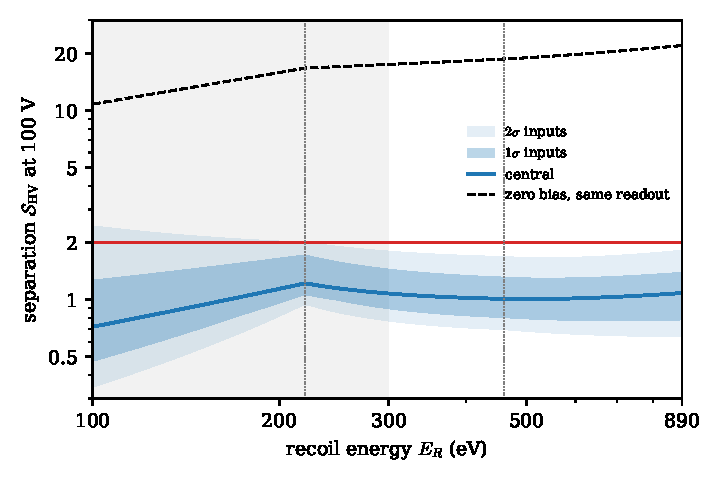
\includegraphics[width=0.8\linewidth]{figures/ch20/fig20_5.pdf}
  \caption{High-voltage readout ceiling $\mathcal{S}_{\mathrm{HV}}$ of \cref{eq:20.5-hv} for silicon recoils at \SI{100}{V}, against the recoil energy. Line: central measured yield and Fano factor~\cite[Table~II]{albakry2023first} at 100, 220, 460 and \SI{890}{eV} (dotted verticals), interpolated linearly in $\log E_R$; detected fraction $f_{\mathrm{det}} = 0.873$, trapped carriers inducing nothing; $F_{\mathrm{eh}} = 0.119$; $\varepsilon_{\mathrm{eh}} = \SI{3.75}{eV}$, yields defined with \SI{3.8}{eV} per pair. Dark band: the extremes over the corners of the $1\sigma$ bands of $Y_q$ and $F_{\mathrm{NR}}$, over $f_{\mathrm{det}} = 0.873$ and 1, and over the two limits of the induced-charge spread; light band: the same with $2\sigma$ bands. Dashed: the same ideal readout at zero bias. Red line: $\mathcal{S}_{\mathrm{HV}} = 2$. Gray: the range of the no-go statement, $E_R \le \SI{300}{eV}$.}
  \label{fig:20-ceiling}
\end{figure}

\Cref{fig:20-ceiling} extends the example over the measured range. At the central inputs the ceiling stays below 2 at every measured energy up to \SI{890}{eV}, with its maximum, 1.22, at \SI{220}{eV}; the Fano factor of nuclear recoils grows to 3.7 at \SI{890}{eV} and keeps it down. Over the $1\sigma$ bands of $Y_q$ and $F_{\mathrm{NR}}$ the largest value is 1.72, at \SI{220}{eV}, in the mean-charge limit. With $2\sigma$ bands the ceiling exceeds 2 from 100 to \SI{224}{eV}, up to 2.46 at \SI{100}{eV}, where the measured yield is least certain. The no-go of a high-voltage phonon readout at $E_R \le \SI{300}{eV}$ therefore rests on the measured $Y_q$ and $F_{\mathrm{NR}}$, which are not derived below the binary threshold of \cref{sec:19.2}, and on the collection, which moves the ceiling at \SI{220}{eV} between 1.22 and 1.50.

\subsection{Uncertainty budget of the readout}\label{sec:20.5-budget}

\Cref{tab:20-nuisances} is the uncertainty budget of the chapter.
\begin{table}[tbp]
  \caption{Uncertainty budget of charge, phonon and quasiparticle readout. Classes and bases as in \cref{tab:10-nuisances}; ``delayed'' moves charge or energy in time over an exposure.}
  \label{tab:20-nuisances}
  \centering\scriptsize\setlength{\tabcolsep}{3pt}
  \begin{tabular}{@{}>{\raggedright\arraybackslash}p{0.26\linewidth}>{\raggedright\arraybackslash}p{0.12\linewidth}>{\raggedright\arraybackslash}p{0.35\linewidth}>{\raggedright\arraybackslash}p{0.09\linewidth}>{\raggedright\arraybackslash}p{0.10\linewidth}@{}}
    \toprule
    Truncation or input & Type & Size & Basis & Section \\
    \midrule
    Exponential survival of drifting carriers & normali\-zation & collected fraction 0.632 (face), 0.736 (uniform) at $\lambda_{\mathrm{d}} = d_{\mathrm{det}}$; saturating drift velocity caps it below one & computed; model & \cref{sec:20.1} \\
    Fano factor of the measured charge & normali\-zation (width) & 0.125--0.158 at \SI{100}{eV}, \SI{95}{\percent} collection; position term $1.2\times10^{-4}\,\bar N_{\mathrm{eh}}$ & computed & \cref{sec:20.1} \\
    Space charge between flashes & delayed & \SI{1}{\percent} field change at \SI{1}{V/cm} for 6.3--$12.6\times10^4$ trapped charges per \si{cm^2} & est. & \cref{sec:20.1} \\
    Athermal emission from traps & delayed & cross-sections not computed & unsized & \cref{sec:20.1} \\
    Luke emission rate and spectrum & normali\-zation (of $\mathfrak{r}_{\mathrm{coll}}$, $\varpi_O$) & transverse emission omitted; mean energy \SI{0.84}{meV} for electrons at \SI{1}{V/cm} & model; unsized & \cref{sec:20.1,sec:20.5} \\
    Memory loss of prompt phonons & tilt & \SI{6.8}{ns} (Si), \SI{47}{ns} (Ge) near the band top; about \SI{1}{\micro s} for the \SI{22}{meV} daughters in Si; fails for sapphire & est. & \cref{sec:20.2} \\
    Interface transmission model & normali\-zation & $t_l$ differs by 1.31 between acoustic and diffuse mismatch; anisotropy: $\bar t_{\mathrm{esc}} = 0.327$--0.405 & model & \cref{sec:20.3} \\
    Quasiparticle yield above $4\Delta_{\mathrm{BCS}}$ & normali\-zation & 0.590 without escape; 0.349--0.554 at $10\Delta_{\mathrm{BCS}}$ for $t_l/t_0 = 0.5$--8; kinetic equations higher by up to 0.04 & model & \cref{sec:20.4} \\
    Soft primary share of an electron recoil & tilt & $f_{\mathrm{s}} \simeq 0.017$; $(1 - Y_q)f_{\mathrm{s}} = 0.015$ at \SI{100}{eV} & est. & \cref{sec:20.2,sec:20.5} \\
    Collection ratio of Luke phonons & normali\-zation & 0.81--1.02 (energy conserved); selective sink up to 1.53; 1.128 not reached; detector kernels not computed & model & \cref{sec:20.5} \\
    Collection contrast of Luke phonons & normali\-zation & 0.39 below about \SI{1.5}{meV}, 0.045 at \SI{2.9}{meV}; the low-bias route needs 0.11--0.43 & model & \cref{sec:20.5} \\
    Position spread of the channel fraction & normali\-zation & above 0.008 it closes the primary route & unsized & \cref{sec:20.5} \\
    Release law and site of the gap energy & tilt; delayed & two-window difference up to $0.28(1 - f_{\mathrm{ret}})$ at \SI{100}{eV}; sign not known & unsized & \cref{sec:20.5} \\
    Inputs of the high-voltage ceiling & threshold & \SI{220}{eV}, \SI{100}{V}: 1.22 (central), 1.50 (mean charge); 2.46 at \SI{100}{eV} with $2\sigma$ bands & input spread & \cref{sec:20.5} \\
    \bottomrule
  \end{tabular}
\end{table}

\section*{Summary}

A charge amplifier integrates the charge induced on its electrode (\cref{sec:20.1}). By Ramo's theorem each pair induces $e$ times the fraction of the gap its carriers cross, and the source does the work $eV_{\mathrm{bias}}$ times the same fraction, so trapping lowers the read charge and the Luke heat together. With exponential survival over a drift length $\lambda_{\mathrm{d}}$, the Hecht relation gives the collected fraction of a face event, and for $\lambda_{\mathrm{d}} \gg d_{\mathrm{det}}$ each carrier of a bulk event loses a third of what the carrier of a face event loses. The Fano factor of the measured charge has three terms, the cascade Fano factor scaled by the collection, the spread of partial charges and the spread of the mean collection over event positions; the last grows with the deposit. At \SI{95}{\percent} mean collection in silicon the measured Fano factor of a \SI{100}{eV} recoil lies between 0.125 and 0.158 depending on how the charge is lost. Trapped charge distorts the field over a finite part of the crystal by a percent at \SI{1}{V/cm} once some $10^5$ charges per \si{cm^2} are trapped, which ordinary event rates reach between flashes. Carriers faster than sound emit Luke phonons by the acoustic Cherenkov process. The mean phonon energy is \SI{0.84}{meV} for silicon electrons at \SI{1}{V/cm} in a transport Monte Carlo. The published total rates are low by a factor $k_{\mathrm{s}}/k$, and the emission from traps at millikelvin is not known.

The prompt phonons down-convert by anharmonic decay, at a rate $\propto E_{\mathrm{ath}}^5$ for longitudinal phonons, and scatter on isotopes at a rate $\propto E_{\mathrm{ath}}^4$ (\cref{sec:20.2}). Their spectrum approaches a scaling form in $E_{\mathrm{ath}}/E_*(t)$, and a hard birth is forgotten once $E_*$ has fallen to about half its energy. In bulk silicon this takes \SI{6.8}{ns} for births near the band top and about \SI{1}{\micro s} for the transverse daughters of optical decay. Near an instrumented face the birth is not forgotten, and at \SI{1}{\micro s} that region is \SI{13.5}{\percent} of a \SI{4}{mm} crystal. Polarization is forgotten within a nanosecond. These times are continuum estimates, and they do not hold for sapphire, where isotope mixing is slower than decay.

At the interface with a sensor film the averaged transmission is 0.938 from silicon into aluminum and 0.368 back, with the elastic constants of aluminum at zero temperature, tied by the reciprocity $\mathfrak{n}_1\bar t_{12} = \mathfrak{n}_2\bar t_{21}$ (\cref{sec:20.3}); \SI{56}{\percent} of the phonon flux in the film lies beyond the transverse critical angle and escapes only after mixing. A phonon leaves a film of thickness $d_{\mathrm{f}}$ in $t_l = 4d_{\mathrm{f}}/(v_s\bar t_{\mathrm{esc}})$, \SI{0.19}{ns} (acoustic mismatch) or \SI{0.24}{ns} (diffuse mismatch) for \SI{60}{nm} of aluminum, comparable to the pair-breaking time. The fitted silicon-to-aluminum coefficient of 0.3 to 0.55 is an absorption probability, and it constrains the ratio of pair-breaking length to film thickness to about 5 to 23 and leaves the escape probability unconstrained.

In the film a phonon between $2\Delta_{\mathrm{BCS}}$ and $4\Delta_{\mathrm{BCS}}$ breaks one pair and gives the quasiparticle yield $Y_{\mathrm{qp}} = 2\Delta_{\mathrm{BCS}}/E_{\mathrm{ath}}$ (\cref{sec:20.4}). Above $4\Delta_{\mathrm{BCS}}$ the Kaplan cascade gives 0.590 without escape, with a maximum of 0.600 at $5.46\,\Delta_{\mathrm{BCS}}$, and 0.349 to 0.554 at $10\Delta_{\mathrm{BCS}}$ for $t_l/t_0$ from 0.5 to 8; the yield then falls across the band in which down-converted phonons arrive. Carriers that reach an aluminum electrode return 85 to \SI{92}{\percent} of their energy at or below $2\Delta_{\mathrm{BCS}}$, phonons that cross the crystal ballistically.

The transport is linear in the birth spectrum, so a detector is described by the collection kernels of its sensors, and every readout quantity is a linear functional of them: the collection contrasts $\varpi_O$ and $\varpi_{\mathrm{gap}}$, the position spread and the collection ratio $\mathfrak{r}_{\mathrm{coll}}$ (\cref{sec:20.5}). In the mean-field limit, for a \SI{4}{mm} silicon slab with a niobium-like and an aluminum film, Luke phonons below \SI{3}{meV} reach only aluminum and $\varpi_O = 0.39$, falling to 0.045 at a mean Luke energy of \SI{2.9}{meV}. With one film type, $\mathfrak{r}_{\mathrm{coll}} - 1 = s_{\mathrm{ng}} - (1 - \kappa_{\mathrm{sub}})s_{\mathrm{sub}}$: the near-gap gain is small in thick films, and the share of Luke energy below $2\Delta_{\mathrm{BCS}}$ lowers the ratio if it is lost. Phonons that a film lets out return to the crystal and continue the same cascade, so film escape changes the ratio by less than 0.002. With energy conserved the estimate lies between 0.81 and 1.02 over mean Luke energies of 0.75 to \SI{4.7}{meV}. Only a selective sink that deletes the phonons a film emits after its first pair break, as the lumped film assumes, raises one aluminum film to between 1.05 and 1.53, an upper envelope. The value 1.128 that would explain the silicon phonon-yield ratio of \cref{sec:19.5} without stored energy therefore lies above the transport estimate; only computed kernels for real detectors can exclude it, and the two-bias measurement of \cref{sec:19.5} decides.

A phonon readout tells the recoil types apart only through their pair numbers. Mode, frequency or angle selection of the prompt phonons cannot separate nuclear from electron recoils in bulk silicon and germanium: only the soft share of an electron recoil, about \SI{1.5}{\percent} of its energy at \SI{100}{eV}, survives the memory loss, and a position spread of the channel fraction above 0.008 hides it. The zero-field gap-energy channel, up to $0.28$ of the recoil energy at \SI{100}{eV} in a two-window reading, is unresolved: its size and sign depend on the release law and site of the gap energy, which are not known at millikelvin. A low-bias readout of the Luke share reads the ionization yield with phonons and needs a contrast $\varpi_O$ of 0.11 to 0.43 for a position spread of 0.02 to 0.10 at \SI{100}{eV}. As the Luke gain grows, the pair numbers of the two recoils converge at equal total phonon energy, and at \SI{100}{V} even an ideal phonon observable separates silicon recoils of \SI{220}{eV} by only 1.22 standard deviations at the central measured yield and Fano factor. This no-go at $E_R \le \SI{300}{eV}$ holds over the $1\sigma$ bands of the measured inputs and fails at $2\sigma$. These verdicts are inputs to the readout column of the guide to next targets (\cref{sec:21.7}); all of them assume transport that has not yet been validated against the relations of this chapter.

\Cref{tab:20-nuisances} collects the truncations and inputs of the chapter with their sizes. The measured charge and phonon signals, with these conditions, are what the exclusion limits of the next chapter start from.

\begin{table}[tbp]
  \caption{Nuisances of charge, phonon and quasiparticle readout. Type in the classes of \cref{sec:8.8}, normalization, tilt, threshold and new support, with ``delayed'' for an item that moves charge or energy in time over an exposure. Basis of the size: ``computed'' (exact or next-order result computed), ``model'' (computed in a model), ``est.''\ (parametric estimate), ``input spread'' (spread or limitation of a measured or computed input), ``unsized'' (no size known). The last column gives the section where the item is treated.}
  \label{tab:20-nuisances}
  \centering\scriptsize\setlength{\tabcolsep}{3pt}
  \begin{tabular}{@{}>{\raggedright\arraybackslash}p{0.26\linewidth}>{\raggedright\arraybackslash}p{0.12\linewidth}>{\raggedright\arraybackslash}p{0.35\linewidth}>{\raggedright\arraybackslash}p{0.09\linewidth}>{\raggedright\arraybackslash}p{0.10\linewidth}@{}}
    \toprule
    Truncation or input & Type & Size & Basis & Section \\
    \midrule
    Exponential survival of drifting carriers & normali\-zation & collected fraction 0.632 (face), 0.736 (uniform) at $\lambda_{\mathrm{d}} = d_{\mathrm{det}}$; saturating drift velocity caps it below one & computed; model & \cref{sec:20.1} \\
    Fano factor of the measured charge & normali\-zation (width) & 0.125--0.158 at \SI{100}{eV}, \SI{95}{\percent} collection; position term $1.2\times10^{-4}\,\bar N_{\mathrm{eh}}$ & computed & \cref{sec:20.1} \\
    Space charge between flashes & delayed & \SI{1}{\percent} field change at \SI{1}{V/cm} for 6.3--$12.6\times10^4$ trapped charges per \si{cm^2} & est. & \cref{sec:20.1} \\
    Athermal emission from traps & delayed & cross-sections not computed & unsized & \cref{sec:20.1} \\
    Luke emission rate and spectrum & normali\-zation (of $\mathfrak{r}_{\mathrm{coll}}$, $\varpi_O$) & transverse emission omitted; mean energy \SI{0.84}{meV} for electrons at \SI{1}{V/cm} & model; unsized & \cref{sec:20.1,sec:20.5} \\
    Memory loss of prompt phonons & tilt & \SI{6.8}{ns} (Si), \SI{47}{ns} (Ge) near the band top; about \SI{1}{\micro s} for the \SI{22}{meV} daughters in Si; fails for sapphire & est. & \cref{sec:20.2} \\
    Interface transmission model & normali\-zation & $t_l$ differs by 1.31 between acoustic and diffuse mismatch; anisotropy: $\bar t_{\mathrm{esc}} = 0.327$--0.405 & model & \cref{sec:20.3} \\
    Quasiparticle yield above $4\Delta_{\mathrm{BCS}}$ & normali\-zation & 0.590 without escape; 0.349--0.554 at $10\Delta_{\mathrm{BCS}}$ for $t_l/t_0 = 0.5$--8; kinetic equations higher by up to 0.04 & model & \cref{sec:20.4} \\
    Soft primary share of an electron recoil & tilt & $f_{\mathrm{s}} \simeq 0.017$; $(1 - Y_q)f_{\mathrm{s}} = 0.015$ at \SI{100}{eV} & est. & \cref{sec:20.2,sec:20.5} \\
    Collection ratio of Luke phonons & normali\-zation & 0.81--1.02 (energy conserved); selective sink up to 1.53; 1.128 not reached; detector kernels not computed & model & \cref{sec:20.5} \\
    Collection contrast of Luke phonons & normali\-zation & 0.39 below about \SI{1.5}{meV}, 0.045 at \SI{2.9}{meV}; the low-bias route needs 0.11--0.43 & model & \cref{sec:20.5} \\
    Position spread of the channel fraction & normali\-zation & above 0.008 it closes the primary route & unsized & \cref{sec:20.5} \\
    Release law and site of the gap energy & tilt; delayed & two-window difference up to $0.28(1 - f_{\mathrm{ret}})$ at \SI{100}{eV}; sign not known & unsized & \cref{sec:20.5} \\
    Inputs of the high-voltage ceiling & threshold & \SI{220}{eV}, \SI{100}{V}: 1.22 (central), 1.50 (mean charge); 2.46 at \SI{100}{eV} with $2\sigma$ bands & input spread & \cref{sec:20.5} \\
    \bottomrule
  \end{tabular}
\end{table}

\printbibliography[heading=subbibliography]
